%%%%%%%%%%%%%%%%%%%%%%%%%%%%%%%%%%%%%%%%%%%%%%%%%%%%%%%%%%%%%%%
%% BRIEF VERSION OF OXFORD THESIS TEMPLATE FOR CHAPTER PREVIEWS

%%%%% CHOOSE PAGE LAYOUT
% format for PDF output (ie equal margins, no extra blank pages):
\documentclass[a4paper,nobind]{templates/ociamthesis}

% add hyperref package with links hidden %
\usepackage[colorlinks=false,pdfpagelabels,hidelinks]{hyperref}

% add float package to allow manual control of figure positioning %
\usepackage{float}

%UL set section header spacing
\usepackage{titlesec}
% 
\titlespacing\subsubsection{0pt}{24pt plus 4pt minus 2pt}{0pt plus 2pt minus 2pt}

% UL 30 Nov 2018 pandoc puts lists in 'tightlist' command when no space between bullet points in Rmd file
\providecommand{\tightlist}{%
  \setlength{\itemsep}{0pt}\setlength{\parskip}{0pt}}
 
% UL 1 Dec 2018, fix to include code in shaded environments
\usepackage{color}
\usepackage{fancyvrb}
\newcommand{\VerbBar}{|}
\newcommand{\VERB}{\Verb[commandchars=\\\{\}]}
\DefineVerbatimEnvironment{Highlighting}{Verbatim}{commandchars=\\\{\}}
% Add ',fontsize=\small' for more characters per line
\usepackage{framed}
\definecolor{shadecolor}{RGB}{248,248,248}
\newenvironment{Shaded}{\begin{snugshade}}{\end{snugshade}}
\newcommand{\AlertTok}[1]{\textcolor[rgb]{0.94,0.16,0.16}{#1}}
\newcommand{\AnnotationTok}[1]{\textcolor[rgb]{0.56,0.35,0.01}{\textbf{\textit{#1}}}}
\newcommand{\AttributeTok}[1]{\textcolor[rgb]{0.77,0.63,0.00}{#1}}
\newcommand{\BaseNTok}[1]{\textcolor[rgb]{0.00,0.00,0.81}{#1}}
\newcommand{\BuiltInTok}[1]{#1}
\newcommand{\CharTok}[1]{\textcolor[rgb]{0.31,0.60,0.02}{#1}}
\newcommand{\CommentTok}[1]{\textcolor[rgb]{0.56,0.35,0.01}{\textit{#1}}}
\newcommand{\CommentVarTok}[1]{\textcolor[rgb]{0.56,0.35,0.01}{\textbf{\textit{#1}}}}
\newcommand{\ConstantTok}[1]{\textcolor[rgb]{0.00,0.00,0.00}{#1}}
\newcommand{\ControlFlowTok}[1]{\textcolor[rgb]{0.13,0.29,0.53}{\textbf{#1}}}
\newcommand{\DataTypeTok}[1]{\textcolor[rgb]{0.13,0.29,0.53}{#1}}
\newcommand{\DecValTok}[1]{\textcolor[rgb]{0.00,0.00,0.81}{#1}}
\newcommand{\DocumentationTok}[1]{\textcolor[rgb]{0.56,0.35,0.01}{\textbf{\textit{#1}}}}
\newcommand{\ErrorTok}[1]{\textcolor[rgb]{0.64,0.00,0.00}{\textbf{#1}}}
\newcommand{\ExtensionTok}[1]{#1}
\newcommand{\FloatTok}[1]{\textcolor[rgb]{0.00,0.00,0.81}{#1}}
\newcommand{\FunctionTok}[1]{\textcolor[rgb]{0.00,0.00,0.00}{#1}}
\newcommand{\ImportTok}[1]{#1}
\newcommand{\InformationTok}[1]{\textcolor[rgb]{0.56,0.35,0.01}{\textbf{\textit{#1}}}}
\newcommand{\KeywordTok}[1]{\textcolor[rgb]{0.13,0.29,0.53}{\textbf{#1}}}
\newcommand{\NormalTok}[1]{#1}
\newcommand{\OperatorTok}[1]{\textcolor[rgb]{0.81,0.36,0.00}{\textbf{#1}}}
\newcommand{\OtherTok}[1]{\textcolor[rgb]{0.56,0.35,0.01}{#1}}
\newcommand{\PreprocessorTok}[1]{\textcolor[rgb]{0.56,0.35,0.01}{\textit{#1}}}
\newcommand{\RegionMarkerTok}[1]{#1}
\newcommand{\SpecialCharTok}[1]{\textcolor[rgb]{0.00,0.00,0.00}{#1}}
\newcommand{\SpecialStringTok}[1]{\textcolor[rgb]{0.31,0.60,0.02}{#1}}
\newcommand{\StringTok}[1]{\textcolor[rgb]{0.31,0.60,0.02}{#1}}
\newcommand{\VariableTok}[1]{\textcolor[rgb]{0.00,0.00,0.00}{#1}}
\newcommand{\VerbatimStringTok}[1]{\textcolor[rgb]{0.31,0.60,0.02}{#1}}
\newcommand{\WarningTok}[1]{\textcolor[rgb]{0.56,0.35,0.01}{\textbf{\textit{#1}}}}

%UL 2 Dec 2018 add a bit of white space before and after code blocks
\renewenvironment{Shaded}
{
  \vspace{10pt}%
  \begin{snugshade}%
}{%
  \end{snugshade}%
  \vspace{8pt}%
}
%UL 2 Dec 2018 reduce whitespace around verbatim environments
\usepackage{etoolbox}
\makeatletter
\preto{\@verbatim}{\topsep=0pt \partopsep=0pt }
\makeatother

%UL 28 Mar 2019, enable strikethrough
\usepackage[normalem]{ulem}

%UL use soul package for correction highlighting
\usepackage{soul}
\usepackage{xcolor}
\newcommand{\ctext}[3][RGB]{%
  \begingroup
  \definecolor{hlcolor}{#1}{#2}\sethlcolor{hlcolor}%
  \hl{#3}%
  \endgroup
}
\soulregister\ref7
\soulregister\cite7
\soulregister\autocite7
\soulregister\textcite7
\soulregister\pageref7

% user-included things with header_includes or in_header will appear here
% kableExtra packages will appear here if you use library(kableExtra)

%%%%% SELECT YOUR DRAFT OPTIONS
% Three options going on here; use in any combination.  But remember to turn the first two off before
% generating a PDF to send to the printer!

% This adds a "DRAFT" footer to every normal page.  (The first page of each chapter is not a "normal" page.)

% This highlights (in blue) corrections marked with (for words) \mccorrect{blah} or (for whole
% paragraphs) \begin{mccorrection} . . . \end{mccorrection}.  This can be useful for sending a PDF of
% your corrected thesis to your examiners for review.  Turn it off, and the blue disappears.

%%%%% BIBLIOGRAPHY SETUP
% Note that your bibliography will require some tweaking depending on your department, preferred format, etc.
% The options included below are just very basic "sciencey" and "humanitiesey" options to get started.
% If you've not used LaTeX before, I recommend reading a little about biblatex/biber and getting started with it.
% If you're already a LaTeX pro and are used to natbib or something, modify as necessary.
% Either way, you'll have to choose and configure an appropriate bibliography format...

% The science-type option: numerical in-text citation with references in order of appearance.
% \usepackage[style=numeric-comp, sorting=none, backend=biber, doi=false, isbn=false]{biblatex}
% \newcommand*{\bibtitle}{References}

% The humanities-type option: author-year in-text citation with an alphabetical works cited.
% \usepackage[style=authoryear, sorting=nyt, backend=biber, maxcitenames=2, useprefix, doi=false, isbn=false]{biblatex}
% \newcommand*{\bibtitle}{Works Cited}

%UL 3 Dec 2018: set this from YAML in index.Rmd
\usepackage[style=numeric-comp, sorting=none, backend=biber, doi=false, isbn=false]{biblatex}
\newcommand*{\bibtitle}{References}

% This makes the bibliography left-aligned (not 'justified') and slightly smaller font.
\renewcommand*{\bibfont}{\raggedright\small}

% Change this to the name of your .bib file (usually exported from a citation manager like Zotero or EndNote).

%%%%% YOUR OWN PERSONAL MACROS
% This is a good place to dump your own LaTeX macros as they come up.

% To make text superscripts shortcuts
	\renewcommand{\th}{\textsuperscript{th}} % ex: I won 4\th place
	\newcommand{\nd}{\textsuperscript{nd}}
	\renewcommand{\st}{\textsuperscript{st}}
	\newcommand{\rd}{\textsuperscript{rd}}

%%%%% THE ACTUAL DOCUMENT STARTS HERE
\begin{document}

%%%%% CHOOSE YOUR LINE SPACING HERE
% This is the official option.  Use it for your submission copy and library copy:
\setlength{\textbaselineskip}{22pt plus2pt}
% This is closer spacing (about 1.5-spaced) that you might prefer for your personal copies:
%\setlength{\textbaselineskip}{18pt plus2pt minus1pt}

% UL: You can set the general paragraph spacing here - I've set it to 2pt (was 0) so
% it's less claustrophobic
\setlength{\parskip}{2pt plus 1pt}

% Leave this line alone; it gets things started for the real document.
\setlength{\baselineskip}{\textbaselineskip}

% all your chapters and appendices will appear here
\hypertarget{chapter-1-insert-title}{%
\chapter{Chapter 1: INSERT TITLE}\label{chapter-1-insert-title}}

\hypertarget{introduction}{%
\section{Introduction}\label{introduction}}

\hypertarget{gender-gaps-persist-despite-womens-success-in-education---researchers-are-focusing-on-psychological-differences-such-as-competition-preferences-as-explanation}{%
\section{Gender gaps persist despite women's success in education - researchers are focusing on psychological differences, such as competition preferences, as explanation}\label{gender-gaps-persist-despite-womens-success-in-education---researchers-are-focusing-on-psychological-differences-such-as-competition-preferences-as-explanation}}

Women have surpassed men in education outcomes, like college attendance and graduation rates \autocite{Blau2017,Goldin2006,Stoet2014}, but continue to be underrepresented in top management positions in nearly all sectors \autocite{Bertrand2001}. And, a sizable gender gap still persists worldwide \autocite{Blau2017}. Traditional economic variables, such as household division of labor and discrimination, account for some, but not all, of these disparities \autocite{Blau2017}. As such, researchers have begun to consider psychological gender differences, including the predilection for competition, as means of understanding persistent gender gaps in labor market outcomes \autocite[for review, see][]{Niederle2011}.

\hypertarget{overview-of-lit-on-choice-to-compete---niederle2007-replications-task-type-effects}{%
\section{Overview of lit on choice to compete - niederle2007, replications, task type effects}\label{overview-of-lit-on-choice-to-compete---niederle2007-replications-task-type-effects}}

Research suggests women are, on average, less competitive than men (for review, see \textcite{Niederle2011}). Foundational work on gender differences in competitiveness operationalized competitiveness as the choice of a tournament payment scheme, that reaps potentially higher earnings but requires outperforming an opponent, over a piece-rate scheme, where participants are paid per unit of work they produce \autocite{Niederle2007}. In this paradigm, women are less likely to enter tournaments while completing mathematical problems, even when they would have earned more by competing \autocite{Niederle2007}. Numerous conceptual replications over the past 15 years suggest that the gender difference in willingness to compete is robust \autocites[see][ for review]{Niederle2011,Niederle2017a,Niederle2017b}. Notably, this effect has been replicated in diverse populations (e.g., across age groups and cultures) \autocite{Apicella2015,Buser2014,Sutter2016,Andersen2013,Buser2017b,Sutter2010,Dreber2014,Mayr2012} and with a diverse set of tasks \autocite{Apicella2015,Saccardo2018,Bjorvatn2016,Sutter2015,Frick2011,Samek2019}. However, there is evidence that the task used during competition affects the size of the gender gap. For instance, some research suggests that when the task is female-typed or gender-neutral, the gender gap in willingness to compete may be reduced or eliminated \autocite{Iriberri2017,Boschini2014,Boschini2019,Apicella2015,Grosse2010,Gunther2010,Dreber2014,Dreber2011,Shurchkov2012}. Drawing from the psychology literature on stereotype threat \autocite{Steele1997,Spencer1999,Spencer2016}, negative stereotypes about women's ability to perform male-typed tasks (e.g., math, mental rotation) may produce anxiety and undermine performance. As a result, women may decide not to engage in a competition because they either believe the stereotype or because the stereotype provokes enough anxiety to reduce performance \autocite{Gunther2010,Grosse2010,Iriberri2017,Shurchkov2012}.

\hypertarget{choice-to-compete-as-measured-in-lit-predicts-real-world-outcomes-so-interventions-may-reduce-gender-gaps}{%
\section{Choice to compete as measured in lit predicts real world outcomes, so interventions may reduce gender gaps}\label{choice-to-compete-as-measured-in-lit-predicts-real-world-outcomes-so-interventions-may-reduce-gender-gaps}}

Importantly, this laboratory measure of competitiveness predicts labor market outcomes, including education choices \autocite{Buser2014,Zhang2012}, entrepreneurial decisions {[}e.g., investment, employment; \textcite{Berge2015}{]}, and earnings \autocite{Reuben2015}. In other words, competitive preferences may contribute to the gender gap in labor market outcomes \autocite{Blau2017}. Thus, understanding why men and women differ in levels of competitiveness and whether interventions exist that can reduce or eliminate the difference may be key for solving the pernicious gender gaps in the labor market.

\hypertarget{risk-attitude-and-confidence-as-proposed-mechanisms-for-gender-difference-in-competitiveness}{%
\section{Risk attitude and confidence as proposed mechanisms for gender difference in competitiveness}\label{risk-attitude-and-confidence-as-proposed-mechanisms-for-gender-difference-in-competitiveness}}

Both confidence and risk attitudes have been implicated in driving gender differences in willingness to compete \autocite{Niederle2011,Veldhuizen2017}. However, the extent to which confidence and risk attitudes account for the gender difference in willingness to compete is debated. The foundational research in this literature suggests that confidence and risk attitudes do not completely explain gender differences in competitiveness, since there remained a residual gap after controlling for these factors \autocite{Niederle2007}. As a result, the unexplained component of the original gender effect was taken as evidence of a distinct ``competitiveness'' trait, separate from risk attitudes and confidence \autocite{Niederle2007,Niederle2011}. Conversely, recent work correcting for measurement error \autocite{Gillen2019} and using experimental techniques to isolate the effects of the competitiveness trait \autocite{Veldhuizen2017} suggests that risk attitudes and confidence can fully explain the gender gap in the choice to compete.

Regardless of whether competitiveness is a ``stand-alone'' trait, it is clear that both confidence and risk attitudes influence how men and women react to competitions. For instance, even in the original study by Niederle and Vesterlund (2007), 27\% of the gender gap in tournament entry was explained by men being more overconfident than women about their relative performance on the task. As such, interventions designed to correct men's overconfidence, increase women's confidence, or decrease women's perceptions of risk and uncertainty in competitive contexts may help reduce the gender gap in competitiveness.

\hypertarget{gender-differences-in-confidence}{%
\subsection{Gender differences in confidence}\label{gender-differences-in-confidence}}

Within the literature on the gender gap in competitiveness, confidence is operationalized as the belief about one's relative performance during a competition, where individuals who have inaccurately high (low) ratings of their performance are deemed overconfident (underconfident) \autocites{Niederle2011}[also see overplacement in][]{Moore2008}. If an individual does not believe their performance is higher than the individuals they are competing against, they are unlikely to make the decision to compete for fear of losing.

While most individuals are overconfident \autocite{Alicke2013,Dunning2004b}, there is ample research to suggest that women are less (over)confident on average than men across a number of domains \autocite{Mobius2011,Niederle2011,Croson2009,Lundeberg1994,Niederle2007,Bertrand2010a,Beyer1990,Beyer1997,Jakobsson2013}. Because women are less overconfident, they compete less often than they should, given their actual ability \autocite{Niederle2007}. Confidence too may help explain why, in some situations, the gender gap in competitiveness may be reduced or eliminated. For instance, women tend to compete more when tasks are female-typed or gender-neutral \autocite{Iriberri2017,Boschini2014,Boschini2019,Apicella2015,Grosse2010,Gunther2010,Dreber2014,Dreber2011,Shurchkov2012}, when they are facing other women \autocite{DattaGupta2013,Booth2012}, or when competing against themselves \autocite{Apicella2017a,Bonte2018,Carpenter2018,Apicella2020}. For example, Apicella et al.~(2017) document a gender difference in confidence when women and men are competing against other individuals, but not when they are competing against themselves (i.e., their own past performance). There are several non-mutually exclusive and potentially interacting explanations that could account for women's relatively lower (over)confidence, including differences in performance or ability, experience, innate psychological differences, and stereotype threat \autocite{Steele1997,Spencer1999,Spencer2016}. In the latter case, for instance, women may decide to forgo competitions because they either believe negative stereotypes about their ability to perform certain tasks, or because stereotypes provoke enough anxiety to reduce confidence \autocite{Gunther2010,Grosse2010,Iriberri2017,Shurchkov2012,Burow2017}. Taken together, this body of research suggests that interventions designed to increase confidence in women, may embolden them to compete more.

\hypertarget{gender-differences-in-risk-attitude}{%
\subsection{Gender differences in risk attitude}\label{gender-differences-in-risk-attitude}}

A second variable that has been identified as a possible explanation for gender differences in competitiveness is risk attitudes, typically construed as the preference for a certain gain over a gamble, even if the gamble has an equal or greater monetary expectation \autocite{Kahneman1982}. Researchers investigating gender differences in risk attitudes find that men are typically more risk-seeking than women \autocite{Eckel2008,Charness2012,Croson2009,Bertrand2010a}, including in hunter-gatherers \autocite{Apicella2017}, but see \autocite{Harrison2007} for an exception. While most studies report a gender difference, the difference appears to be small to medium \autocite{Filippin2016} and culturally-dependent {[}Anderson, et al.~2013; \textcite{Gneezy2009}{]}.

Competitive payment schemes are inherently riskier than piece-rate payment schemes because the variance in returns is greater. With piece-rate payment schemes, individuals are guaranteed a certain amount for every unit they produce. Moreover, there typically exists uncertainty in competitions since one's relative performance is unknown \autocite{Niederle2011}. Indeed, some of the gender gap in competitiveness is explained by men and women's differing risk attitudes \autocite{Niederle2011}. In fact, some recent work suggests that nearly 30\% of the gender gap in competitive choices can be explained by risk attitudes \autocite{Gillen2019,Veldhuizen2017}.

\hypertarget{why-preparation-may-eliminate-gender-gap-in-competitiveness-by-changing-confidence-andor-risk-attitude}{%
\section{Why preparation may eliminate gender gap in competitiveness by changing confidence and/or risk attitude}\label{why-preparation-may-eliminate-gender-gap-in-competitiveness-by-changing-confidence-andor-risk-attitude}}

Preparation or training on a task may increase one's confidence \autocite{Gist1992,Schunk1981,Schunk1982,Usher2008}, since people usually are able to observe an improvement in their performance over time. \textcite{Lent1996} found that college students listed past accomplishments as the most influential factor in determining their confidence. Moreover, research directly comparing the effects of mastery experiences (via preparation), vicarious experiences (e.g., watching others perform a task), and a control treatment without any intervention on confidence, found that mastery increased confidence significantly more than vicarious experiences and the control treatment \autocite{Bandura1977a}. Other research suggests that men and women's confidence is similar in domains in which they have expertise, but the confidence gap emerges when it is assessed in less knowledgeable domains \autocite{Sarsons2016}. This suggests that gaining expertise, perhaps through practicing, may selectively boost women's confidence. \textcite{Roll2011} found that practicing mathematics problems, using an intelligent tutoring system, significantly decreases underconfidence but has no effect on rates of overconfidence. This too suggests that practicing may preferentially benefit women who are more likely than men to be underconfident. That said, if practicing only helps with underconfidence, when most people, including women, are overconfident, then its application may be limited.

Preparation, and the feelings of preparedness or self-efficacy that follow, may also decrease the perceived riskiness of competitions. With increased self-efficacy, individuals may believe they can reduce risk or overcome adversity. Surprisingly little work has explored how preparation impacts men's and women's risk attitudes. However, some experimental work suggests that manipulating perceived competence on a task by giving participants positive feedback about their performance on a task can lead to significantly more risk-taking behavior \autocite{Krueger1994}. The researchers were able to rule out the role of mood in driving the results by giving some participants positive feedback on one task and negative feedback on another. For these participants, risk-taking increased in the positive feedback condition and decreased in the negative feedback condition. Interestingly, \textcite{Gysler2002} find that knowledge -- in this case, understanding of financial markets -- and confidence in that knowledge, negatively correlate with women's risk aversion, but positively correlate with men's risk aversion. This suggests that preparation may disproportionately increase risk-taking in women. Finally, there is evidence that risk attitudes play a greater role in predicting decisions to compete when individuals are competing against other individuals, rather than themselves (i.e., their own past performance), possibly because there is more uncertainty in estimating an opponent's ability versus one's own ability \autocite{Apicella2017a}.

\hypertarget{previous-literature-looking-at-preparation-on-competition-entry}{%
\section{Previous literature looking at preparation on competition entry}\label{previous-literature-looking-at-preparation-on-competition-entry}}

Surprisingly, little work has explored how preparation impacts men and women's confidence, risk attitudes, or their willingness to compete. We know of only one study that has explored how delaying a competition, and in some cases, offering an opportunity to study, affects decisions to compete. In a working paper, \textcite{Charness2021} examine whether gender gap entry rates change when a future opportunity to study for the task is made available. The authors hypothesized that women would be more likely to compete when there is an opportunity to study for the task. Contrary to their prediction, the authors found that providing an option to study leads men to be more likely to enter into future planned tournaments and leads women to be less likely to enter into these tournaments, resulting in a significant gender gap. However, this gap was only present during the initial, provisional sign-up period. When the actual choice was made later -- sometime between one and five days -- the gender difference disappeared. Of those men who returned to complete the study, some switched into the non-competitive payment scheme. The authors suggest that the results may be explained by men being overly confident in their future selves' resolve to study.

\hypertarget{the-current-experiments}{%
\section{The current experiments}\label{the-current-experiments}}

We examine the role of preparation on the gender differences in willingness to compete through three experiments. However, unlike \textcite{Charness2021}, we do not introduce a significant time delay in our studies. That is, experiments took place in a single session, thus minimizing any potential for gender differences in beliefs about future behavior to affect our results.

In the first experiment, we test whether simply knowing that there will be an opportunity to prepare before performing a task affects the gender gap in willingness to compete. That is, we manipulate participants' knowledge of whether they will have time to prepare before they make their decision to compete. We anticipated that participants with this information would be more inclined to compete compared to participants without this information and that this effect would be stronger for women, who tend to be relatively less confident. Thus, we expected a main effect of condition and an interaction between gender and condition on the choice to compete. In the second experiment, we examined how actual preparation influences the decision to compete. That is, we manipulated whether participants were required to prepare before making the decision to compete. Again, we expected that women in the preparation condition would be more inclined to compete than women in the no preparation condition, while we did not expect men's competitiveness to be significantly affected by the preparation manipulation.

Finally, in experiment 3, we examine how an unlimited amount of preparation affects gender differences in the willingness to compete. Across all experiments, we measured gender differences in actual preparation after administering the treatment and eliciting preferences to compete. Finally, we monetarily incentivized participants in both studies to correctly predict whether men or women would prepare and compete more. The research design, hypotheses, measures and analyses were pre-registered on \href{https://osf.io/q39a5/}{OSF} and all analyses were conducted in R statistical software (version 4.0.4). All participants across the three experiments were recruited through Amazon Mechanical Turk (or MTurk), with a guaranteed payment and the opportunity to earn bonuses depending on their performance and the performance of others. Recruiting participants on this platform allowed for efficient data collection while meeting acceptable psychometric standards, such as high test-retest and alpha reliability \autocite{Rand2012,Buhrmester2011}.

\hypertarget{study-1}{%
\section{Study 1}\label{study-1}}

\hypertarget{methods}{%
\subsection{Methods}\label{methods}}

INSERT: Participants' scores on the task will be quantified as the number of questions correct within the two-minute time frame allotted, without any penalties for incorrect responses. Afterwards, participants will be informed of the number of questions they answered correctly. We do not include any information about their relative performance since we ask them to guess their relative performance in the confidence measure. Thus, participants following the tournament payment scheme will not be told whether they won, since this serves as an indicator of relative performance. We employ this strategy across all studies in this dissertation.

POSSIBLY INSERT:
After completing the task, participants will complete a series of measures to be used for exploratory analyses. All questions will be counterbalanced. A confidence measure will incentivize participants to guess their relative performance compared to all other participants that completed the task by indicating the decile of their score relative to other participants. If correct, participants will earn \$.25. We use a measure of relative performance, rather than a measure of absolute performance (e.g., asking participants to guess their score on the task) because perceptions of relative performance will likely be predictive of the choice to practice, especially when an individual is required to compete. The confidence measure draws from previous research \autocite{Niederle2007}, but instead of asking participants to indicate whether they won against a randomly selected opponent, we ask them to guess their relative decile to provide us with more information about their relative confidence. Given the difficulty of guessing one's exact percentile without any information about other participants, deciles are used rather than percentiles to make earning the bonus seem more achievable. Also, the item will be phrased so participants do not need to understand the word ``decile,'' but will be asked ``If my performance is compared to that of all participants that completed the task, I think my score was\ldots{}'' with the options for responses ranging from ``Better than all other participants'' to ``Better than none of the other participants'' with 10\% increments in between (e.g., ``Better than 50\% of participants''). Since task-specific confidence measures tend to be better predictors of behavior than general measures of confidence \autocite[see][ for review]{Oney2015}, the confidence measure assesses participants' beliefs within the context of the task used. We will also measure risk attitude by asking participants to indicate on a 0-10 scale ``How do you see yourself: Are you generally a person who is fully prepared to take risks or do you try to avoid taking risks?'' \autocite{Dohmen2011b}. There is evidence that risky behavior (i.e., lottery choices) is strongly associated with the risk measure included in the current proposal \autocite{Dohmen2011b}. Additionally, risk attitude tends to be explained by one underlying trait, with a relatively smaller amount of variation in risk attitude explained by context (e.g., risk attitude during career, health, or financial decisions). Thus, across contexts, risk attitude is likely to be stable and predictive of behavior \autocite{Dohmen2011b}. These measures are included after completing the task largely because the confidence measure requires participants to state their perceived relative performance on the task.

Participants on Amazon Mechanical Turk who opted into the study had to pass several screening questions. Specifically, participants included in the paid portion of the study had to (i) identify their nationality as American and live in the United States, (ii) identify as a man or a woman, and (iii) be using a computer (rather than a phone or tablet). If they did not meet these criteria, they did not proceed to the paid portion of the study. Additionally, upon reviewing the data, we had reason to suspect that some participants completed the study more than once. Specifically, some participants had the same IP address, MTurk ID, and were of the same gender. When entries matched on all three identifiers, we included only the first entry and excluded all subsequent entries. The final sample consisted of 1056 participants (53.6\% women), with an average age of 37.74 (\emph{SD} = 13.19) years. 54 participants (53.7\% women) dropped out of the study before finishing and we use their data when available.

Participants were told they would be completing a timed multiplication task where they could choose how they would be paid for their performance. We chose a multiplication task because we expected participants' performance to improve with practice. Indeed, research suggests that rehearsing and recalling associative memories can speed up retrieval of those memories \autocite{Rundus1971}. The task involved solving problems from multiplication tables 1-12 as quickly as possible within a two-minute period. They were provided an example of a question with the correct response and had to answer three practice problems correctly to proceed, as a test of their comprehension. After completing the comprehension questions, participants were randomly assigned to either a ``knowledge of preparation'' condition or a control condition. Participants in the ``knowledge of preparation'' condition were presented the following text:

``There is an option to practice/study before completing the multiplication task that is available to all participants. If you take this opportunity to practice/study, we will provide you with materials that may help boost your performance in the multiplication task. You will have unlimited time to practice/study before completing the task. You can stop practicing/studying at any point.''

Participants assigned to the control condition simply proceeded without seeing this text. An equal number of participants were assigned to both conditions (control= 50\%). Of the men who completed the study, 49.59\% were randomly assigned to the control condition. Of the women who completed the study, 49.29\% were randomly assigned to the control condition, \(\chi^2(1, n = 1056) = 0.00\), \(p > .999\).

Then, all participants were asked to choose how they wanted to be paid. They were given two options, either a piece-rate payment scheme or a tournament payment scheme. They first read a description of each payment scheme, and had to correctly answer three comprehension questions before making their selection.

Under the piece-rate scheme participants were told that they would be paid \$.10 for every problem answered correctly. Under the tournament scheme, participants were told that they would be paid \$.20 for every problem they answered correctly, but only if they answered more questions correctly than a randomly assigned competitor. The order of presentation of the tournament and piece-rate payment options was randomized for participants. Participants in the experimental condition were reminded that they had the option to prepare before completing the task. After choosing a payment scheme, participants in both conditions were given an opportunity to prepare before the multiplication task. If they chose not to prepare, they proceeded to the timed multiplication task. If they chose to prepare, participants were presented with each multiplication table, 1 through 12, in sequential order. Each multiplication table provided products of numbers up to 12. Thus, participants could use the tables to study. Additionally, participants were asked if they wanted to complete practice problems for each times table. If they said yes, participants were asked to solve all multiples in that table and could only proceed to the next table if they answered all the questions correctly. Once they completed all practice questions for a given times table, they were shown the multiplication table again and were asked if they would like to continue solving problems from that table or move onto the next multiplication table. This process was repeated for each multiplication table. We originally pre-registered that we would use time spend preparing as a secondary dependent variable of interest outside of the choice to prepare. However, upon reflection, we decided to use a different measure, extra number of practice rounds completed (0.58, 1.99), which was collected in the Qualtrics survey instead of the time preparing variable. We decided against using time spent preparing as a secondary dependent variable because of concerns that we were not able to monitor whether participants were actually practicing during that time or were doing other activities, making interpretation of any significant gender differences in the results difficult. For instance, gender differences may arise if women (or men) on MTurk are more likely to be interrupted by other family members while they are working on the computer in general, rather than because of gender differences in desire to prepare. With the number of rounds preparing variable, participants had to make the conscious decision to continue preparing by clicking the ``Yes'' button every time they wanted to complete a new round of preparation. This variable was encoded as follows: if participants did not chose to practice at all, chose to practice but did not practice thereafter (that is, they said no to each times table), or if they chose to practice but only saw one round of practice, they had a zero for this variable, whereas participants who said they wanted to practice again after having completed at least one round of practice had a value of one for this variable. For each additional round of practice participants completed thereafter, the variable increased incrementally by one.

Overall, we had two measures of preparation behavior: the decision to practice and the total number of times participants completed each multiplication table. The decision to practice measure conceptually captures a participants' baseline willingness to prepare, before they know what the preparation will involve. Thereafter, the total number of preparation rounds reflects participants' willingness to repeatedly prepare. The number of extra practice rounds serves as a way to quantify the number of times participants continue to practice after having seen what the practicing/studying looks like and having gone through it at least once. By encoding participants who both chose not to practice and those who chose not to continue practicing after the first round of practice with zeroes in the dataset when creating this variable, we are able to separate out the effect of the choice to practice from the choice to continue practicing.

Following the preparation portion of the study, participants moved on to the paid portion of the study. They were required to solve as many problems as possible in two minutes. After completion, participants were told how many problems they answered correctly and completed a series of incentivized follow-up questions, including measures of confidence and perceptions of gender differences. For these measures, participants were told one of these questions would be selected for a possible bonus payment, and if they answered the selected question correctly, they would earn a bonus of \$.10. For the measure of confidence, participants were asked to correctly predict their relative performance compared to all other participants completing the task by indicating the decile of their score. Notably, the item was phrased so participants did not need to understand the word ``decile,'' but were asked instead: ``If my performance is compared to that of all participants that completed the task, I think my score was\ldots{}'' with the options for responses ranging from ``Better than all other participants'' to ``Better than none of the other participants'' with 10\% increments in between (e.g., ``Better than 50\% of participants''). Participants were also asked to correctly predict whether men or women 1) correctly solved more problems 2) spent more time practicing before completing the multiplication task, and 3) chose the tournament payment option more. An additional question about perceptions of general gender differences in willingness to prepare that was not incentivized was included after participants respond to the incentivized questions: ``For most tasks, do you think men or women generally prepare (i.e., practice and/or study) more?''

Finally, participants completed a measure of risk aversion, where they answered if they generally are willing to take risks or try to avoid taking risks \autocite{Dohmen2011} on a 10-point scale with 0 meaning participants are ``Not at all willing to take risks'' and 10 indicating participants are ``Very willing to take risks.'' To determine whether participants used additional tools to improve their performance on the task, we also asked participants about their use of calculators and perceptions of calculator use on the multiplication task. Neither of these measures was incentivized.

\hypertarget{results}{%
\subsection{Results}\label{results}}

Contrary to previous data in this literature \autocite{Niederle2007}, a minority of participants (15.42\%) chose to compete. Despite the small proportion of participants who chose to compete, we still replicate the gender gap in the choice to compete when gender is included as the only predictor in the model, where a greater share of men (19.59\%) compared to women (10.78\%) chose to compete. A logistic regression revealed that this gender difference in the choice to compete is significant, \(b = -0.70\), 95\% CI \([-1.05\), \(-0.36]\), \(z = -3.95\), \(p < .001\). However, when including control variables, such as risk attitudes, confidence, task scores, and the hypothesized interaction between gender and condition, we find that the effect of gender is no longer significant, \(b = -0.42\), 95\% CI \([-0.95\), \(0.10]\), \(z = -1.56\), \(p = .118\), while risk attitudes, \(b = 0.31\), 95\% CI \([0.23\), \(0.39]\), \(z = 7.60\), \(p < .001\), confidence, \(b = 0.01\), 95\% CI \([0.00\), \(0.02]\), \(z = 1.45\), \(p = .147\), and task scores, \(b = 0.02\), 95\% CI \([0.01\), \(0.02]\), \(z = 3.34\), \(p = .001\), are significant, suggesting those variables may fully explain the observed gender difference in willingness to compete.

We observed gender differences in both risk attitudes, \(b = -0.85\), 95\% CI \([-1.16\), \(-0.54]\), \(t(1002) = -5.36\), \(p < .001\), and confidence, \(b = -8.25\), 95\% CI \([-10.97\), \(-5.54]\), \(t(1002) = -5.97\), \(p < .001\), in alignment with previous literature (CITES). When included as the sole predictor in a linear regression, we find that gender significantly predicts task scores on the paid multiplication task, \(b = -7.31\), 95\% CI \([-9.81\), \(-4.81]\), \(t(1005) = -5.73\), \(p < .001\), such that women have lower scores on average, which holds in a separate linear regression with other variables included as predictors in the model, \(b = -4.43\), 95\% CI \([-7.72\), \(-1.14]\), \(t(998) = -2.64\), \(p = .008\).

Contrary to our predictions, we do not find evidence of a significant interaction between gender and condition on the decision to compete, \(b = 0.06\), 95\% CI \([-0.63\), \(0.76]\), \(z = 0.18\), \(p = .861\) (see Figure \ref{fig:s100}), suggesting knowledge of the ability to prepare did not change women and men's behavior to different degrees. When included as a solo predictor of the choice to compete in a logistic regression, we did not find evidence that assignment to the knowledge of preparation affected the choice to compete, \(b = 0.01\), 95\% CI \([-0.33\), \(0.35]\), \(z = 0.05\), \(p = .963\).

As hypothesized, a logistic regression with gender predicting the choice to practice shows that a greater proportion of women (53.71\%) took advantage of the opportunity to practice relative to men (41.84\%), \(b = 0.51\), 95\% CI \([0.26\), \(0.76]\), \(z = 4.01\), \(p < .001\) (see Figure \ref{fig:s107}). We replicate this effect after adding participants' choice to compete and the interaction between gender and the choice to compete in the model, \(b = 0.54\), 95\% CI \([0.27\), \(0.82]\), \(z = 3.92\), \(p < .001\), but do not find an interaction between gender and the choice to compete, (see Figure \ref{fig:s101}). We also find that the choice to compete positively predicts a participants' likelihood of choosing to practice, \(b = 0.50\), 95\% CI \([0.05\), \(0.95]\), \(z = 2.18\), \(p = .030\). In a subsequent logistic regression with additional possible predictors of the decision to practice, we find that the gender effect holds, \(b = 0.55\), 95\% CI \([0.27\), \(0.84]\), \(z = 3.79\), \(p < .001\), suggesting that it is not explained by the observed gender differences in risk attitudes, confidence, nor task scores.

In further support of gender differences in preparation, through a poisson regression with the aforementioned total rounds of extra practice problems as the dependent variable and gender, participants' choice in a payment scheme, and the interaction between gender and participants' choice in a payment scheme as predictors, women completed more rounds of preparation relative to men, Mwomen=0.72, SD=2.31; Mmen= 0.43, SD =1.51, \(b = 0.40\), 95\% CI \([0.21\), \(0.60]\), \(z = 4.02\), \(p < .001\). We also find evidence that participants who chose to compete completed more extra practice rounds, \(b = 0.39\), 95\% CI \([0.08\), \(0.69]\), \(z = 2.51\), \(p = .012\), but did not find evidence of an interaction effect, \(b = 0.76\), 95\% CI \([0.39\), \(1.14]\), \(z = 4.00\), \(p < .001\).

This gender difference in preparation aligned with participants' incentivized predictions about gender differences in preparation, where participants expected women, relative to men, to spend more time preparing for the multiplication task, \(\chi^2(1, n = 1056) = 447.11\), \(p < .001\) (see Figure \ref{fig:s103}). They also expected women to prepare more in general, \(\chi^2(1, n = 1056) = 625.06\), \(p < .001\) (see Figure \ref{fig:s106}). However, participants did not expect any gender differences in performance on the task, \(\chi^2(1, n = 1056) = 1.02\), \(p = .313\) (see Figure \ref{fig:s104}). Additionally, participants accurately predicted that women were less likely to choose to compete, \(\chi^2(1, n = 1056) = 716.24\), \(p < .001\) (see Figure \ref{fig:s105}).

Finally, we analyzed participants responses to the questions about their calculator use and thoughts on using a calculator for the multiplication task. 86\% of participants indicated that they thought using a calculator to answer the multiplication questions would slow them down and 93\% of participants said they did not use a calculator. Importantly, there were no gender differences in perceptions of how calculators would affect performance, \(\chi^2(1, n = 1056) = 0.42\), \(p = .519\). Additionally, we did not find evidence of gender differences in actual calculator use, \(\chi^2(1, n = 1056) = 1.70\), \(p = .193\).

\hypertarget{discussion}{%
\subsection{Discussion}\label{discussion}}

\hypertarget{summary-of-main-experimental-results}{%
\section{Summary of main experimental results}\label{summary-of-main-experimental-results}}

Women are significantly more willing to prepare, even before they know what the preparation involves.

Thus, we have evidence that women prepare more both 1) before they know what the preparation entails and 2) after they have had the chance to experience the preparation. One can imagine that these would be driven by distinct psychological mechanisms, where 1) captures whether a person generally takes advantage of any opportunity to prepare, regardless of what it involves, while 2) measures a person's willingness to persist in their preparation, even after exerting effort previously during preparation. The fact that we find gender differences across two different forms of willingness to prepare suggests that the findings are robust.

\hypertarget{summary-of-perception-variables}{%
\section{Summary of perception variables}\label{summary-of-perception-variables}}

One possible explanation for participants' predictions is that they expected men to outperform women on the task, which would lead women to compensate by preparing more. Yet, they don't expect that.

Participants were equally likely to predict that women (vs.~men) would perform better on the task, suggesting that participants did not have strong stereotypes about gender differences in performance on the multiplication task.

Both men and women were significantly more likely than chance to correctly state that men would be more likely to choose to compete during the multiplication task, suggesting strong stereotypes about gender differences in competitiveness.

Both men and women (but especially women) were significantly more likely than chance to say that women prepare more in general than men. Again, these findings suggest that participants observe these gender differences directly or are aware of stereotypes about gender differences in the choice to prepare.

Both men and women (but especially women) were significantly more likely than chance to say that women prepare more in general than men. Again, these findings suggest that participants observe these gender differences directly or are aware of stereotypes about gender differences in the choice to prepare.

, suggesting that they did not believe women prepare more because they were more likely to compete

\hypertarget{additional-findings}{%
\section{Additional findings}\label{additional-findings}}

We find that, relative to previous studies, a relatively small proportion of men and women chose to compete. For instance, \textcite{Niederle2007} finds that 35\% of women and 73\% of men chose to compete. It is possible that the online nature of the task may have contributed to this result, which we explore further in the broader discussion section summarizing results across studies.

We also find that gender predicts task score, over and above previously explanatory predictors (i.e., risk and confidence) contrary to the previous studies. We also tested for an interaction between gender and condition on task score on top of the risk and confidence predictors, given previous literature suggesting that women may perform more poorly when forced to compete {[}cites{]} - but the effect of gender still held. The gender effect in this study could have been driven by the deviation from previous studies in how long participants were given to complete the task, whereas in previous studies participants completed the paid task for two minutes, in this study we shortened the length of the task to 30 seconds to recruit a larger sample and as such, maximize power. With the shortened version of the task, there have been more pressure to perform well, mimicking a competitive environment.

There may be concern that participants used a calculator to answer the multiplication questions, which could affect the interpretation of the results if there is a gender difference in calculator use and/or calculator use is related to the choice to practice. Based on their responses, it is unlikely that participants will use calculators in the first place. Our previous work suggests participants are unlikely to use calculators to complete the task and more importantly, there are no gender differences in the choice to use a calculator. In our first study we ran using a multiplication task, participants who completed the task were asked i) whether they thought using a calculator would help them answer the multiplication problems more quickly and ii) whether they used a calculator to complete the multiplication task (they were told their response would not affect their payment). Since we are recruiting participants through the same platform using the same task in the current study, we expect these findings will generalize to the current study, and thus, do not have evidence that gender differences in calculator use will be a confound when interpreting our results.

\hypertarget{study-2}{%
\section{Study 2}\label{study-2}}

\hypertarget{methods-1}{%
\subsection{Methods}\label{methods-1}}

Participants were recruited on Amazon Mechanical Turk via CloudResearch using the same screening criteria as Study 1. For all studies in the dissertation after Study 1 of Chapter 1, we used CloudResearch to filter out participants that had already participated in any of the other studies in this dissertation. Therefore, only MTurkers who were naive to the design were included in the current and subsequent studies. Also, if participants had an identical IP address, MTurkID, and gender, we excluded their second response. The final sample consisted of 1088 participants (50.64\% women), with an average age of 38.54 (\emph{SD} = 12.5) years. 62 participants (51.61\% women) dropped out of the study before finishing.

As in Study 1, participants included in the study were told they would be completing a two-minute multiplication task (identical to the one used in Study 1) and would be able to choose a payment scheme for their performance. The instructions and payment per question were identical to Study 1. After being told about the rules for the multiplication task and passing the same comprehension questions used in Study 1, participants were randomly assigned to either a preparation condition, where they were told they would complete several rounds of preparation before completing the multiplication task, or a control condition, where they were told they would complete several rounds of a counting task before continuing. Participants were randomly assigned to each condition, control= 49.8\%. Of the men who completed the study, 49.58\% were assigned to the control condition and of the women who completed the study, 50\% were assigned to the control condition, \(\chi^2(1, n = 1088) = 0.00\), \(p > .999\).

The participants in the preparation condition completed 12 rounds (one round per multiplication table), with 6 problems per round. The problems for each round were selected at random. Participants in the control condition were asked to complete 5 questions where they counted the number of zeros in a matrix of zeros and ones. After a 30-second break following completion of their respective tasks, all participants chose a payment scheme for the multiplication task, where the order of presentation was counterbalanced. That is, half of participants saw the tournament scheme presented as the first option and half saw the piece-rate payment scheme presented first.

After choosing a payment scheme, participants in both conditions had the option to spend (extra) time preparing for the multiplication task. Again, we had two measures of preparation behavior: the decision to practice and the total number of times participants completed the multiplication tables after having seen what the practicing entails. If they chose to prepare, participants were given two minutes to complete a randomly selected set of problems from all 12 multiplication tables. Once they finished the first two-minute preparation round, participants could opt into 4 more rounds of preparation, each two minutes long, before they moved on to the paid portion of the study. Here, the extra practice rounds variable is encoded the same way for participants across conditions, where the choice to practice is encoded as 1 for that variable, and the variable increases incrementally (up to 5 given the design) thereafter (NA, NA).

Then, participants completed the paid multiplication task for two minutes. We included many of the same follow-up questions as in Study 1, including risk aversion, confidence, and perceptions of gender differences in preparation, competitiveness, and performance. Participants were incentivized to answer the questions about their confidence and perceptions of gender differences correctly, and were paid at the same rate as Study 1. We also asked participants if they wished they had more time to prepare for the multiplication task and included measures of their fatigue, field-specific ability beliefs, and interest in the multiplication task all on 1 (Strongly disagree) to 7 (Strongly agree) scales. For the fatigue scale, participants rated how fatigued and mentally exhausted they felt \autocite{Milyavskaya2018}. Participants indicated the degree to which they ``enjoyed completing the multiplication task'' for the interest scale \autocite{Milyavskaya2018}. Finally, to measure field-specific ability beliefs, we asked participants how much they perceived success in math depends on ability versus effort through six questions (e.g., ``If you want to succeed in math, hard work alone just won't cut it; you need to have an innate gift or talent'') \autocite{Meyer2015}.

\hypertarget{results-1}{%
\subsection{Results}\label{results-1}}

We replicated the effect of gender on the choice to compete when gender is included as the only predictor in the logistic regression: 19.18\% of men chose to compete compared to 13.43\% of women, \(b = -0.43\), 95\% CI \([-0.76\), \(-0.10]\), \(z = -2.56\), \(p = .010\). Like Study 1, the gender effect on competitiveness is no longer significant after adding the same control variables as before (i.e., risk attitudes, confidence, task scores, and the hypothesized interaction between gender and condition), where risk attitudes, \(b = 0.34\), 95\% CI \([0.26\), \(0.42]\), \(z = 8.34\), \(p < .001\), confidence, \(b = 0.01\), 95\% CI \([0.01\), \(0.02]\), \(z = 3.04\), \(p = .002\), and task scores, \(b = 0.01\), 95\% CI \([0.00\), \(0.02]\), \(z = 3.10\), \(p = .002\) appear to explain the gender differences in competitiveness. Again, we find that gender predicts task scores when included by itself as a predictor, \(b = -3.68\), 95\% CI \([-6.27\), \(-1.10]\), \(t(1028) = -2.80\), \(p = .005\). However, when other variables are included as predictors in the linear regression, we find that the effect of gender on task scores dissipates, \(b = -2.41\), 95\% CI \([-5.90\), \(1.07]\), \(t(1020) = -1.36\), \(p = .175\), suggesting that the other variables, such as risk attitudes, \(b = -1.20\), 95\% CI \([-1.67\), \(-0.73]\), \(t(1020) = -4.98\), \(p < .001\), and confidence, \(b = 0.36\), 95\% CI \([0.30\), \(0.41]\), \(t(1020) = 12.76\), \(p < .001\), explained the gender difference in task scores in this study. In support of this possibility, we replicate the finding from the Study 1 of this chapter that gender predicts both risk attitudes, , and confidence, .

We did not find evidence of an interaction between gender and condition on the choice to compete in a logistic regression, \(b = -0.17\), 95\% CI \([-0.83\), \(0.48]\), \(z = -0.51\), \(p = .610\) (see Figure \ref{INSERT}). Also, we do not find evidence of a significant effect of condition on the choice to compete as a sole predictor in a logistic regression, \(b = -0.19\), 95\% CI \([-0.52\), \(0.13]\), \(z = -1.17\), \(p = .243\).

Despite no evidence for the effect of condition (whether they completed relevant preparation or irrelevant preparation) on the choice to compete across participants, we replicate the effect of gender on the choice to practice found in Study 1, where women were significantly more likely to prepare for the task, even after being forced to prepare in the preparation condition (see Figure \ref{fig:s204}). INSERT\% of women across conditions chose to practice for the multiplication task, relative to X\% of men, \(b = 0.25\), 95\% CI \([0.00\), \(0.50]\), \(z = 1.99\), \(p = .047\). The gender effect holds even after controlling for the decision to compete and the interaction between gender and the decision to compete, \(b = 0.31\), 95\% CI \([0.03\), \(0.59]\), \(z = 2.17\), \(p = .030\) (see Figure \ref{fig:s204}). Within the same model, we find that the choice to compete itself increases the likelihood a participant will practice before completing the paid task, \(b = 0.83\), 95\% CI \([0.39\), \(1.27]\), \(z = 3.70\), \(p < .001\), but no evidence of an interaction between gender and payment scheme choice, \(b = 0.04\), 95\% CI \([-0.63\), \(0.72]\), \(z = 0.12\), \(p = .906\). To see if the gender effect is explained by other variables included in the study, we added confidence, risk attitudes, and task scores to the previous model, and find that gender still significantly predicts the choice to practice, \(b = 0.41\), 95\% CI \([0.12\), \(0.71]\), \(z = 2.76\), \(p = .006\), over any effects of differences in risk attitudes, confidence, or task scores.\\
INSERT summary for practice count var: \(b = 0.16\), 95\% CI \([-0.03\), \(0.36]\), \(z = 1.64\), \(p = .102\)

Again, we find that these results align with participants' expectations, where they were significantly more likely to expect women to choose to prepare more than men both in general, \(\chi^2(1, n = 1088) = 513.72\), \(p < .001\), and on the paid multiplication task, \(\chi^2(1, n = 1088) = 394.33\), \(p < .001\) (see Figure \ref{fig:s203}), despite expecting men to choose to compete more often, \(\chi^2(1, n = 1088) = 580.69\), \(p < .001\) (see Figure \ref{fig:s202}) and expecting no gender differences in performance on the task, \(\chi^2(1, n = 1088) = 0.51\), \(p = .473\) (see Figure \ref{fig:s201}).

\hypertarget{discussion-1}{%
\subsection{Discussion}\label{discussion-1}}

To summarize, in this study from Chapter 2 we find that wo

\hypertarget{study-3}{%
\section{Study 3}\label{study-3}}

\hypertarget{methods-2}{%
\subsection{Methods}\label{methods-2}}

Participants were recruited on Amazon Mechanical Turk using the same screening criteria as Studies 1 and 2. Unlike Study 2, where we filtered out second responses based on identical IP addresses, we used Qualtrics' fraud detection software to filter out responses that were suspicious either because they were likely 1) bots and/or 2) duplicate responses. For all main analyses, we excluded participants who had 1) Q\_RecaptchaScore less than .5 (indicating the respondent is likely a bot) 2) Q\_RelevantIDDuplicate equal to 1 (indicating the response is likely a duplicate) 3) Q\_RelevantIDDuplicateScore greater than or equal to 75 (indicating the response is likely a duplicate) or 4) Q\_RelevantIDFraudScore is greater than or equal to 30 (indicating the response is likely fraudulent and a bot).

The final dataset consists of 1072 participants (47.2\% women), with an average age of 39.33 (\emph{SD} = 11.88) years. Of the final sample, 45 participants (44.44\% women) dropped out of the study before finishing and 67 participants were flagged by Qualtrics' fraud detection software as suspicious based on the aforementioned criteria. We include analyses for the full sample in the appendix and all results are unchanged. As in Studies 1 and 2, participants included in the study were told they would be completing a two-minute multiplication task (identical to the ones used in previous studies) and would be able to choose a payment scheme for their performance. After being told about the rules for the multiplication task and passing the same comprehension questions used in the previous studies, participants were assigned to either an unlimited preparation condition, where they could complete as many practice multiplication problems as they want, with the option to opt out of the practice at any time before moving on to the multiplication task, or a control condition, where they were told they could complete as many rounds of a subtraction exercise as they wanted before the multiplication task. An equal number of participants were randomly assigned to both conditions (control= 49.86\%), with no significant difference in representation of men and women across conditions, \(\chi^2(1, n = 1072) = 0.00\), \(p = .971\), confirming there was random assignment to conditions based on gender. Participants across both conditions were given the option to study the multiplication (preparation condition) or subtraction (control condition) tables for as long as they wanted. We measured both the decision to study the respective table within each condition, along with the amount of time that participants who chose to study the tables spent on that page. Next, participants within each condition were given the option to practice problems from the tables within their respective condition. Practice problems were created by randomly drawing pairs of numbers from 1 to 12 and asking participants to multiply them together. Participants across both conditions were able to complete 10 problems at a time before being prompted to indicate whether they would like to continue completing problems. Like the previous studies, we measured the decision to practice multiplication problems (or in the case of the control condition, complete subtraction problems), along with the number of extra of rounds of practice participants completed. Here, the number of extra rounds of practice was encoded as follows: after having chosen to practice and completed one round of practice problems, participants who chose to practice once more had a value of one for this variable, and thereafter the variable increased incrementally in correspondence with each round of practice participants completed. Therefore, participants who did not choose to practice or chose to practice only once were both encoded with zeroes for this variable, again with the goal of separating methodologically the conceptual distincton between the choice to practice and the choice to continue practicing thereafter.

Afterwards, all participants chose a payment scheme for the multiplication task, described and counterbalanced in the same way as in Studies 1 and 2. Then, participants completed the paid multiplication task for two minutes. We included many of the same follow-up questions as in Studies 1 and 2, including measures of risk attitudes, confidence, and perceptions of gender differences in preparation (for participants in the preparation condition), competitiveness, and performance. Notably, we added in an additional response option for all of the questions about perceptions of gender differences in behavior, such that participants in this study could choose between saying men were more likely to engage in the specified behavior, women were more likely to engage in the specified behavior, or that there would be no gender differences in the specified behavior. Like before, participants were incentivized to answer the questions about their confidence and perceptions of gender differences correctly, and were paid at the same rate as Studies 1 and 2. Participants also completed a manipulation check, where they were told about the two conditions, and were asked which of the conditions they thought was more helpful in boosting scores on the paid multiplication task. Finally, they completed some demographic questions and provided feedback on the study before being paid for their participation.

\hypertarget{results-2}{%
\subsection{Results}\label{results-2}}

\hypertarget{contrasting-results-with-previously-found-effects---gender-effects-on-risk-attitudes-confidence-choice-to-compete-and-performance}{%
\section{Contrasting results with previously found effects - gender effects on risk attitudes, confidence, choice to compete, and performance}\label{contrasting-results-with-previously-found-effects---gender-effects-on-risk-attitudes-confidence-choice-to-compete-and-performance}}

We start by exploring gender differences across the main variables of interest to compare the characteristics of our sample to previous samples and provide context for the subsequent analyses. First, we replicated the effect from the previous studies of gender on the choice to compete when gender is included as the only predictor in the logistic regression: 19.79\% of men chose to compete compared to 8.5\% of women, \(b = -0.96\), 95\% CI \([-1.34\), \(-0.59]\), \(z = -5.01\), \(p < .001\). However, like the previous two studies, when running regressions including control variables (i.e., task score, risk attitudes, confidence, and the interaction between gender and condition), we find that the effect of gender on the choice to compete is not significant, \(b = -0.15\), 95\% CI \([-0.69\), \(0.37]\), \(z = -0.56\), \(p = .573\), suggesting the effect is explained fully by risk attitudes, \(b = 0.33\), 95\% CI \([0.25\), \(0.41]\), \(z = 7.79\), \(p < .001\), task score, \(b = 0.02\), 95\% CI \([0.01\), \(0.03]\), \(z = 3.84\), \(p < .001\), and confidence, \(b = 0.01\), 95\% CI \([0.00\), \(0.02]\), \(z = 2.17\), \(p = .030\).

On the other hand, we replicate effects from the literature of gender on both confidence, \(b = -14.06\), 95\% CI \([-16.73\), \(-11.39]\), \(t(1035) = -10.35\), \(p < .001\), and risk attitudes, \(b = -1.02\), 95\% CI \([-1.33\), \(-0.71]\), \(t(1035) = -6.48\), \(p < .001\), where women tend to be less confident with regards to their performance on the task and generally more risk averse relative to men.

Another important consideration when interpreting any main effects found in this study is whether there are gender differences in task scores. If there are differences in task scores, it may explain any observed differences in the choice to prepare and the perceived benefits of the preparation condition overall. When including gender by itself as a predictor of performance, we find that women have significantly lower task scores, \(b = -7.60\), 95\% CI \([-10.07\), \(-5.12]\), \(t(1035) = -6.01\), \(p < .001\). However, when controlling for confidence and risk attitudes, the effect of gender is not significant, \(b = -2.07\), 95\% CI \([-5.26\), \(1.12]\), \(t(1031) = -1.27\), \(p = .204\), suggesting that these variables explain the gender difference in task scores. Specifically, we find that confidence positively predicts task scores (that is, those who are more confident tend to have higher task scores), \(b = 0.45\), 95\% CI \([0.40\), \(0.50]\), \(t(1031) = 17.45\), \(p < .001\), while risk attitudes negatively predict task scores (that is, individuals who are more risk seeking tend to have lower scores), \(b = -0.91\), 95\% CI \([-1.34\), \(-0.47]\), \(t(1031) = -4.06\), \(p < .001\).

\hypertarget{main-effects-of-condition-on-choice-to-compete-related-exploratory-analyses}{%
\section{Main effects of condition on choice to compete \& related exploratory analyses}\label{main-effects-of-condition-on-choice-to-compete-related-exploratory-analyses}}

We do not find evidence of a significant effect of condition on the choice to compete across all participants, \(b = -0.33\), 95\% CI \([-0.68\), \(0.01]\), \(z = -1.88\), \(p = .061\) when included as a single predictor of the choice to compete in a logistic regression. In a subsequent logistic regression adding in gender and the interaction between gender and condition as predictors, we find that gender is the only significant predictor of the choice to compete, \(b = -0.68\), 95\% CI \([-1.18\), \(-0.21]\), \(z = -2.77\), \(p = .006\) and no evidence of the expected interaction effect between gender and condition on the choice to compete, \(b = -0.68\), 95\% CI \([-1.48\), \(0.09]\), \(z = -1.70\), \(p = .089\) (see Figure \ref{fig:s301}).

\hypertarget{validating-the-perceived-utility-of-preparation-condition-over-control-condition}{%
\section{Validating the perceived utility of preparation condition over control condition}\label{validating-the-perceived-utility-of-preparation-condition-over-control-condition}}

Since we did not find any effect of condition and this study uses a novel control task that has not been used in previous studies, we ran some analyses to test whether participants actually felt like the preparation condition was more useful for performance on the paid multiplication task than the control condition. It is possible we did not observe an effect of condition on the choice to compete, nor an interaction effect between gender and condition, because participants simply did not think the preparation task would be more helpful for improving their performance relative to the control condition.

To explore this null effect further, we looked into how much participants were choosing to practice across conditions, which may provide insight into why there was no difference in the choice to compete across conditions. It is possible that participants in the control condition decided to complete subtraction problems at similar rates as participants in the preparation condition, and if so, this may have led them to compete at similar rates because the subtraction tables felt easier than the multiplication tables, and therefore boosted their confidence or reduced perceptions of risk. Contrary to this possibility, we find that participants in the practice condition tended to choose to study, INSERT MODEL (need to run), and practice, INSERT MODEL (need to run), the multiplication tables at significantly higher rates relative to participants in the control condition.

In further evidence of the perceived utility of the preparation condition for improving performance on the paid multiplication task, participants across both conditions tended to believe when asked in the manipulation check that practicing multiplication problems would be more likely to improve performance on the paid multiplication task than practicing subtraction problems, INSERT MODEL.

\hypertarget{gender-differences-in-the-decision-to-practice}{%
\section{Gender differences in the decision to practice}\label{gender-differences-in-the-decision-to-practice}}

Our next set of analyses focused on the effects of gender on decisions to prepare. Thus, all subsequent analyses focus on the subset of participants that were assigned to the unlimited preparation condition that were actually given the opportunity to practice beforehand (N = 571).

We do not replicate the effect found in both previous studies of gender on the decision to practice multiplication problems, neither in the model where gender is included by itself as a sole predictor of the choice to practice, \(b = 0.12\), 95\% CI \([-0.18\), \(0.42]\), \(z = 0.77\), \(p = .442\), nor in tandem with the choice to compete and the interaction between gender and the choice to compete as predictors, \(b = 0.34\), 95\% CI \([-0.09\), \(0.77]\), \(z = 1.55\), \(p = .121\). In line with the previous studies, we do not find an interaction between gender and choice to compete on the choice to practice, \(b = -1.22\), 95\% CI \([-2.84\), \(0.15]\), \(z = -1.64\), \(p = .101\); instead we find that, like previous studies, the choice to compete is positively related to the choice to practice, \(b = 0.88\), 95\% CI \([0.23\), \(1.51]\), \(z = 2.70\), \(p = .007\). In adding confidence and risk attitudes as predictors to the model with the interaction effect on top of the main effects, we do not find evidence that either of those predictors are significantly related to the choice to practice either.

Finally, we tested whether the number of extra practice rounds completed differed across genders, and unlike previous studies, did not find evidence for this hypothesis, \(b = 0.71\), 95\% CI \([-0.02\), \(1.51]\), \(z = 1.85\), \(p = .064\). Unlike the previous studies, this study separated the decision to study tables and amount of time studying tables from the decision to practice and number of problems completed, so we had the novel opportunity to explore questions about gender differences in studying here. Though we do not find evidence that there are gender differences in the decision to study the multiplication tables, INSERT MODEL, among those who did choose to study (N = 234; 40.98\% of participants in the preparation condition), we find that women studied for INSERT seconds longer than men on average, Mwomen=INSERT, SD=INSERT; Mmen=INSERT, sd=INSERT, INSERT MODEL.

\hypertarget{perceptions-of-gender-differences-in-performance-competition-and-preparation}{%
\section{Perceptions of gender differences in performance, competition, and preparation}\label{perceptions-of-gender-differences-in-performance-competition-and-preparation}}

Like all studies before, for each question about perceptions of gender differences, we run a chi-square goodness of fit test with the null hypothesis that participants' will choose each option at a similar rate. Since participants were given the option in this study to select one of three response options, rather than two options like the first two studies, we first perform a chi-square goodness of fit test with all response options to see if they are all equally likely. If the test with all three response options was significant, we then performed more targeted chi-square goodness of fit test with pairs of response options within a given question to test which specific pairs of response options are significantly different.

When asked to predict gender differences in preparation for the multiplication task (among participants in the preparation condition), we find that participants' responding is not evenly distributed across the response options, \(\chi^2(2, n = 1072) = 192.97\), \(p < .001\). In performing more targeted analyses, we find that participants were significantly more likely to choose ``women'' (56.7\%) than ``men'' (7.28\%), \(\chi^2(1, n = 1072) = 199.29\), \(p < .001\), or ``no difference'' (36.02\%), \(\chi^2(1, n = 1072) = 24.10\), \(p < .001\), when asked about gender differences in tendencies to prepare on the multiplication task.

This result replicates when participants are asked about gender differences in general tendencies to prepare, \(\chi^2(2, n = 1072) = 358.38\), \(p < .001\), such that, across all participants, a significantly higher proportion of participants said women prepare more in general (59.5\%) than the proportion of participants that said men prepare more (12.34\%), \(\chi^2(1, n = 1072) = 320.97\), \(p < .001\), or there are no gender differences in general tendencies to prepare (28.16\%), \(\chi^2(1, n = 1072) = 116.20\), \(p < .001\).

Though participants consistently expected women to be more likely to prepare than men, they did not expect that there would be a gender difference in performance, \(\chi^2(2, n = 1072) = 77.76\), \(p < .001\), where participants were significantly more likely to indicate ``no difference'' (46.09\%), \(\chi^2(2, n = 1072) = 77.76\), \(p < .001\), compared to ``men'' (28.64\%), \(\chi^2(1, n = 1072) = 42.27\), \(p < .001\), or ``women'' (25.27\%), \(\chi^2(1, n = 1072) = 63.05\), \(p < .001\), when asked if they thought men or women correctly solved more multiplication problems on average.

Despite thinking that there would be no gender difference in performance and expecting women to prepare for the task more, participants consistently expected men to be more likely to compete (78.01\%), \(\chi^2(2, n = 1072) = 961.58\), \(p < .001\), rather than expecting women to compete more (4.05\%), \(\chi^2(1, n = 1072) = 691.29\), \(p < .001\), or expecting no difference in willingness to compete across genders, (17.94\%), \(\chi^2(1, n = 1072) = 390.08\), \(p < .001\). We discuss these findings about participants' beliefs in light of the actual study results in the discussion section.

\hypertarget{discussion-2}{%
\subsection{Discussion}\label{discussion-2}}

To summarize, in this study from Chapter 2 we find that wo

Like the previous two studies in this chapter, we explored participants' perceptions of gender differences to see whether there tends to be consistency in beliefs about gender differences in performance on the multiplication task, along with gender differences in the choice to prepare and compete, and if so, whether these beliefs aligned with the actual results found. Importantly, participants were incentivized to guess the study results correctly to reduce the likelihood that participants would respond in a socially desirable way.
INSERT perceptions results
Thus, these results mirror results found in previous studies, suggesting that there are consistent beliefs about gender differences in competitiveness and preparation, despite the consistency in beliefs about a \emph{lack} of gender differences in performance.

There are a few possible explanations that we did not replicate the effect of gender on the choice to practice nor on the number of practice rounds chosen.

The discrepancy could be explained by the lower number of participants in the preparation condition relative to previous studies given the random assignment to condition. For this reason, we may have had less power in estimating the effects of gender on the choice to prepare. It is also possible that differences in the design of this study relative to the previous two studies drove the differences, which will be further explored in the discussion section.

It is possible that women are especially susceptible to feelings of underpreparation relative to others when they have unlimited time to prepare, which may lead to a range of possible adverse outcomes, such as unnecessary overpreparation. Since we cannot directly test this hypothesis within the context of the current study, we include questions about perceptions of one's own preparation in the study in Chapter 2 and explore how gender relates to perceptions of relative preparation when participants are granted unlimited time to prepare within that chapter.

\hypertarget{discussion-3}{%
\section{Discussion}\label{discussion-3}}

REORDER BASED ON THIS:

\begin{itemize}
\tightlist
\item
  For the discussion, I think it would be helpful to have a clearer
  summary of the take homes across the three studies at the front end of
  the discussion. If I understand our results correctly, that might be
  something like this:

  \begin{itemize}
  \tightlist
  \item
    Past research suggests that women choose to compete less than men.
    This is a problem because they lose money. In our study, we don't find
    any evidence of this. Women are just as likely to compete. YET
  \item
    In two out of three studies, we find that women spend more time preparing than men do. This is costly.
  \item
    Across our studies, participants BELIEVE that women prepare more and compete less. These beliefs~may~be self-fulfilling (for normative reasons) and~may~indirectly make women feel like they need to/ are expected to prepare more, regardless of competition.
  \end{itemize}
\end{itemize}

\hypertarget{describing-goals-of-research-and-main-descriptive-findings}{%
\section{Describing goals of research and main descriptive findings}\label{describing-goals-of-research-and-main-descriptive-findings}}

Previous research suggests that women tend to be more risk-averse \autocite{Croson2009,Dohmen2011b,Eckel2008,Bertrand2010a} and less confident \autocite{Bertrand2010,Lundeberg1994,Mobius2011,Barber2001,Croson2009}, which affects their decisions to compete. Since confidence and risk attitudes may be affected by the opportunity to prepare, women may be more likely to compete when they have the opportunity to prepare before entering a competition. Through three experiments, we explored whether the opportunity to prepare affects gender differences in competitiveness and whether there are gender differences in tendency to prepare.

First, we replicate the effect of gender on the choice to compete when gender is included as the only predictor in the model. In other words, women in our sample chose to compete less than men. The gender difference in the choice to compete goes away when controlling for task score, risk, and confidence across all three studies, suggesting that the effect of gender may be explained by other factors.

Though the gender difference in competitiveness goes away when controlling for other predictors, we find evidence that gender consistently predicts risk and confidence across studies, replicating previous effects found within the literature \autocite{Croson2009,Dohmen2011b,Eckel2008,Bertrand2010a,Bertrand2010,Lundeberg1994,Mobius2011,Barber2001}. Next, we explored the effects of our preparation manipulations on the choice to compete across studies.

\hypertarget{summarizing-effects-of-gender-on-practice}{%
\section{Summarizing effects of gender on practice}\label{summarizing-effects-of-gender-on-practice}}

Despite the lack of evidence for the effect of preparation on the choice to compete, we discovered a sizable gender difference in preparation. Here, we focus on the decision to practice problems as our main dependent variable, because it is the most consistent measure of preparation across all studies and had the most power across studies relative to other means of quantifying preparation (e.g., the number of practice problems left empty and the number of practice rounds completed). In Study 1, we found that women were 75.47\% {[}DOUBLE CHECK{]} more likely to choose to complete practice problems compared to men. We replicated this finding in Study 2, where women were 18.62\% {[}DOUBLE CHECK{]} more likely to choose to practice problems, even though half of participants were required to prepare for several rounds of practice beforehand. This effect holds despite no strong evidence that there is a gender difference in performance on the multiplication task and after controlling for participants' decision to compete. Importantly, across two out of the three studies, we find no gender difference in task performance when controlling for gender differences in risk and confidence, so the gender difference in the decision to practice does not seem to be driven by gender differences in the actual need to practice. Finding the effect of gender on the decision to practice is especially noteworthy because we are drawing from a participant pool (MTurk) where participants could be earning money for their participation through a nearly limitless supply of other studies, so the opportunity costs of preparing may be greater for MTurkers relative to other participant populations, suggesting that this effect could be even stronger when the opportunity costs are lower.

\hypertarget{possible-reasons-for-study-3-deviation}{%
\subsection{Possible reasons for Study 3 deviation}\label{possible-reasons-for-study-3-deviation}}

Notably, we do not replicate the effect of gender on the choice to practice problems in Study 3. Although we cannot be completely certain what may be underlying our inability to replicate the effect from the previous studies, we describe a few possible explanations here. First, Studies 1 and 2 measured the decision to complete practice problems \emph{after} participants chose to compete, while Study 3 measured the decision to practice problems \emph{before} the decision to compete, as necessitated by the main manipulation within the study. Thus, the differences in the results across studies could be explained by the effects of the decision to compete on the choice to practice that are not captured in Study 3. In other words, not knowing they might not have to compete could have reduced motivation to practice. There are also fewer participants that are offered the opportunity to practice in Study 3 (N = INSERT) relative to Studies 1 (N = INSERT) and 2 (N = INSERT) by nature of the study design (i.e., manipulating unlimited opportunity to prepare) so Study 3 likely had less power to detect the effect than previous studies. Finally, the structure of practicing itself varied across the three studies. For instance, Studies 1 and 2 did not offer participants the opportunity to study multiplication tables as a separate decision from the choice to practice problems, whereas in Study 3, participants were first asked whether they would like to study multiplication tables, \emph{then} afterwards were asked whether they would like to practice problems. Perhaps being asked whether they would like to study before being asked whether they would like to practice problems reduced participants' interest in completing practice problems. Thus, like the gender difference in the choice to compete, it is likely that gender differences in preparation are shaped by context, INSERT BASED ON RESULTS FROM CHAPTER 2: as suggested by the findings in Chapter 2.

\hypertarget{describing-previous-literature-with-similar-effects}{%
\subsection{Describing previous literature with similar effects}\label{describing-previous-literature-with-similar-effects}}

To our knowledge, these studies are the first to demonstrate a gender difference in preparation among adults who must explicitly opt into preparation. However, previous findings within educational contexts have found that women are more likely than men to value dedication and mastery \autocite{Leslie2015,Kenney-Benson2006}, emphasize the importance of hard work \autocite{Mccrea2008,Hirt2009,Mccrea2008a}, and spend more time preparing than men for an intellectual evaluation when they were told that practice improved future performance \autocite{Kimble2005}. For instance, in a study examining school-aged children's approach to learning math, researchers found that girls, compared to boys, reported being more motivated to ``master'' their schoolwork and engage in more effortful learning strategies \autocite{Kenney-Benson2006}. In one study looking at whether delaying competition affects gender differences in the willingness to compete while providing opportunity to study, \textcite{Charness2021} did not find a significant difference in the choice to prepare (\emph{N} = 202). Although it is worth noting that, though the effect is non-significant, women are directionally more likely to prepare in their study. Since studying gender differences in the choice to prepare was not one of the main foci of their research, contrary to ours, it is entirely possible they did not have sufficient power to detect the effect of gender on the choice to prepare as a result.

\hypertarget{possible-explanations-for-the-gender-difference-in-preparation}{%
\subsection{Possible explanations for the gender difference in preparation}\label{possible-explanations-for-the-gender-difference-in-preparation}}

The gender difference in preparation observed in Studies 1 and 2 may be driven by women's relatively greater desire to reduce uncertainty around their future performance (given their greater average risk aversion) and/or increase their performance (given their lower average confidence). Indeed, mastery is an important driver of confidence \autocites[for review, see][]{Gist1992,Usher2008}. While it is possible that confidence and risk aversion may be driving the gender difference in preparation, it is important to note that preparation in our studies did not increase competitiveness in either men or women. Because participants were able to choose to prepare in Study 2, we are unable to identify whether preparation causally affected confidence and/or risk aversion. Future work should examine the bidirectional relationships between confidence and preparation and risk and preparation. Of course, other explanations for the gender differences in preparation may also exist, including relative differences in real or perceived opportunity costs, how rewarding it is to prepare, and/or enjoyment on the task, and we encourage future work to explore these alternative explanations.

\hypertarget{summarizing-effects-of-preparation-condition-on-choice-to-compete}{%
\section{Summarizing effects of preparation condition on choice to compete}\label{summarizing-effects-of-preparation-condition-on-choice-to-compete}}

Across all three studies, we find no evidence that preparation increases men or women's willingness to compete. In fact, in Study 3 we find that women in the control condition were significantly \emph{more} likely to compete than women in the preparation condition, despite believing that practicing helps performance on the main task both based on their behavior and their responses to the manipulation check question. We explored whether the unexpected effect in Study 3 was driven by increased perceptions of risk or reduced confidence when participants were assigned to the practice condition relative to the control condition, and did not find strong evidence for either of those possible explanations.

One possible reason women assigned to the preparation condition competed less is that they might not have felt as though they were practicing as much as others, leading them to avoid the competition altogether because they expected to be at a disadvantage if they had chosen to compete. That is, even though they might choose to practice multiplication problems, they still may not have felt like they practiced enough relative to others. It is possible that the unlimited nature of the preparation led participants to think more about how much they were preparing relative to others than they would have if all participants were required to practice for the same pre-determined amount of time (like in Study 2 = INSERT EMILY COMMENT = you haven't discussed study 2 yet though). It is also possible the unlimited nature of the preparation, in combination with perceptions of the limited ability of the control task to help with performance on the main task, may have led women in the control condition to feel less pressure to prepare for the task and as a result, led them to compete more because they felt ironically more prepared relative to women in the preparation condition.

Notably, this effect only holds among the subsample of participants that identify as women. When testing this hypothesis among the entire sample of participants, we do not find strong evidence that condition affects the decision to compete, similar to Studies 1 and 2. Thus, if the hypothesized explanation for the effect of the unlimited preparation condition on the choice to compete is valid, it is possible that women are especially susceptible to feelings of underpreparation relative to others when they have unlimited time to prepare, which may lead to a range of possible adverse outcomes, such as unnecessary overpreparation. Since we cannot directly test this hypothesis within the context of the current study, we include questions about perceptions of one's own preparation in the study in Chapter 2 and explore how gender relates to perceptions of relative preparation when participants are granted unlimited time to prepare within that chapter.

\hypertarget{summary-of-effects-of-perceptions-of-gender-differences}{%
\section{Summary of effects of perceptions of gender differences}\label{summary-of-effects-of-perceptions-of-gender-differences}}

Finally, we showed that participants accurately predicted the observed gender differences in preparation, regardless of their own choice to prepare or compete and despite thinking women and men perform equally well on the multiplication task. This suggests that they observe these gender differences in preparation directly in their own lives and/or have learned about stereotypes surrounding gender differences in preparation. There is extensive work suggesting that beliefs about identity-based behavior affect subsequent behavior \autocite{Babcock2012,Bowles2007,Toosi2019,Smith2014,Benjamin2010c,Bertrand2015,Akerlof2000}. Thus, if future work confirms our hypothesis that women may be overpreparing (relative to their actual skill level) before performing, which may be exacerbated in competitive environments, it would be important to consider interventions that focus on changing beliefs about gender differences in preparation, perhaps by changing norms \autocite{Miller2016}, which has been shown to be an effective strategy for affecting subsequent behavior.

\hypertarget{summary}{%
\section{Summary}\label{summary}}

While we built off an extensive literature on gender differences in competitiveness, we have unearthed a new gender difference in preparation. As this is a new area of research, there are many promising and exciting avenues for future exploration, all of which have the potential to inform policy. First, future work should explore whether these results generalize to other populations and tasks. Second, future work should examine the impact of preparation on performance. Do women overprepare? Do men underprepare? What are the opportunity costs of preparing? Also, it would be important to think about ways that women could be equally rewarded \emph{without} having to compete - that is, reimagining how to support women being productive in ways that work for them. And finally, how do competitions themselves affect gender differences in the choice to prepare?

Much of the research on gender differences in competitiveness is focused on designing interventions to increase women's competitiveness, with less attention paid to potential downstream consequences of these interventions. Here we show that preparation has no impact on willingness to compete, while discovering a gender difference in preparation, along with robust perceptions of gender differences in preparation. Future work should explore the implications of these findings further in organizational contexts, where these effects may have a long-lasting impact on gender differences in economic outcomes.

We also find evidence that competition choice is related to the decision to spend extra time practicing, such that participants across both genders included in the study who chose to compete are more likely to choose to practice relative to participants who chose the piece rate payment scheme. Thus, it is possible that the observed gender difference in preparation could be exacerbated when participants are required to compete, which we experimentally test in Chapter 2 of this dissertation.

\hypertarget{figures}{%
\section{Figures}\label{figures}}

\hypertarget{study-1-1}{%
\section{Study 1}\label{study-1-1}}

\begin{figure}
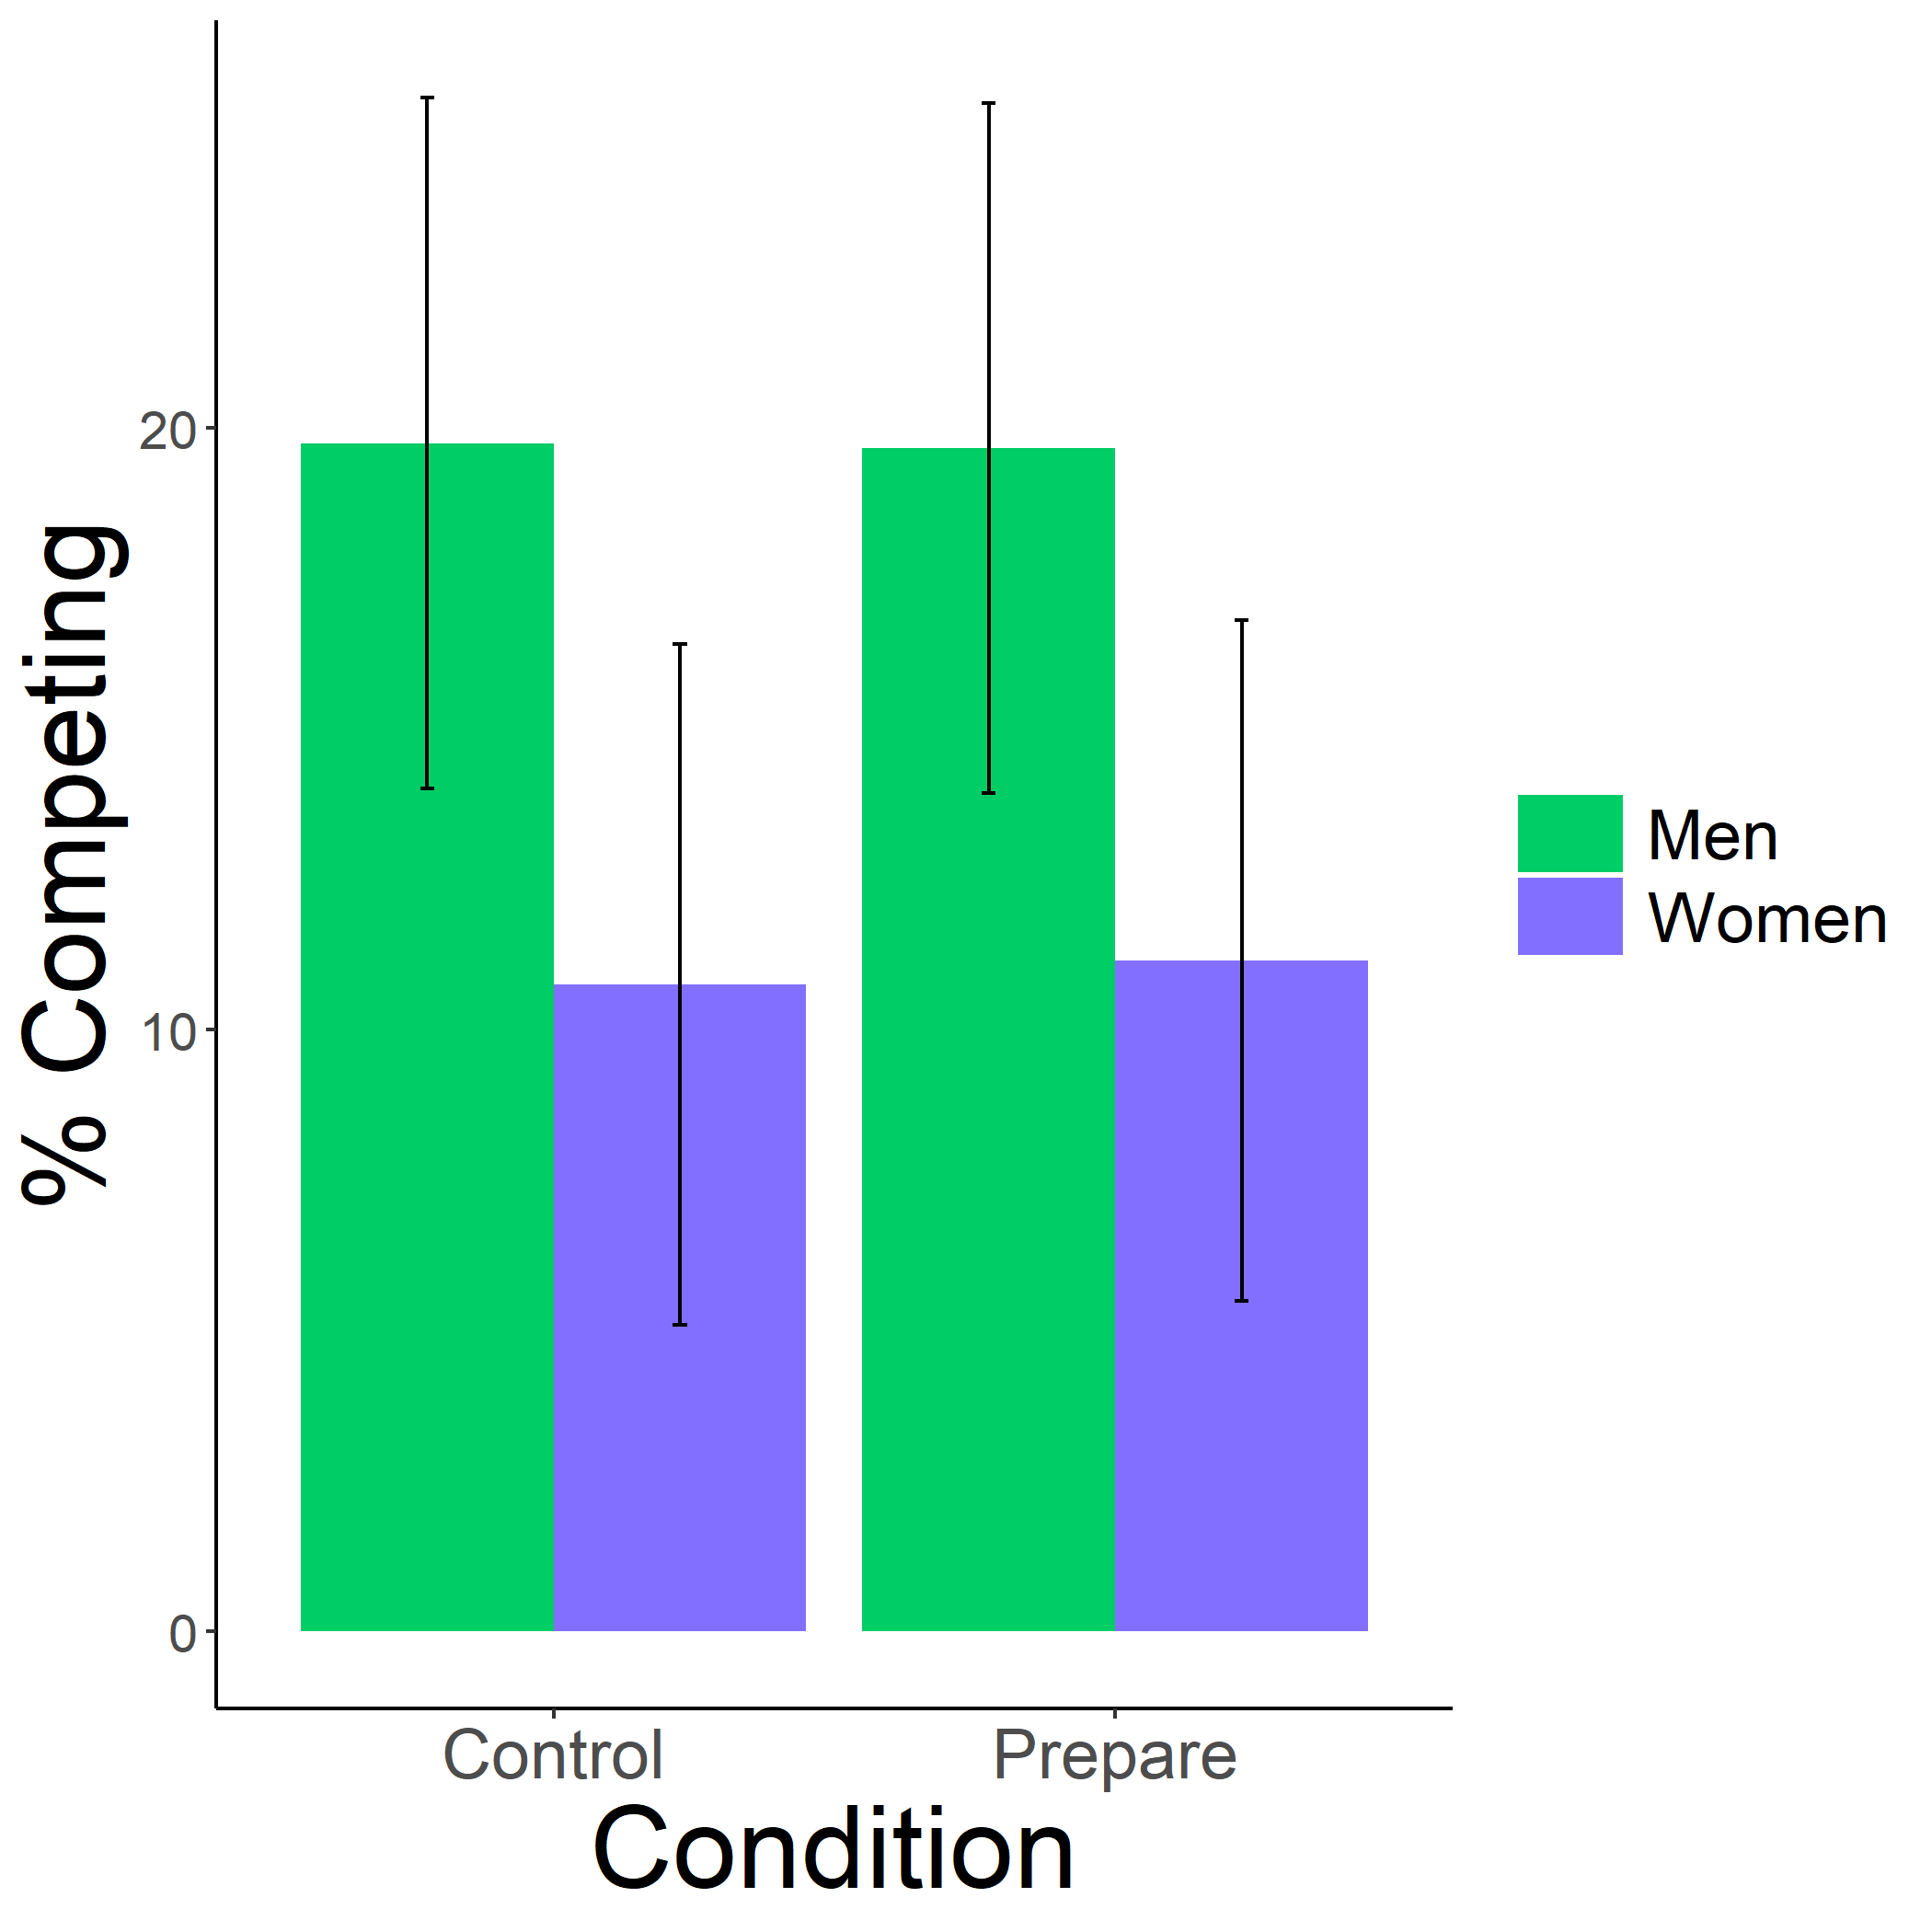
\includegraphics[width=29.17in]{C:/Users/keana/OneDrive - PennO365/Comp_transfer2018/Penn/practice_study/gender-practice/study1/figs/fig00_comp-choice-by-gender-and-cond-bar} \caption{Proportion of men and women who chose to compete by condition. Error bars represent standard errors.}\label{fig:s100}
\end{figure}

\begin{figure}
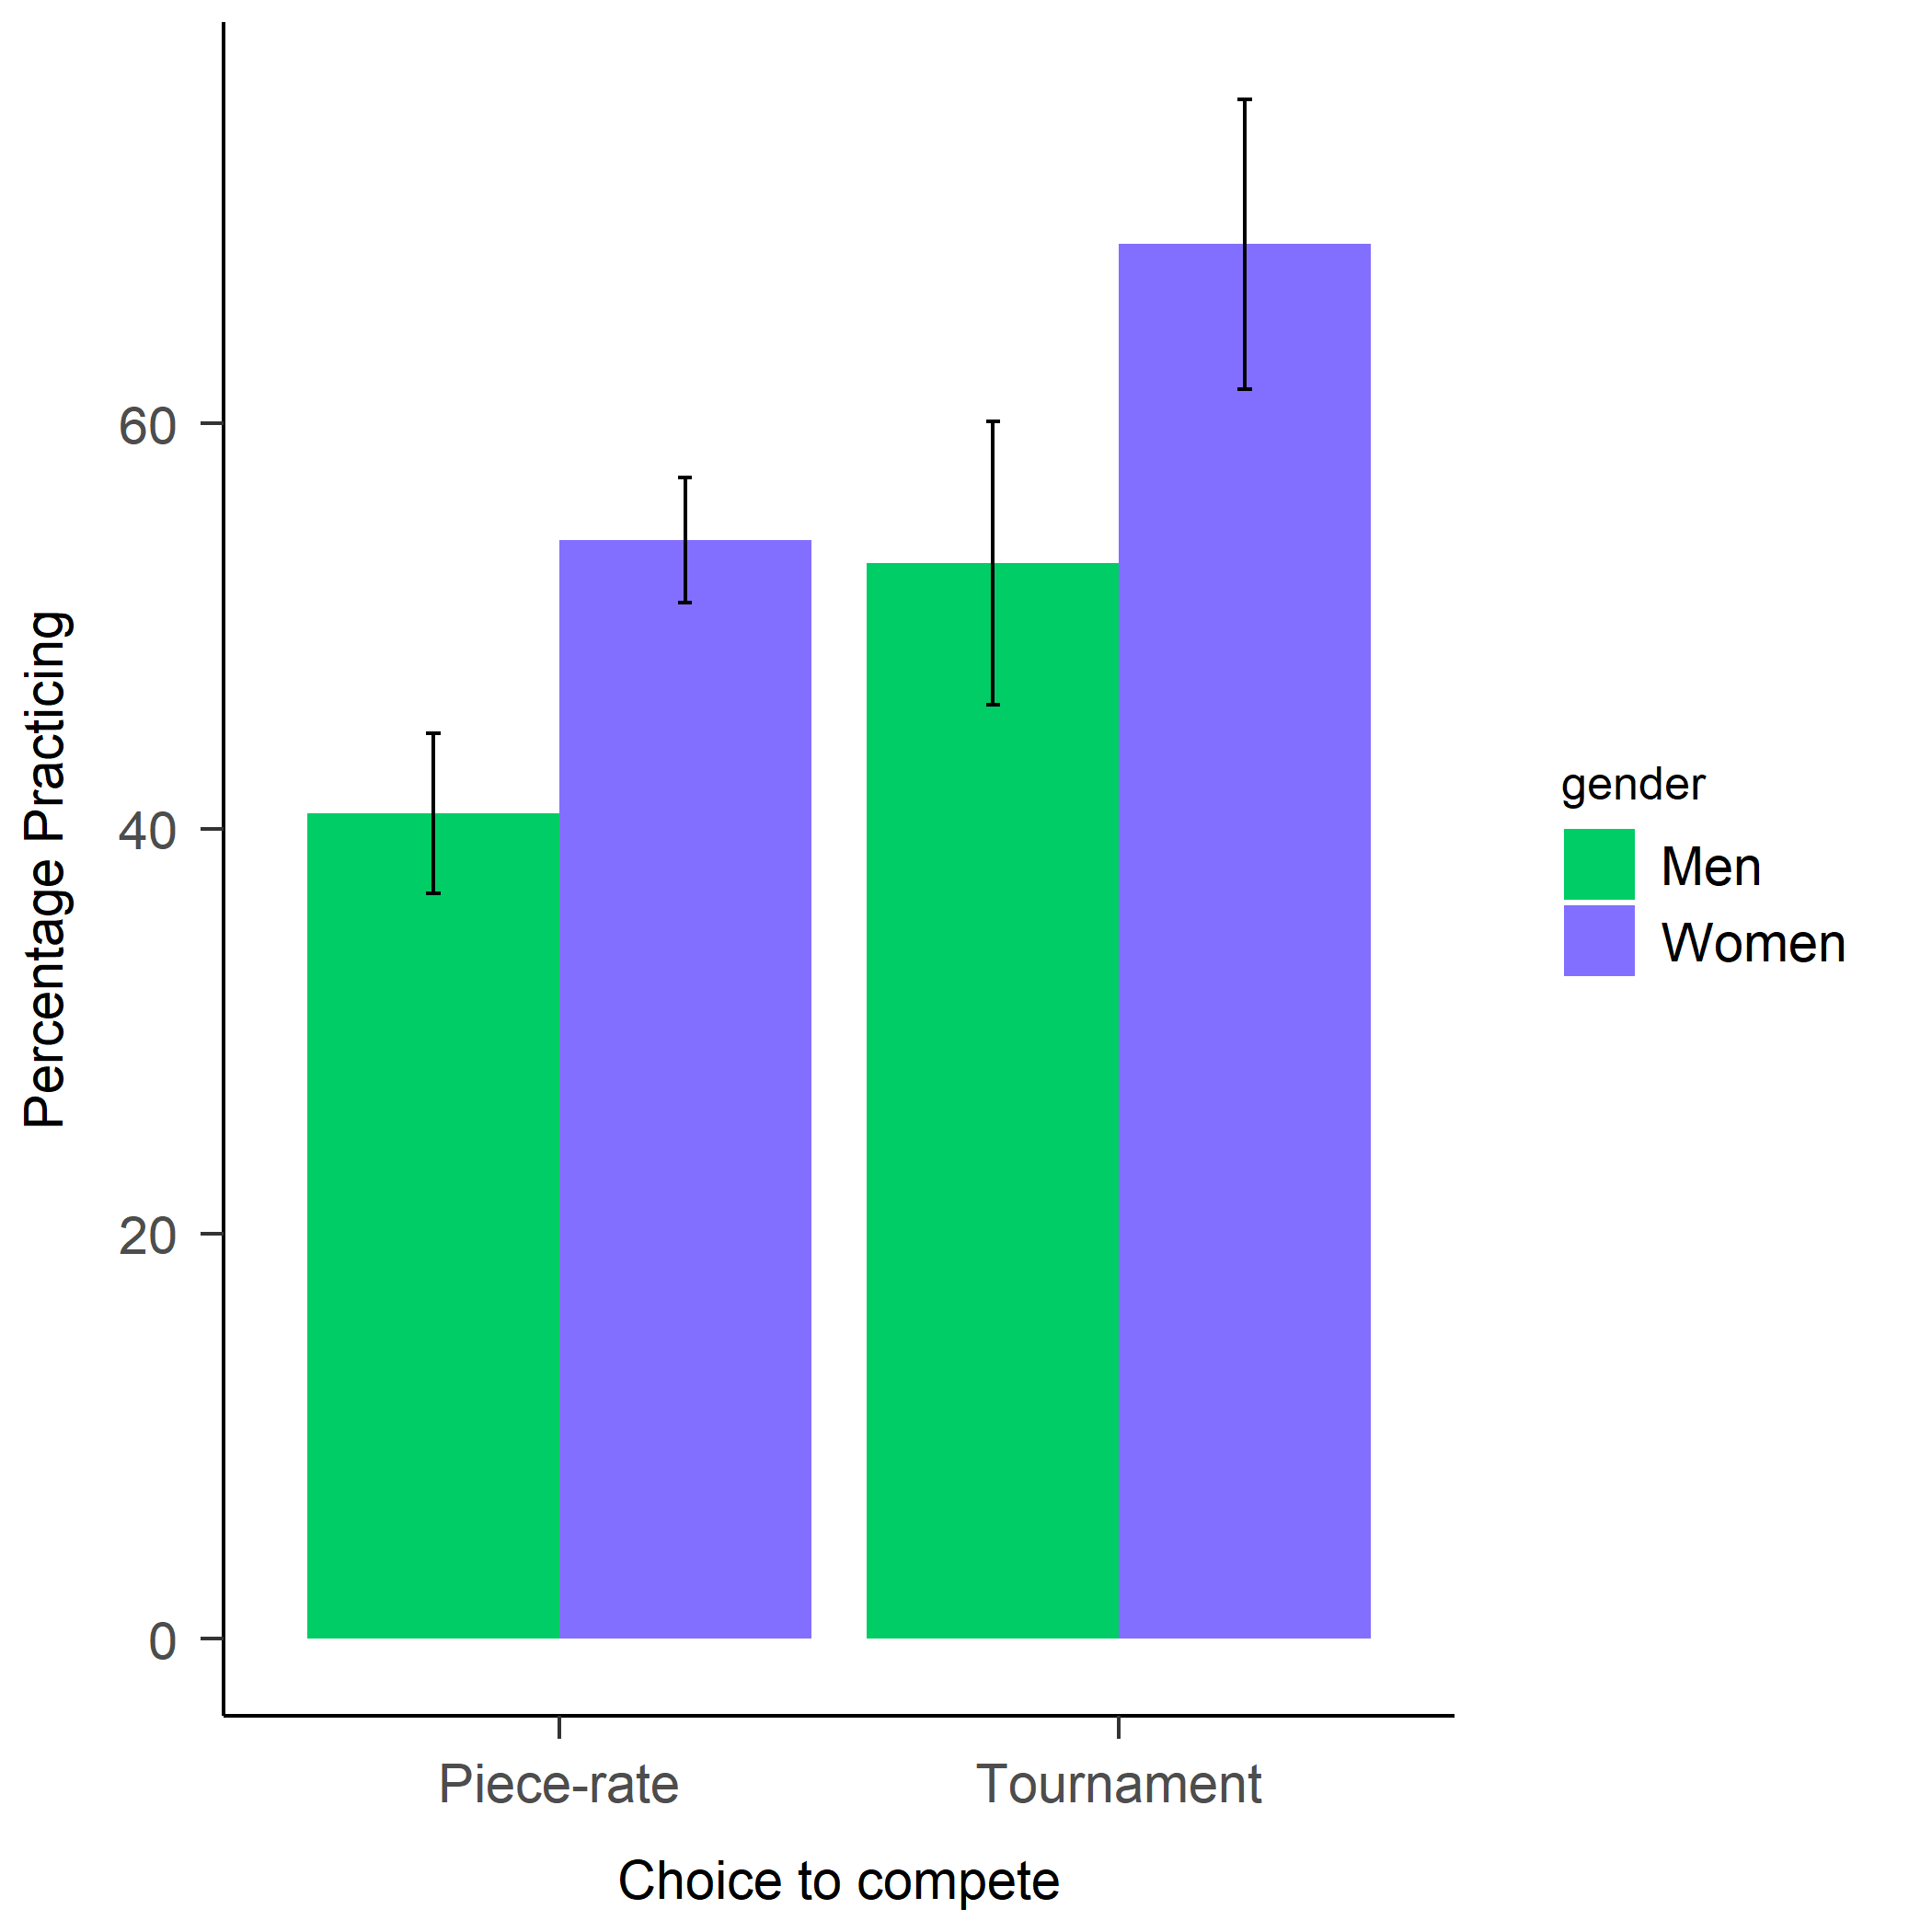
\includegraphics[width=29.17in]{C:/Users/keana/OneDrive - PennO365/Comp_transfer2018/Penn/practice_study/gender-practice/study1/figs/fig01_pract-choice-by-gender-and-comp-choice-bar} \caption{Proportion of men and women who chose to prepare by choice to compete. Error bars represent standard errors.}\label{fig:s101}
\end{figure}

\begin{figure}
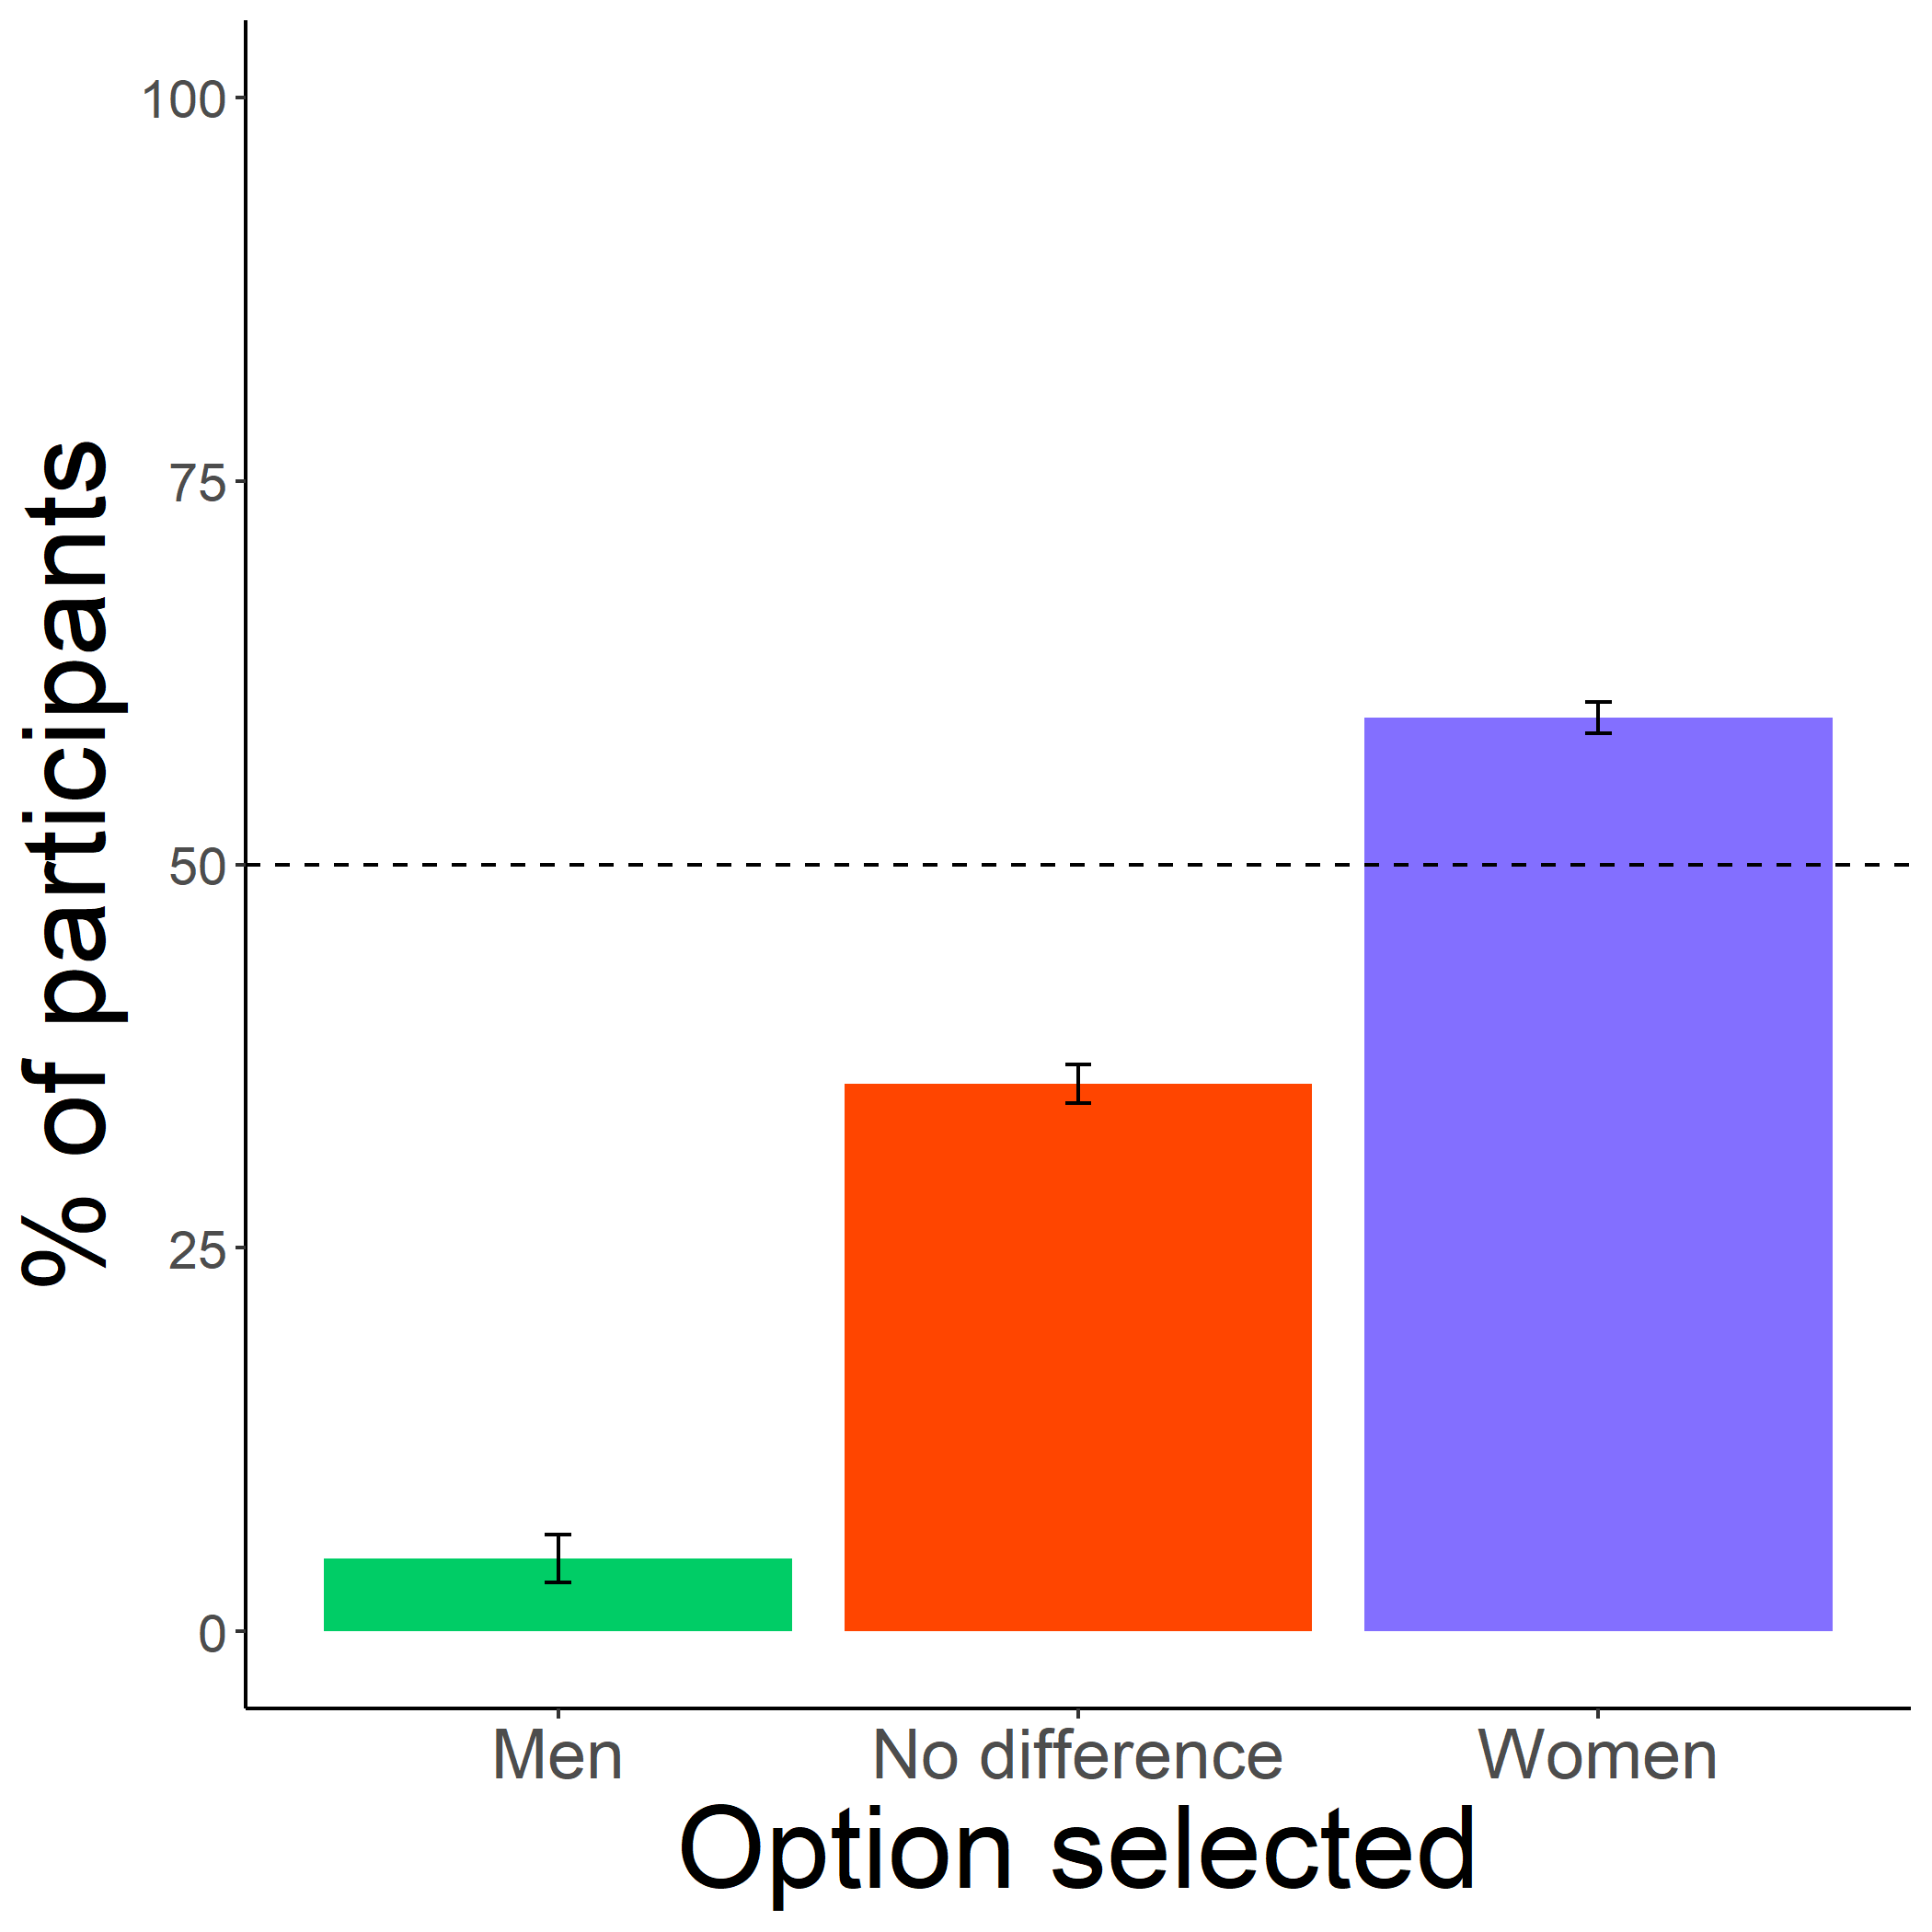
\includegraphics[width=29.17in]{C:/Users/keana/OneDrive - PennO365/Comp_transfer2018/Penn/practice_study/gender-practice/study1/figs/fig03_perc-task-gender-pract} \caption{Participants' perceptions of gender differences in the choice to practice on the task. Error bars represent standard errors.}\label{fig:s103}
\end{figure}

\begin{figure}
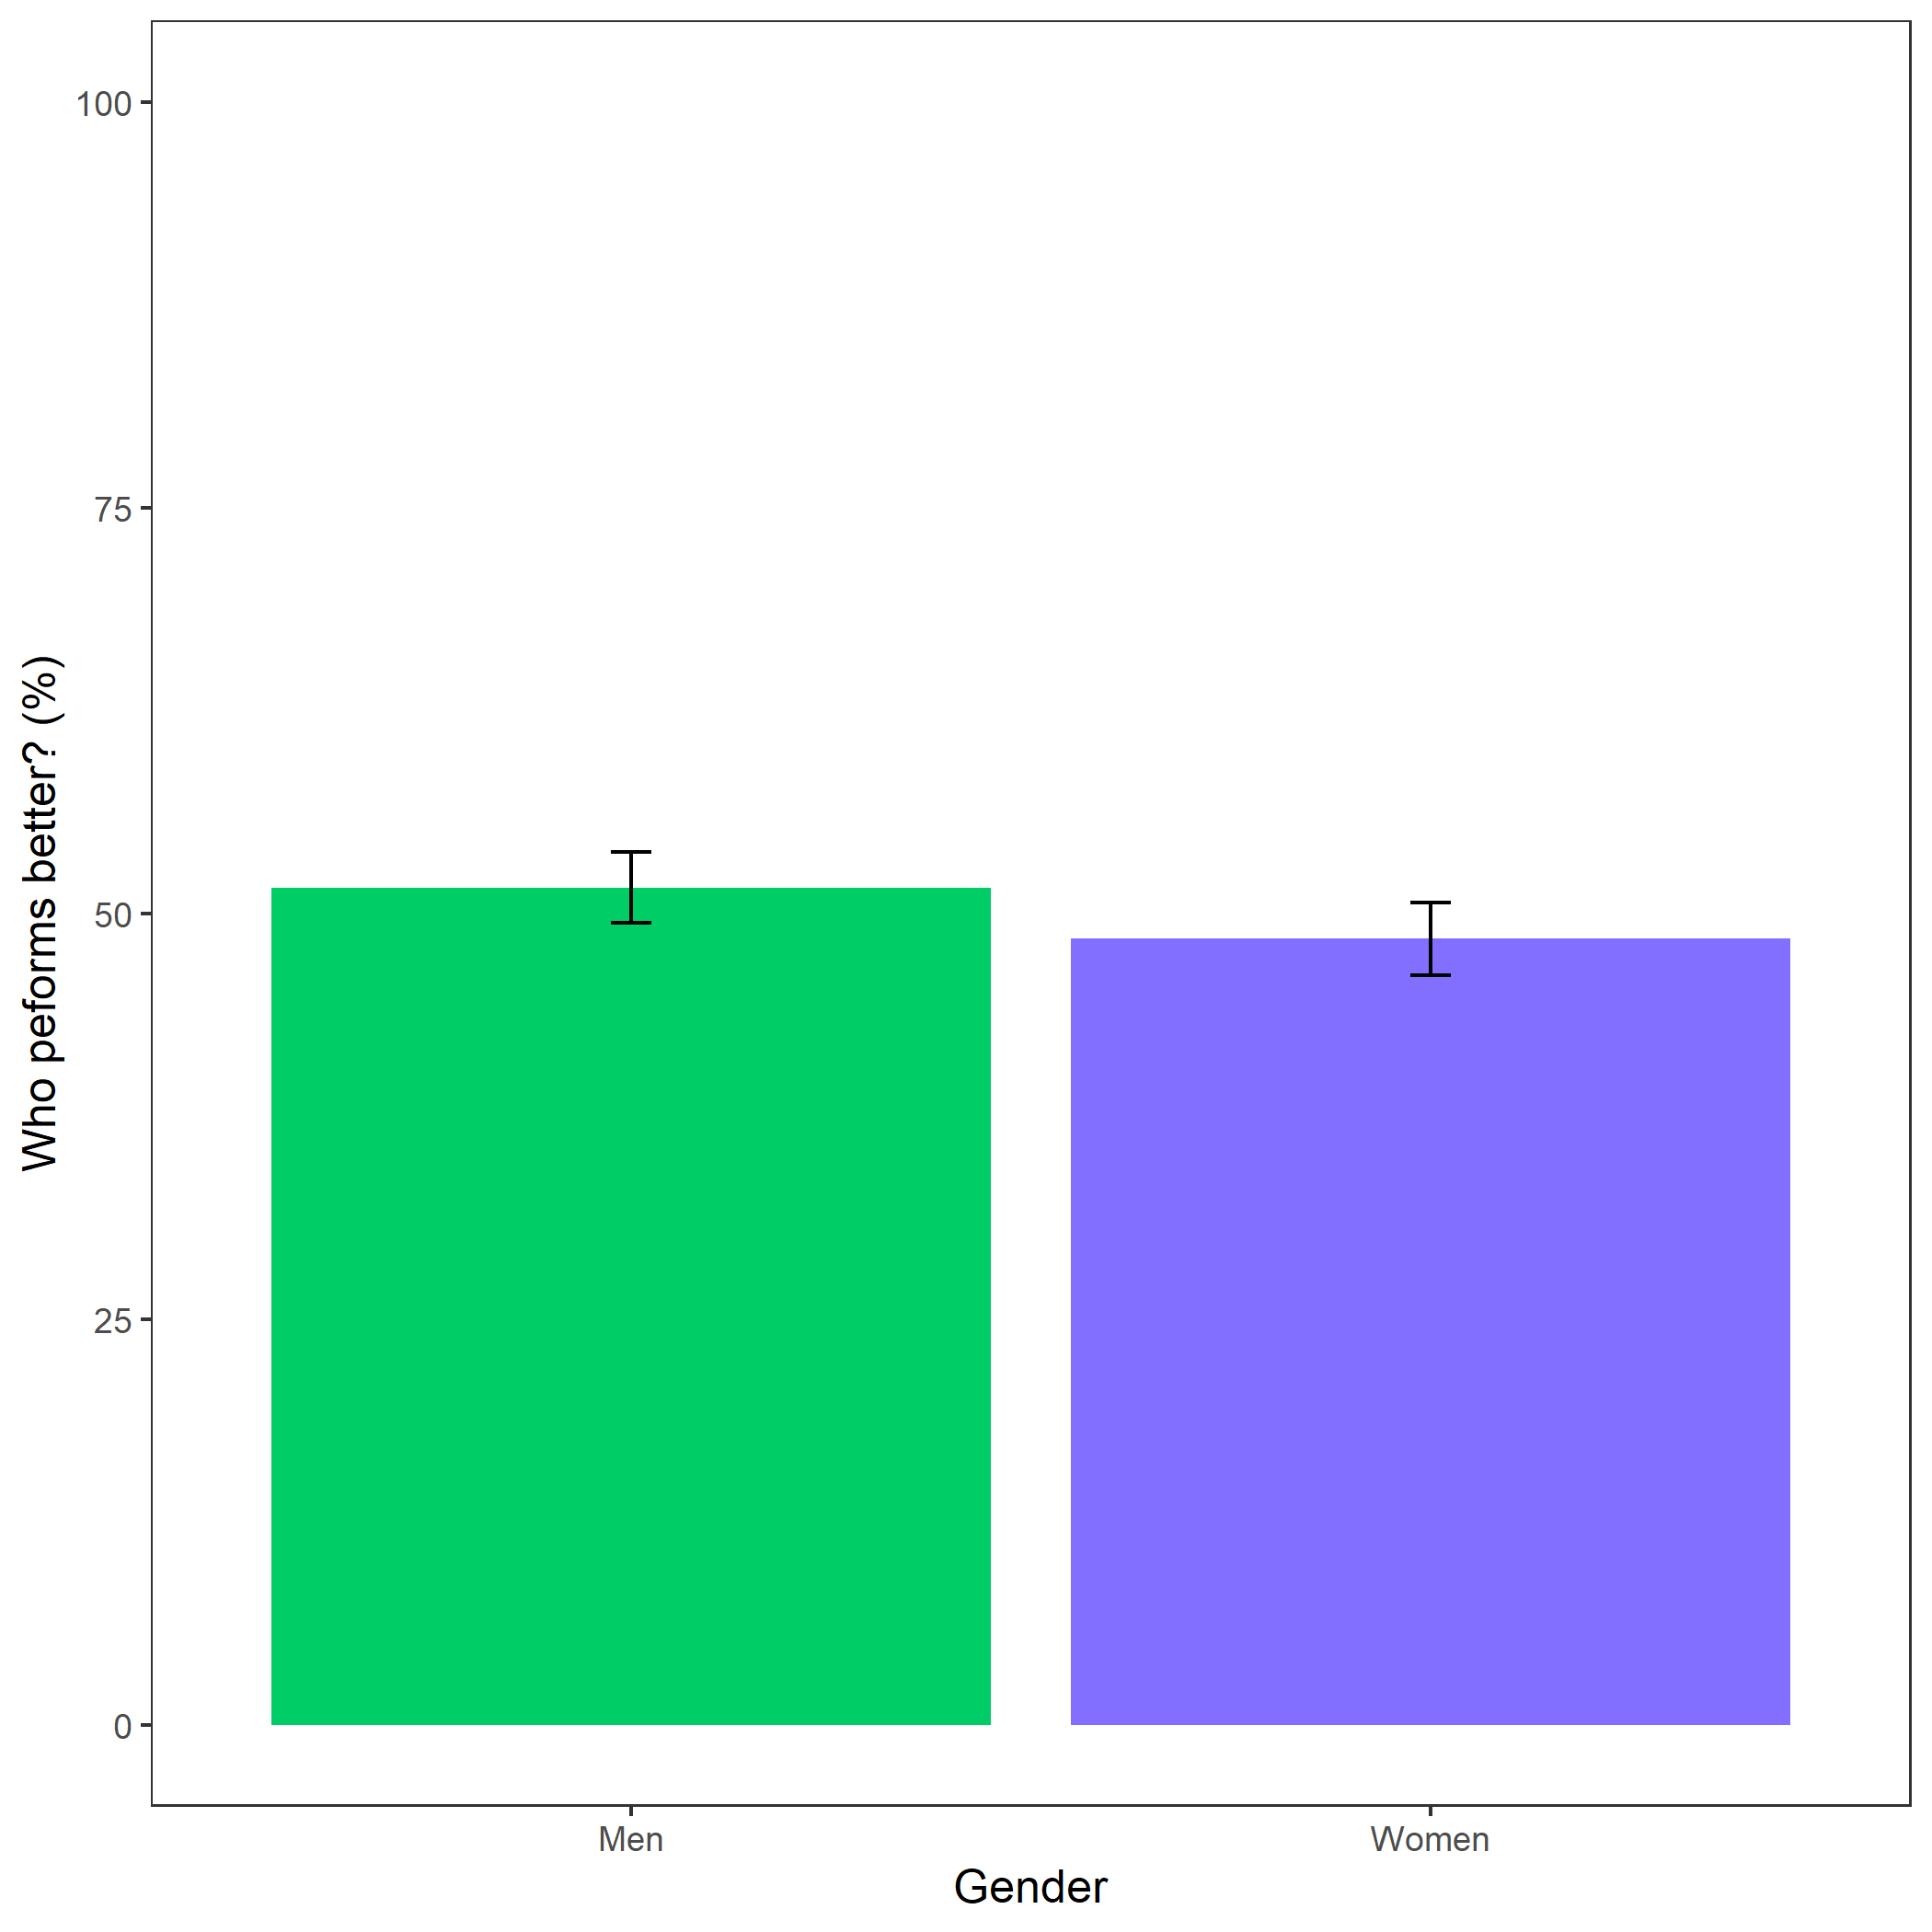
\includegraphics[width=29.17in]{C:/Users/keana/OneDrive - PennO365/Comp_transfer2018/Penn/practice_study/gender-practice/study1/figs/fig04_better-gender-guess} \caption{Participants' perceptions of gender differences in performance on the task. Error bars represent standard errors.}\label{fig:s104}
\end{figure}

\begin{figure}
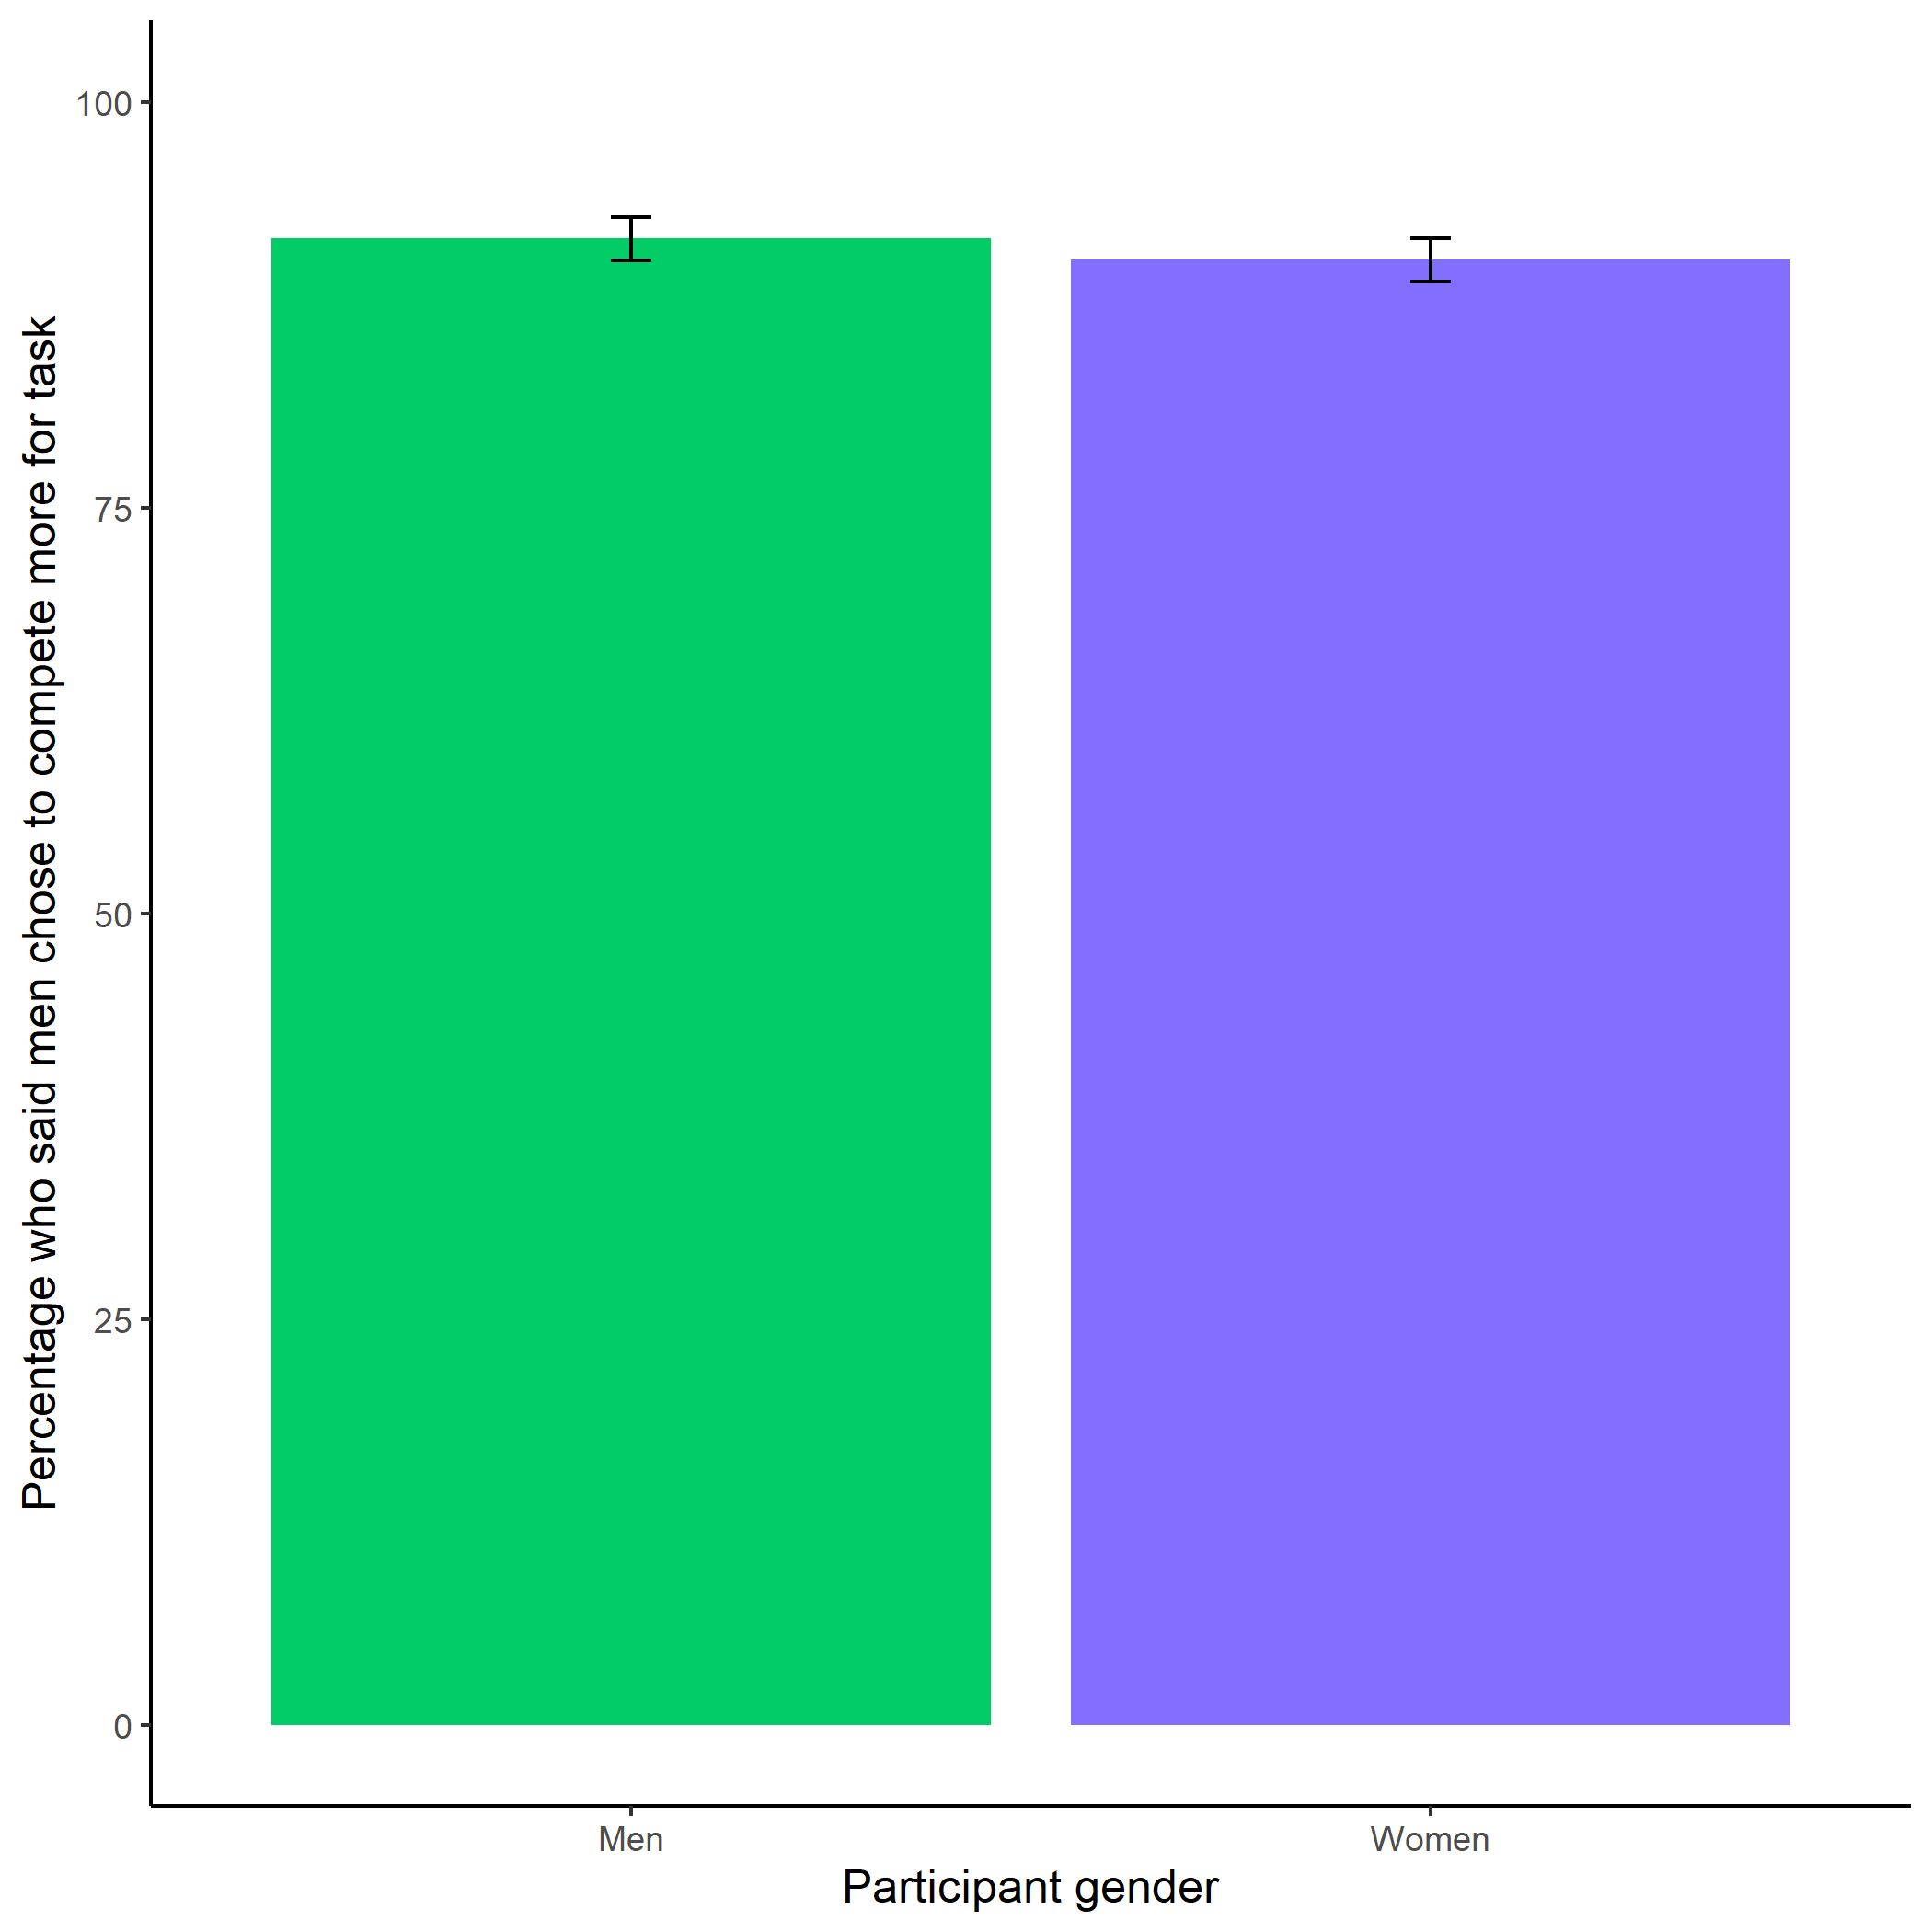
\includegraphics[width=29.17in]{C:/Users/keana/OneDrive - PennO365/Comp_transfer2018/Penn/practice_study/gender-practice/study1/figs/fig05_perc-gender-comp} \caption{Participants' perceptions of gender differences in choice to compete. Error bars represent standard errors.}\label{fig:s105}
\end{figure}

\begin{figure}
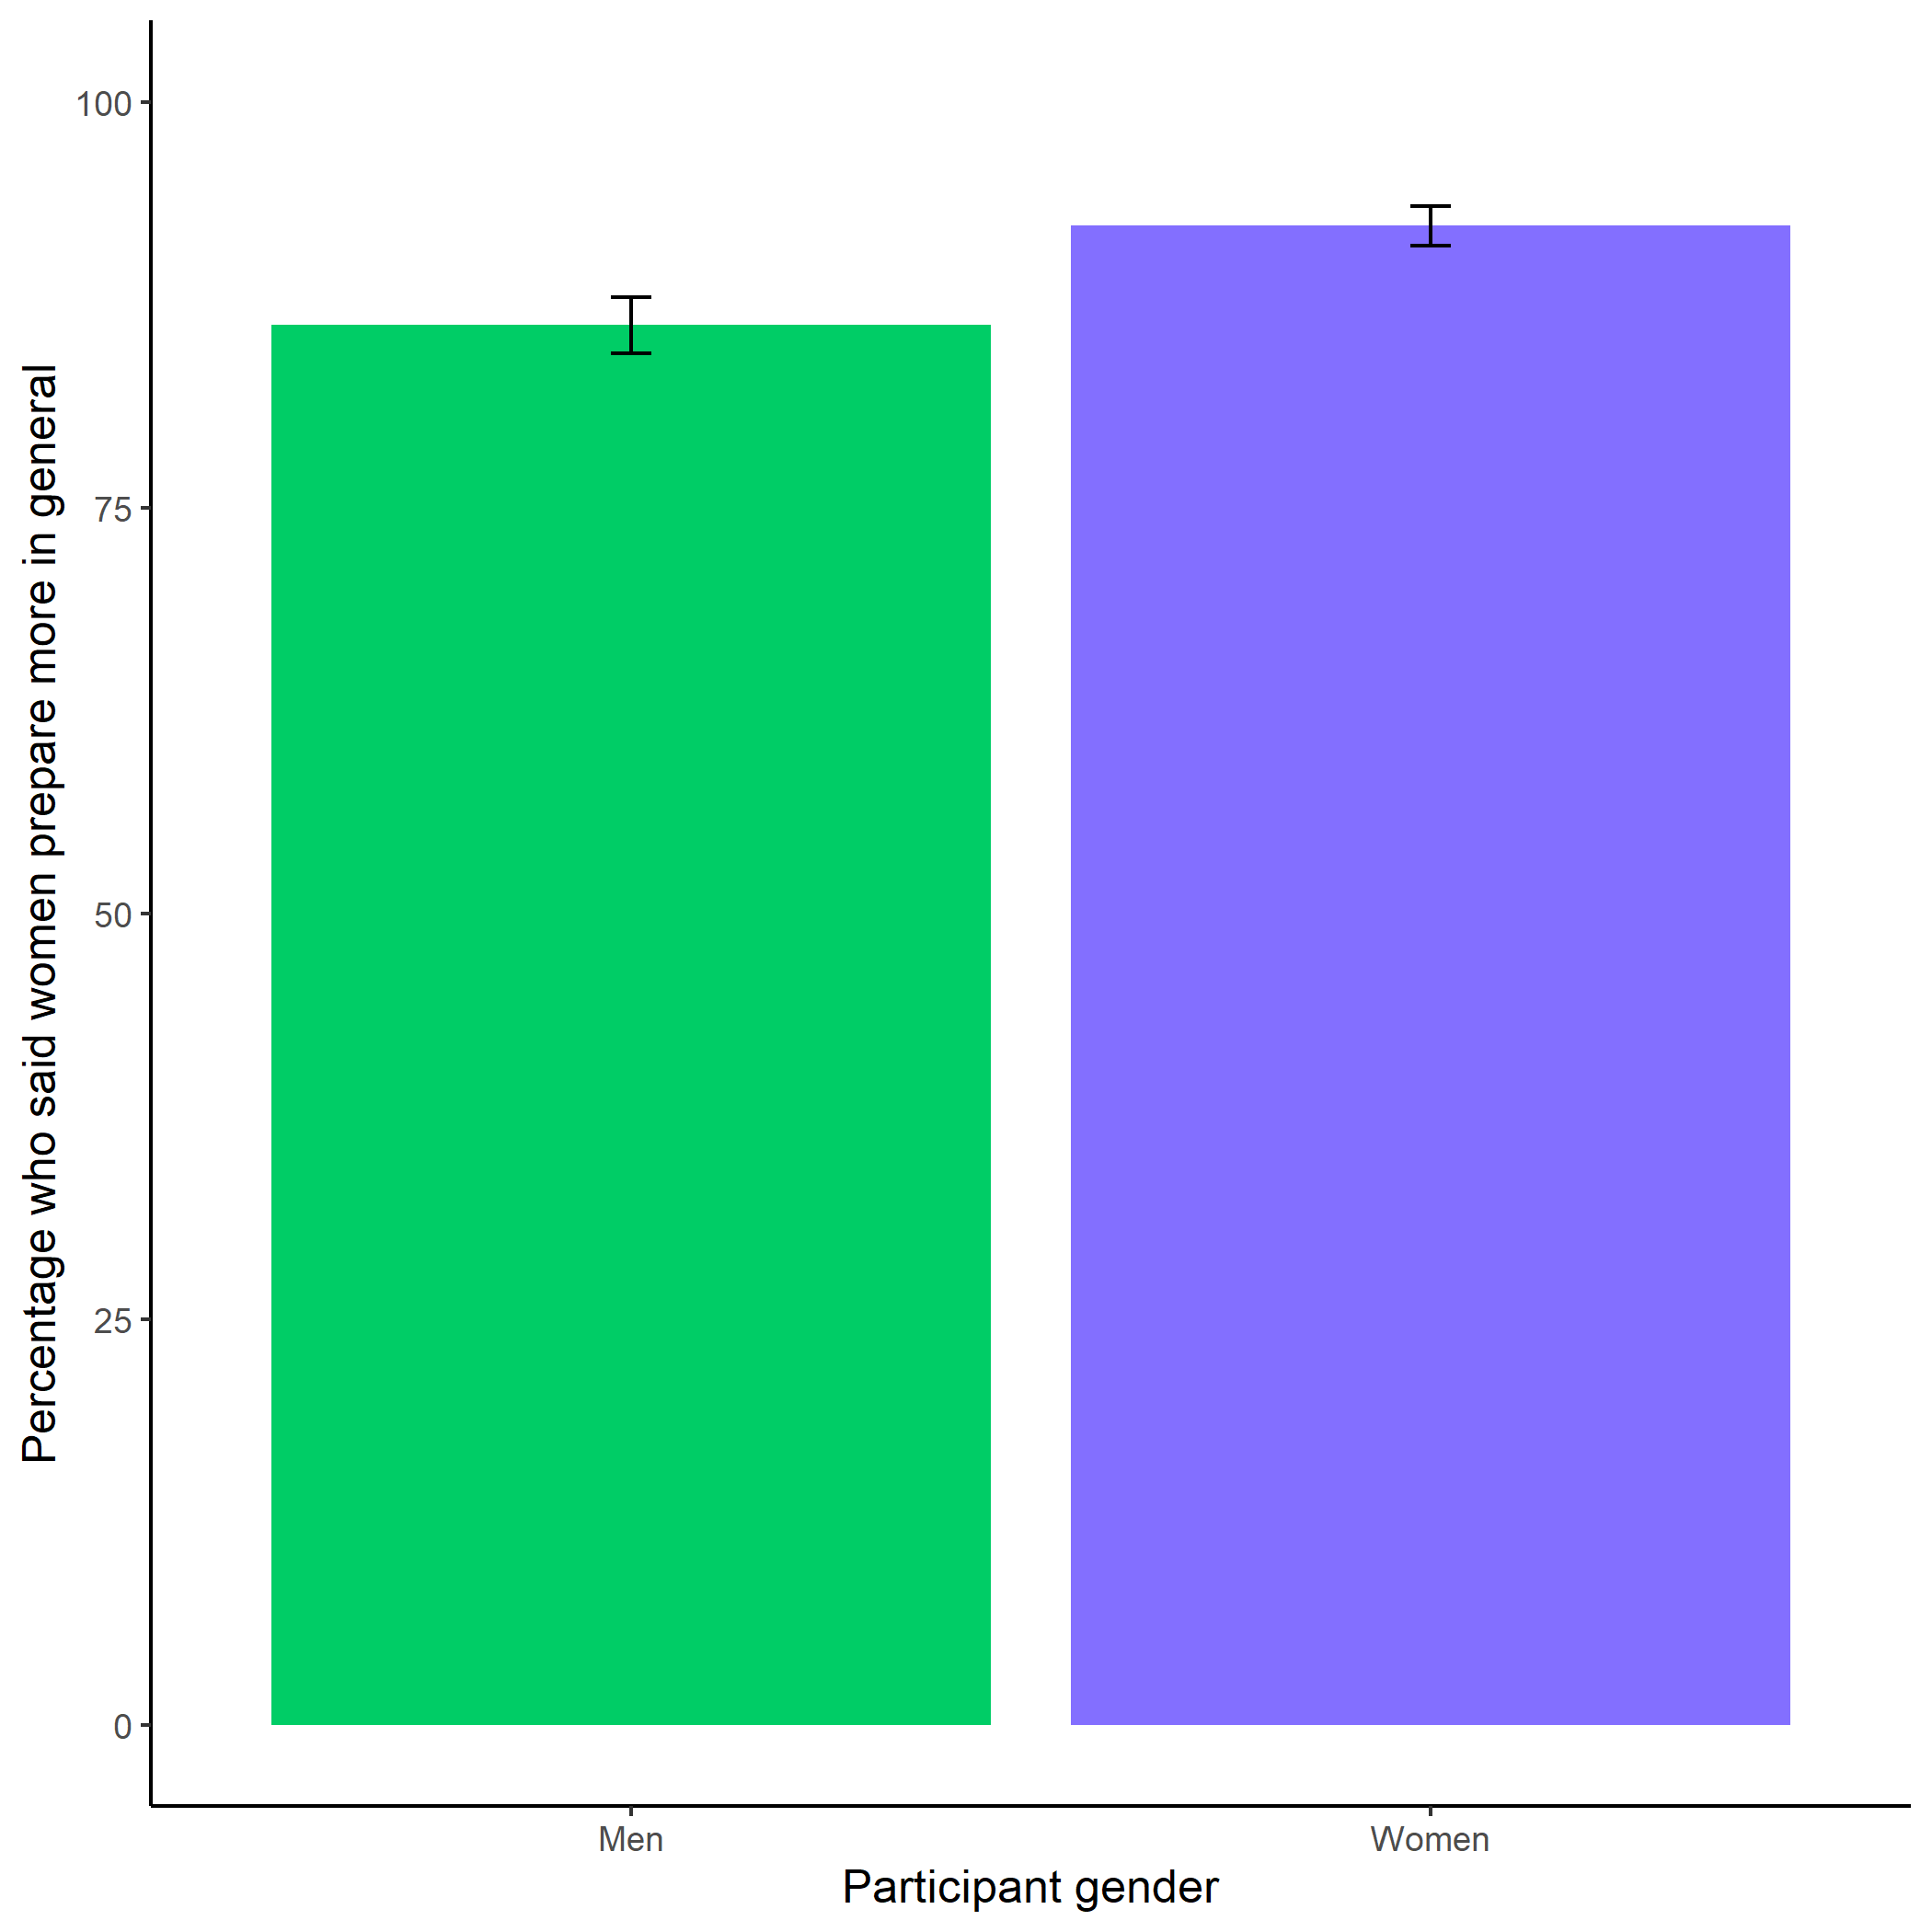
\includegraphics[width=29.17in]{C:/Users/keana/OneDrive - PennO365/Comp_transfer2018/Penn/practice_study/gender-practice/study1/figs/fig06_perc-gen-gender-pract} \caption{Participants' perceptions of general gender differences in choice to practice. Error bars represent standard errors.}\label{fig:s106}
\end{figure}

\begin{figure}
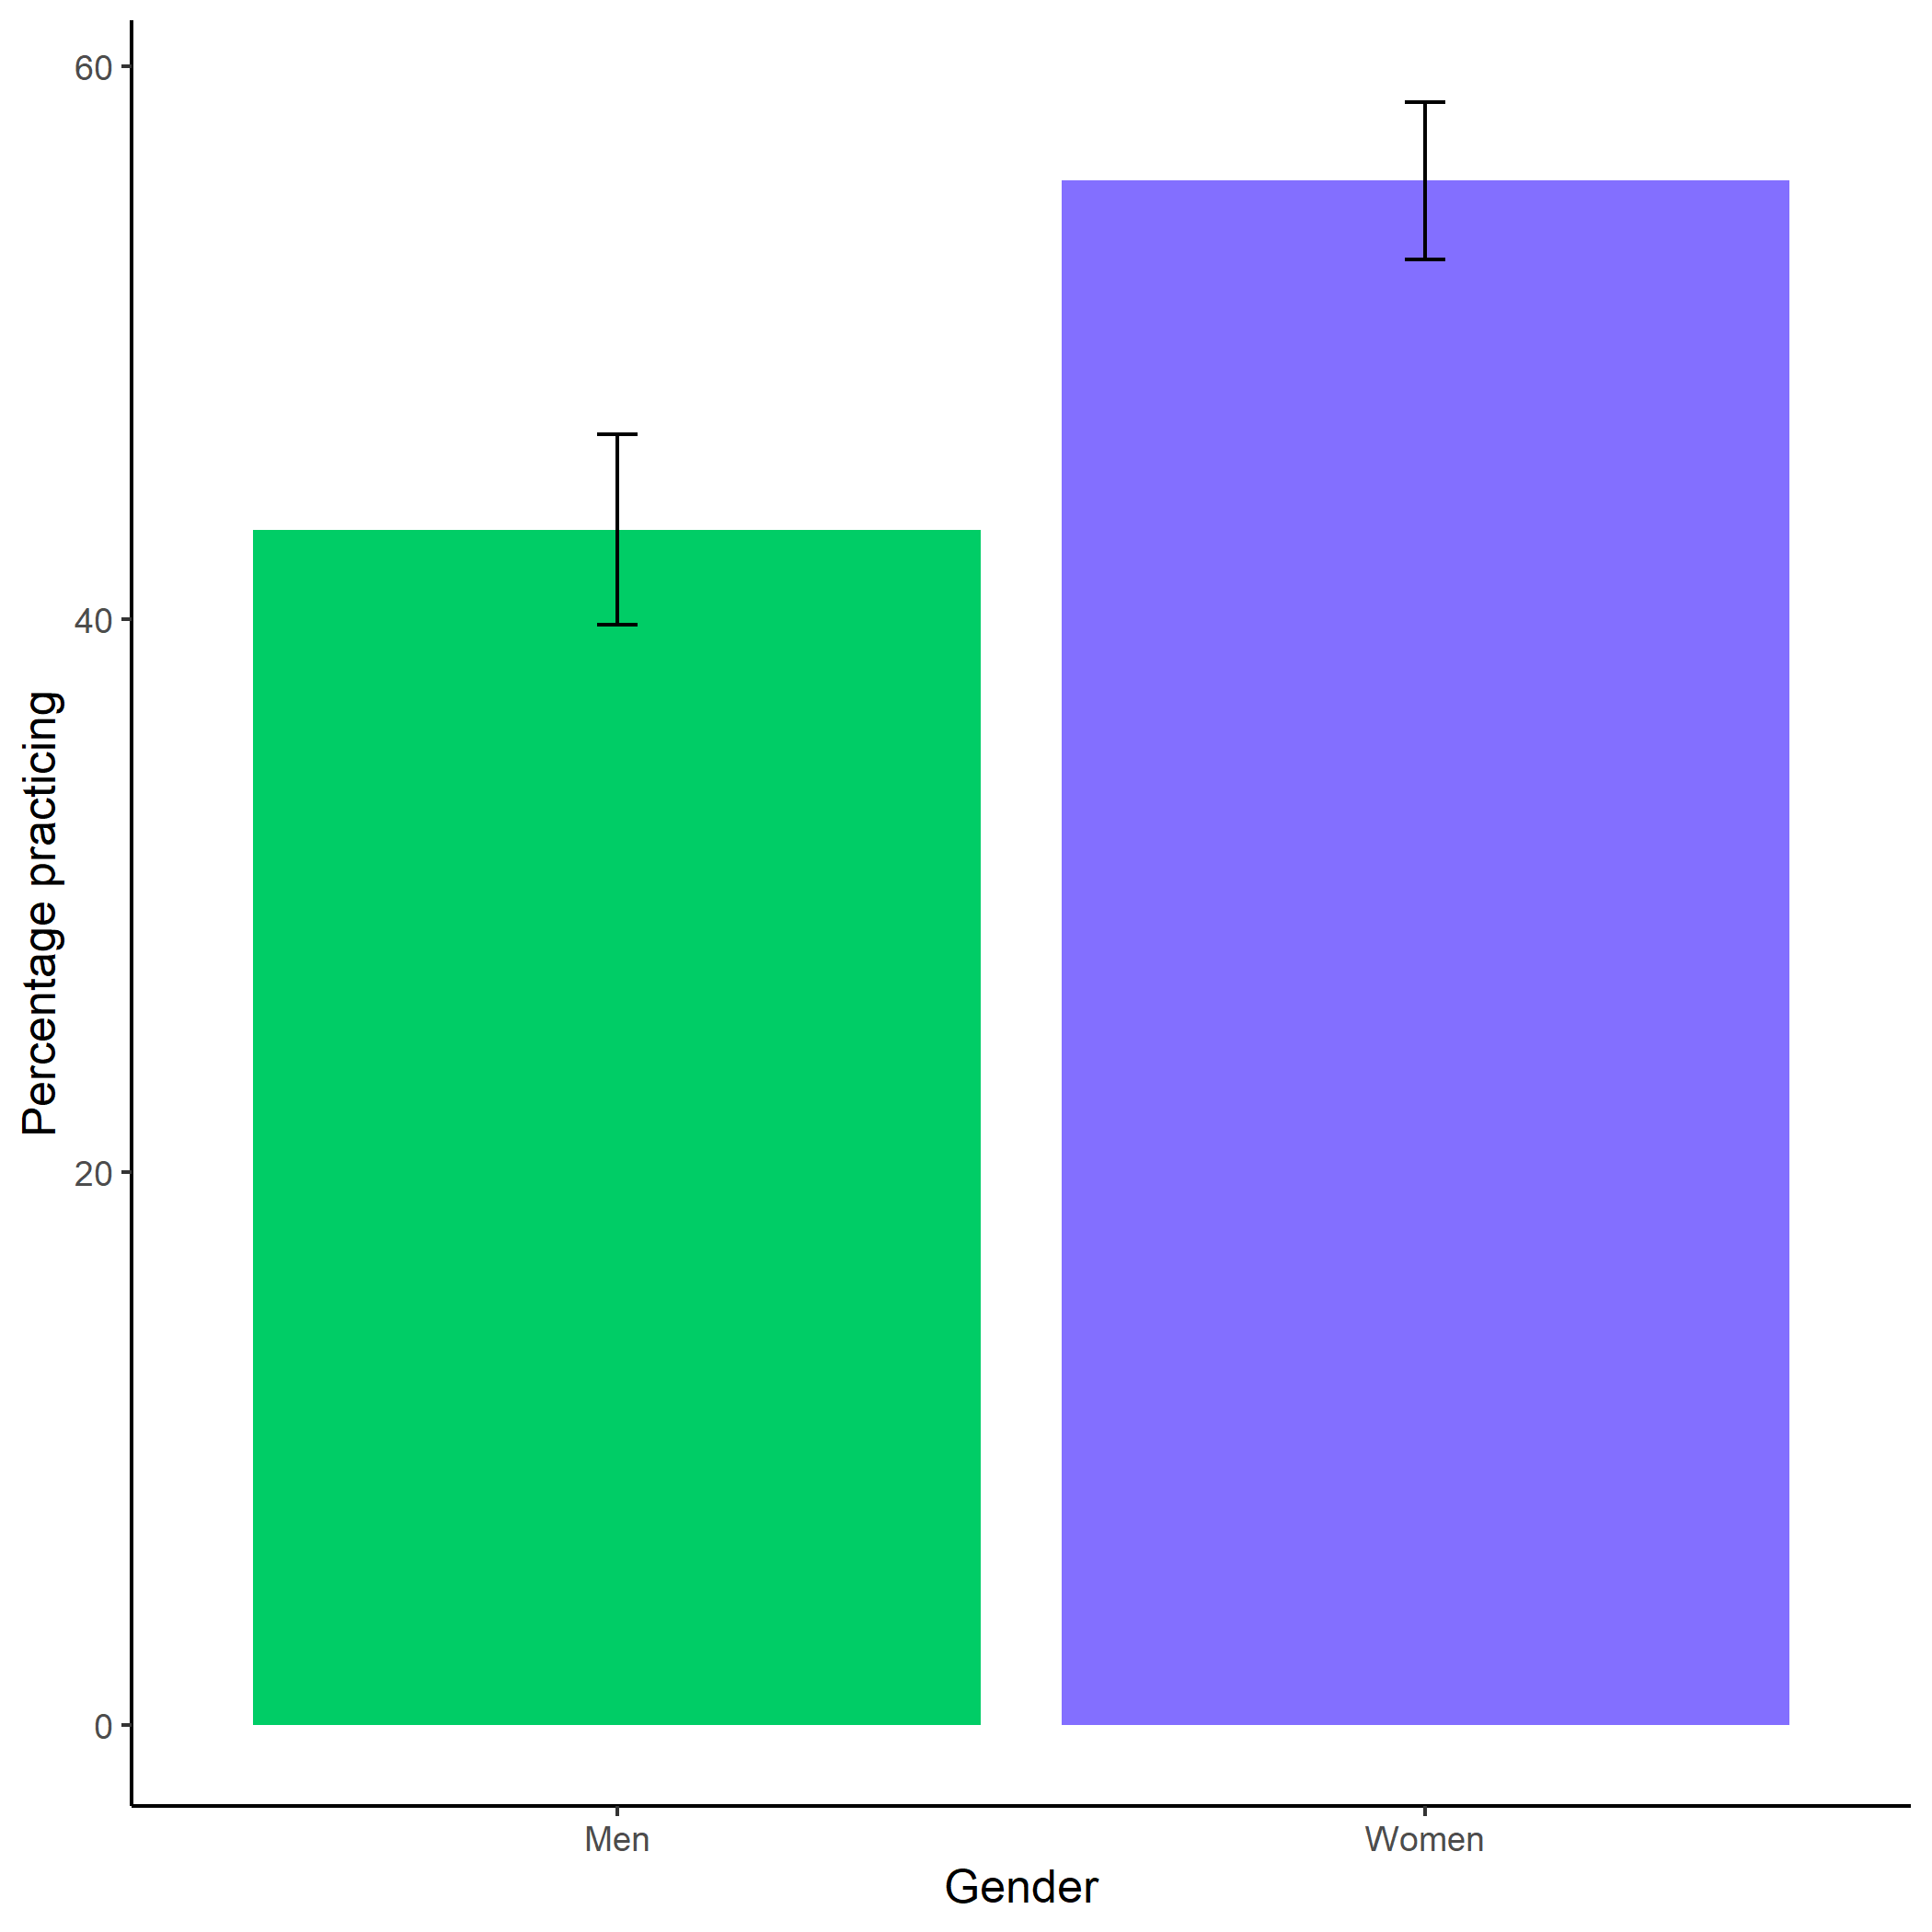
\includegraphics[width=29.17in]{C:/Users/keana/OneDrive - PennO365/Comp_transfer2018/Penn/practice_study/gender-practice/study1/figs/fig07_pract-choice-by-gender} \caption{Participants' perceptions of general gender differences in choice to practice. Error bars represent standard errors.}\label{fig:s107}
\end{figure}

\hypertarget{study-2-1}{%
\section{Study 2}\label{study-2-1}}

\begin{figure}
\includegraphics[width=29.17in]{C:/Users/keana/OneDrive - PennO365/Comp_transfer2018/Penn/practice_study/gender-practice/study2/figs/fig00_comp-choice-women-by-cond} \caption{Proportion of women who chose to compete by condition. We do not find evidence of the hypothesized effect of condition on the choice to compete, there were no significant differences in entry into competition between women in the control vs. prepare conditions. Error bars represent standard errors.}\label{fig:s200}
\end{figure}

\begin{figure}
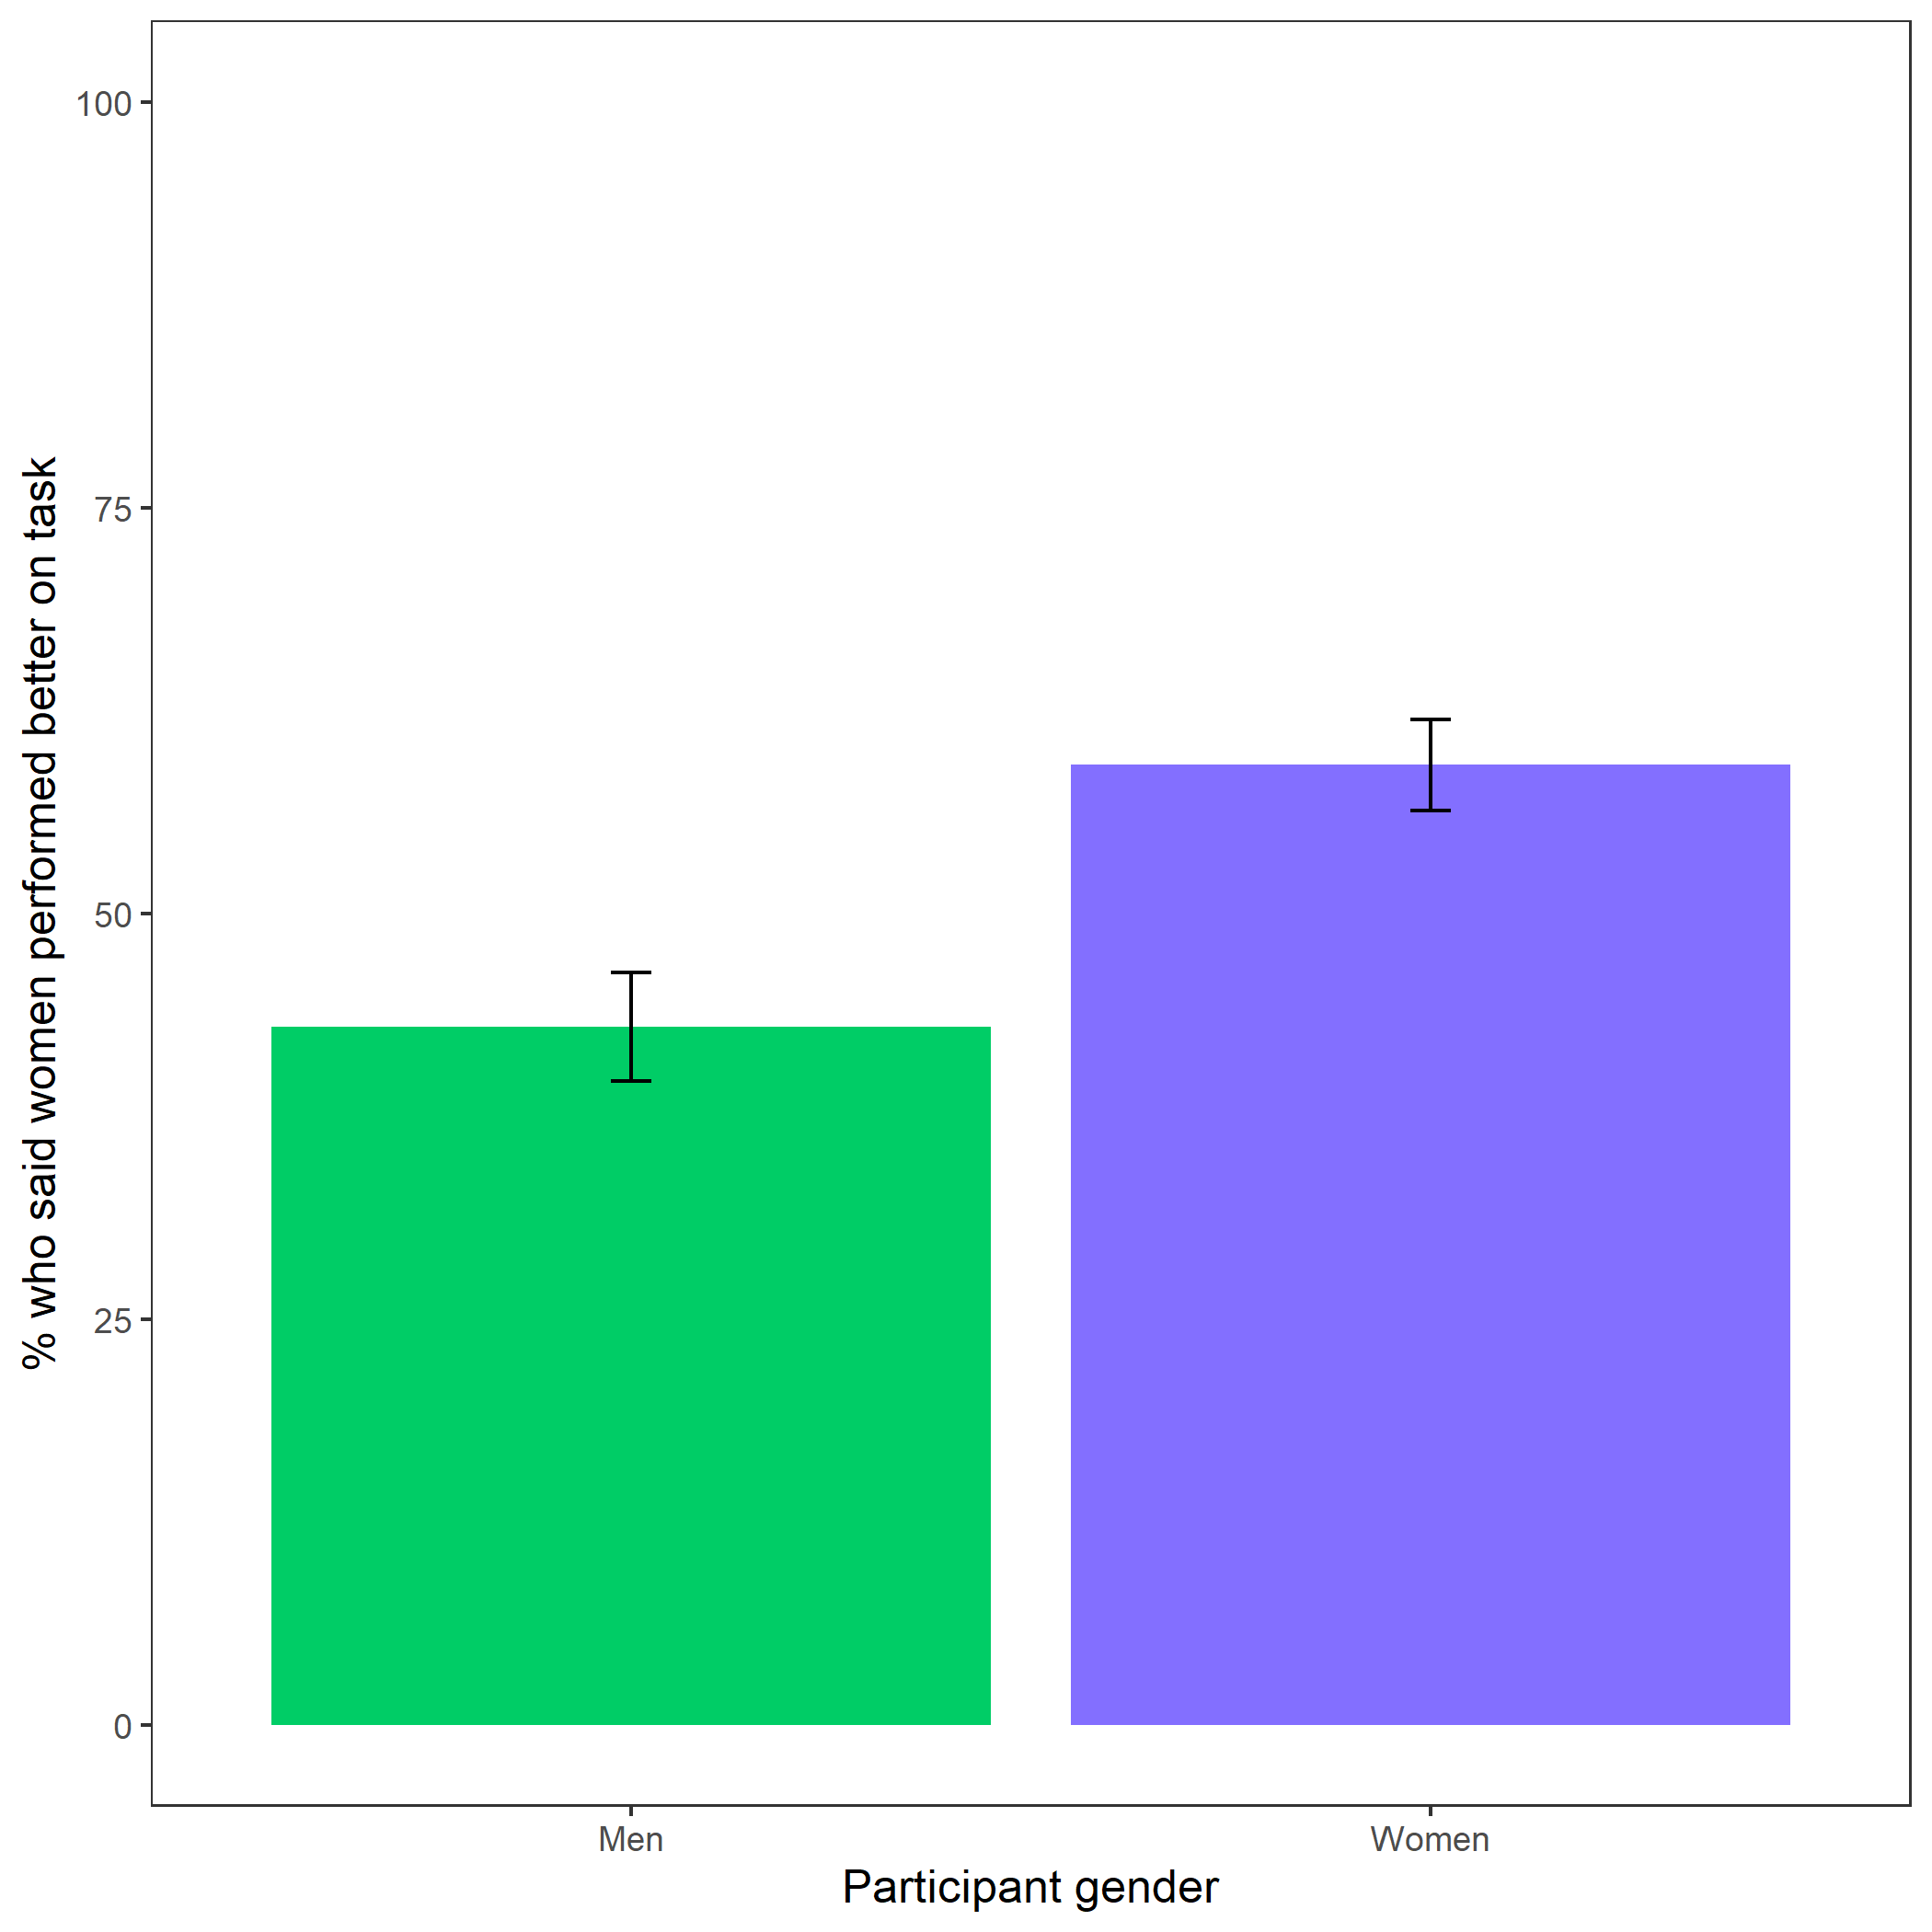
\includegraphics[width=29.17in]{C:/Users/keana/OneDrive - PennO365/Comp_transfer2018/Penn/practice_study/gender-practice/study2/figs/fig01_better-gender-guess} \caption{Participants' perceptions of gender differences in performance on the task. We replicate the effect from Study 1, where participants were not significantly more likely than chance to anticipate that one gender would perform better on the task. Error bars represent standard errors.}\label{fig:s201}
\end{figure}

\begin{figure}
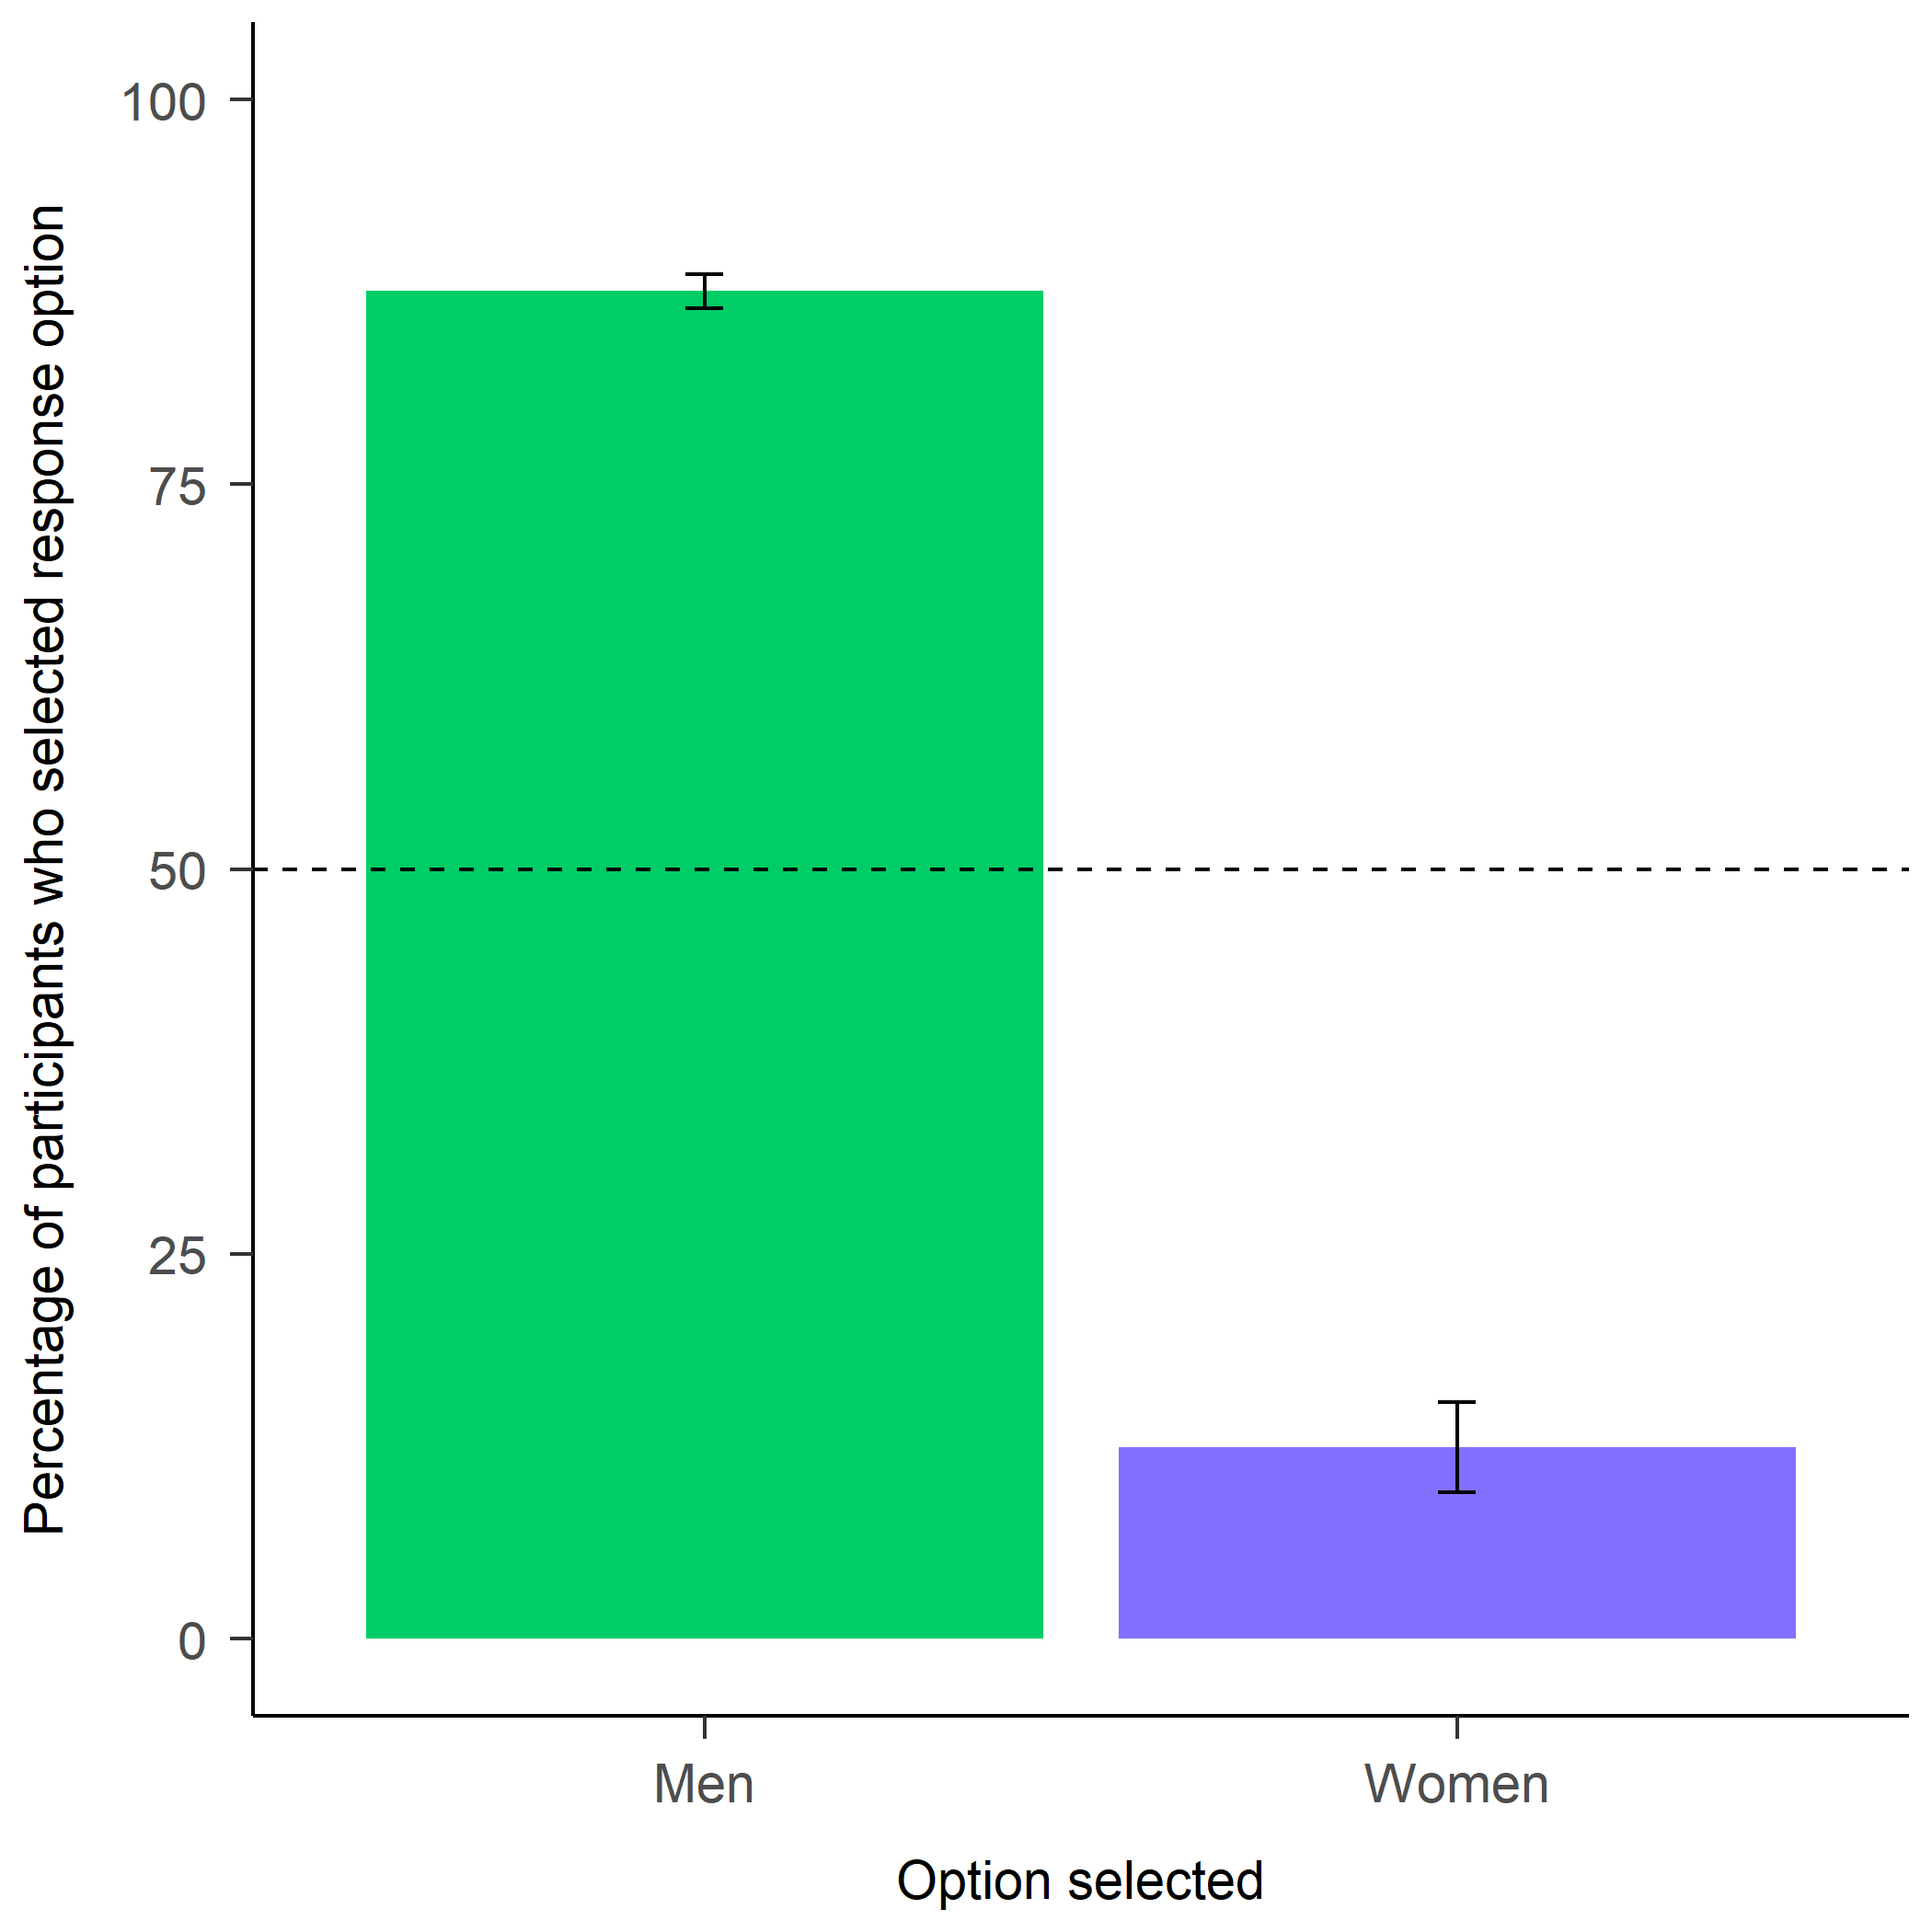
\includegraphics[width=29.17in]{C:/Users/keana/OneDrive - PennO365/Comp_transfer2018/Penn/practice_study/gender-practice/study2/figs/fig02_perc-gender-comp} \caption{Participants' perceptions of gender differences in choice to compete. Replicating the finding from Study 1, participants (especially men) in Study 2 are significantly more likely than chance to state that men chose the competitive payment scheme. Error bars represent standard errors.}\label{fig:s202}
\end{figure}

\begin{figure}
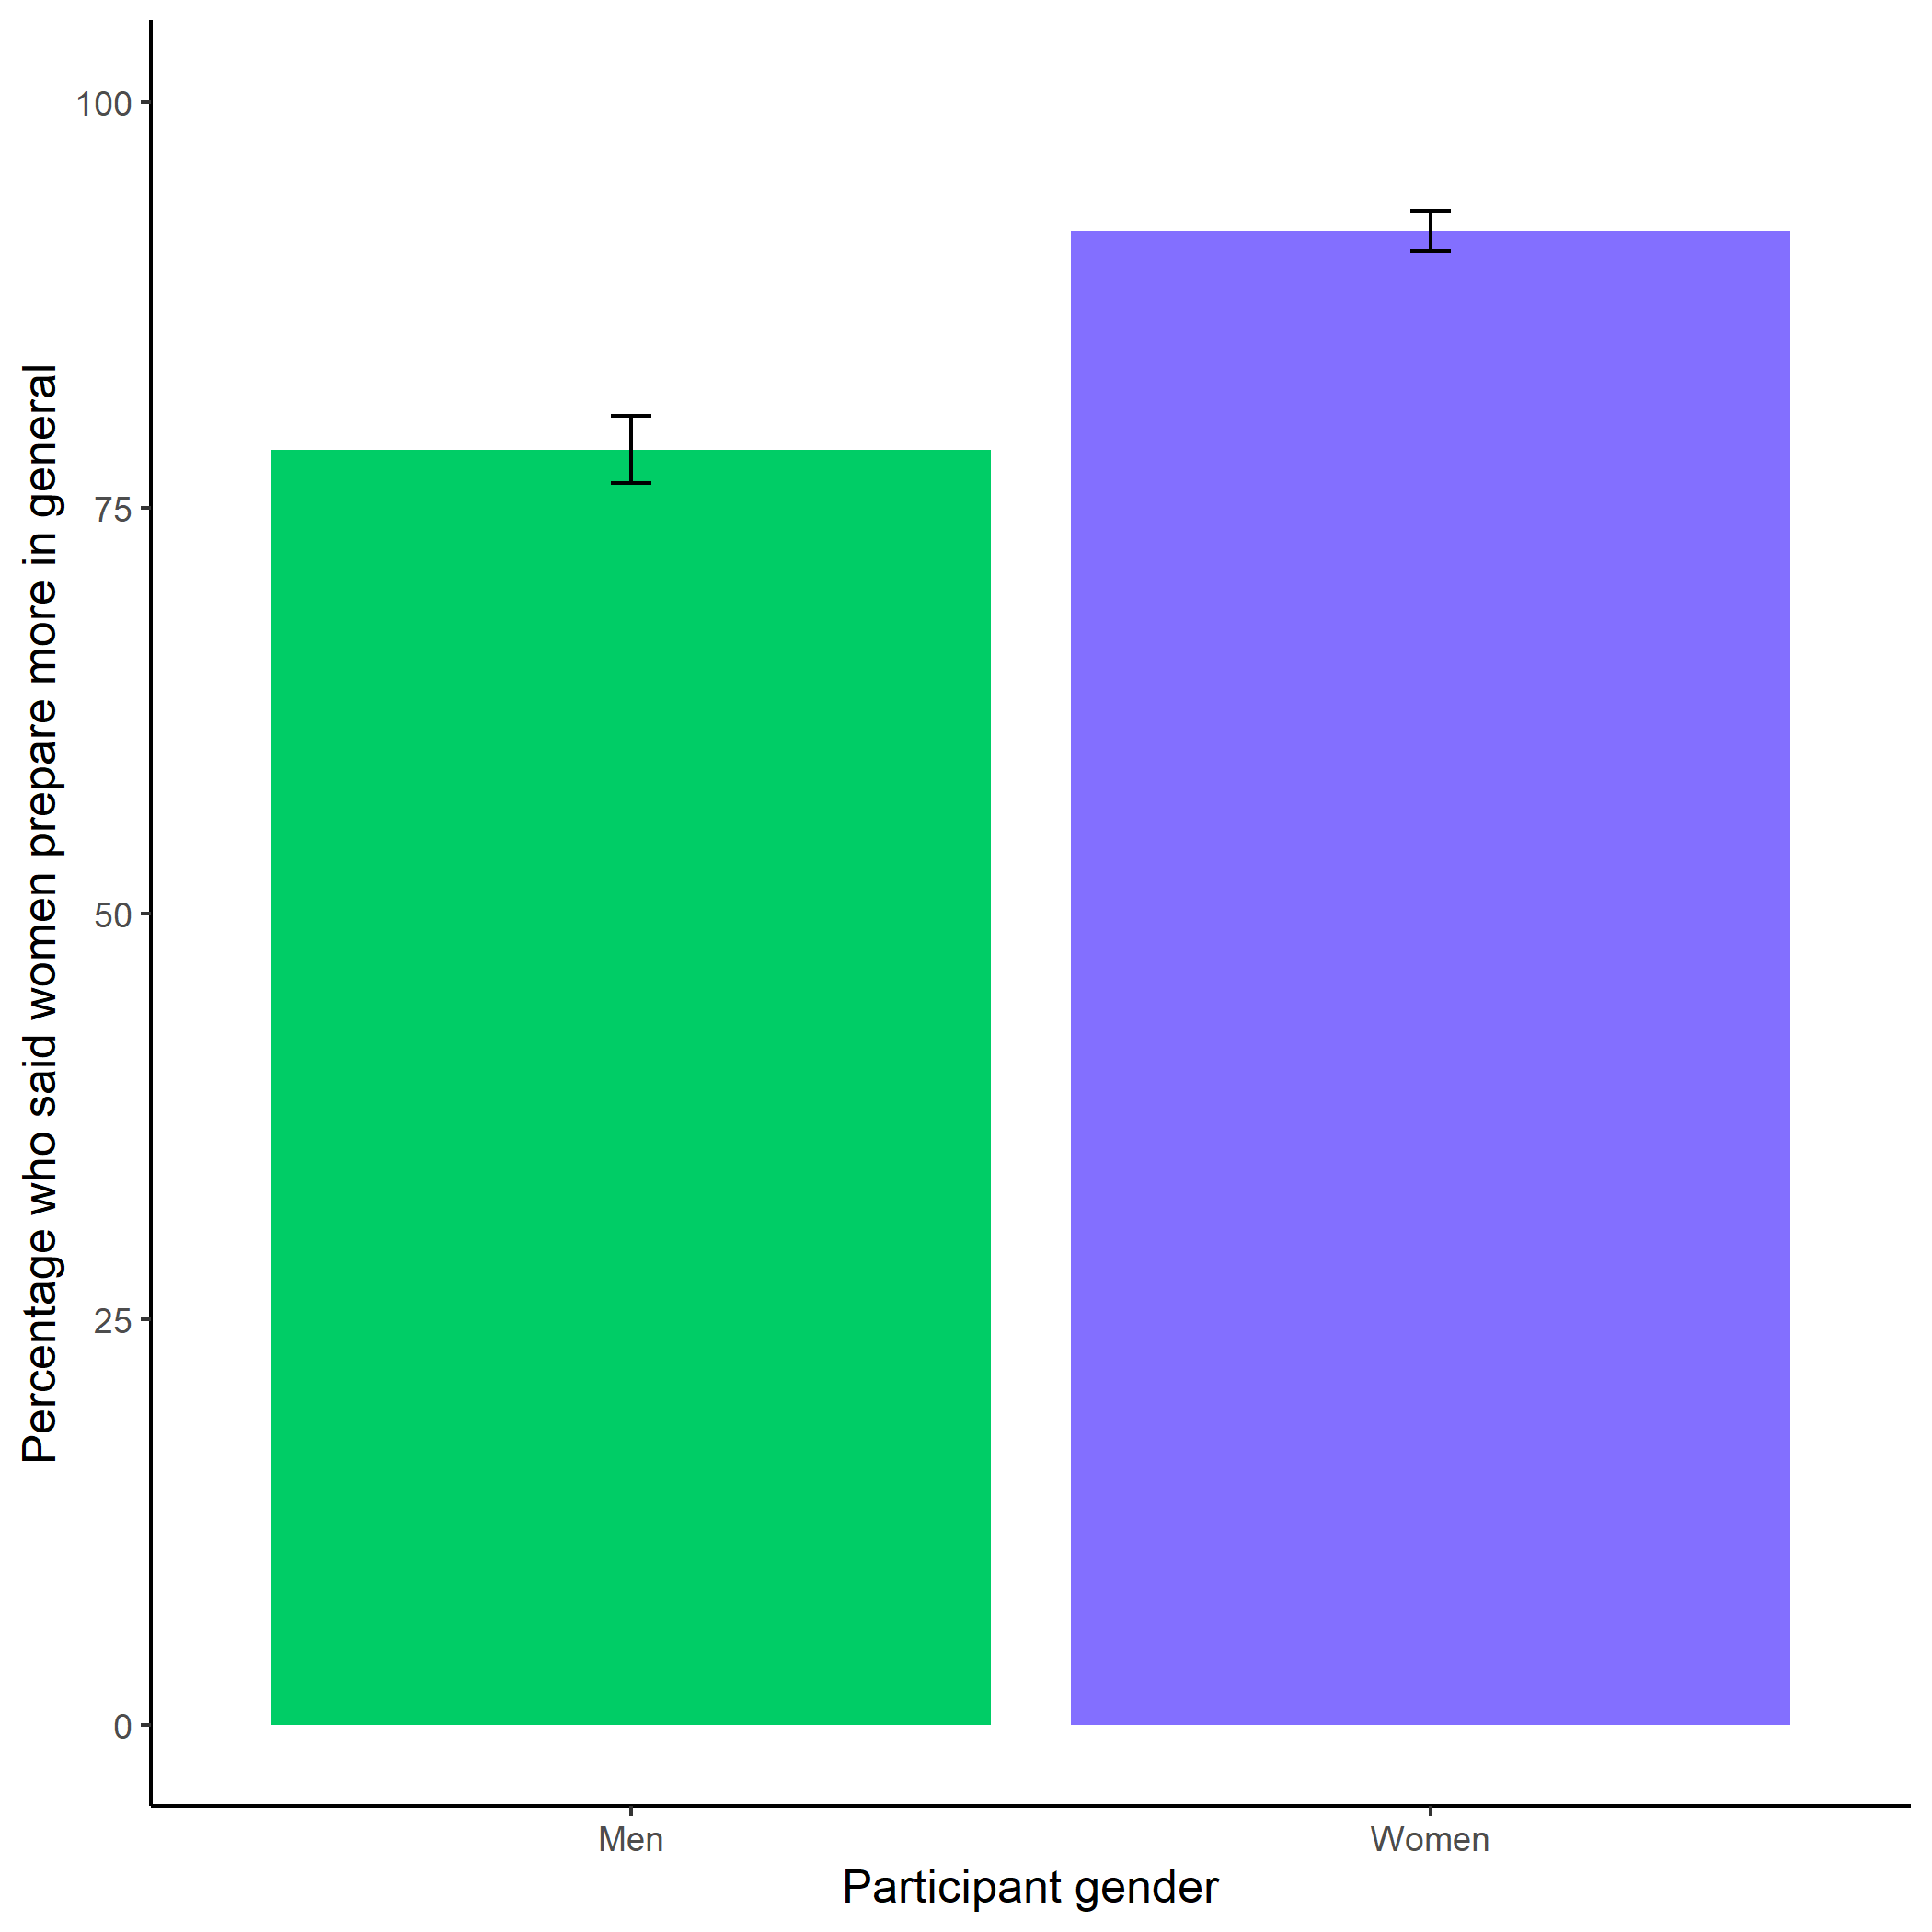
\includegraphics[width=29.17in]{C:/Users/keana/OneDrive - PennO365/Comp_transfer2018/Penn/practice_study/gender-practice/study2/figs/fig03_perc-gen-gender-pract} \caption{Participants' perceptions of general gender differences in choice to prepare. We replicate the findings from Study 1, where participants (especially women) are significantly more likely than chance to state that women prepare more in general than men. Error bars represent standard errors.}\label{fig:s203}
\end{figure}

\begin{figure}
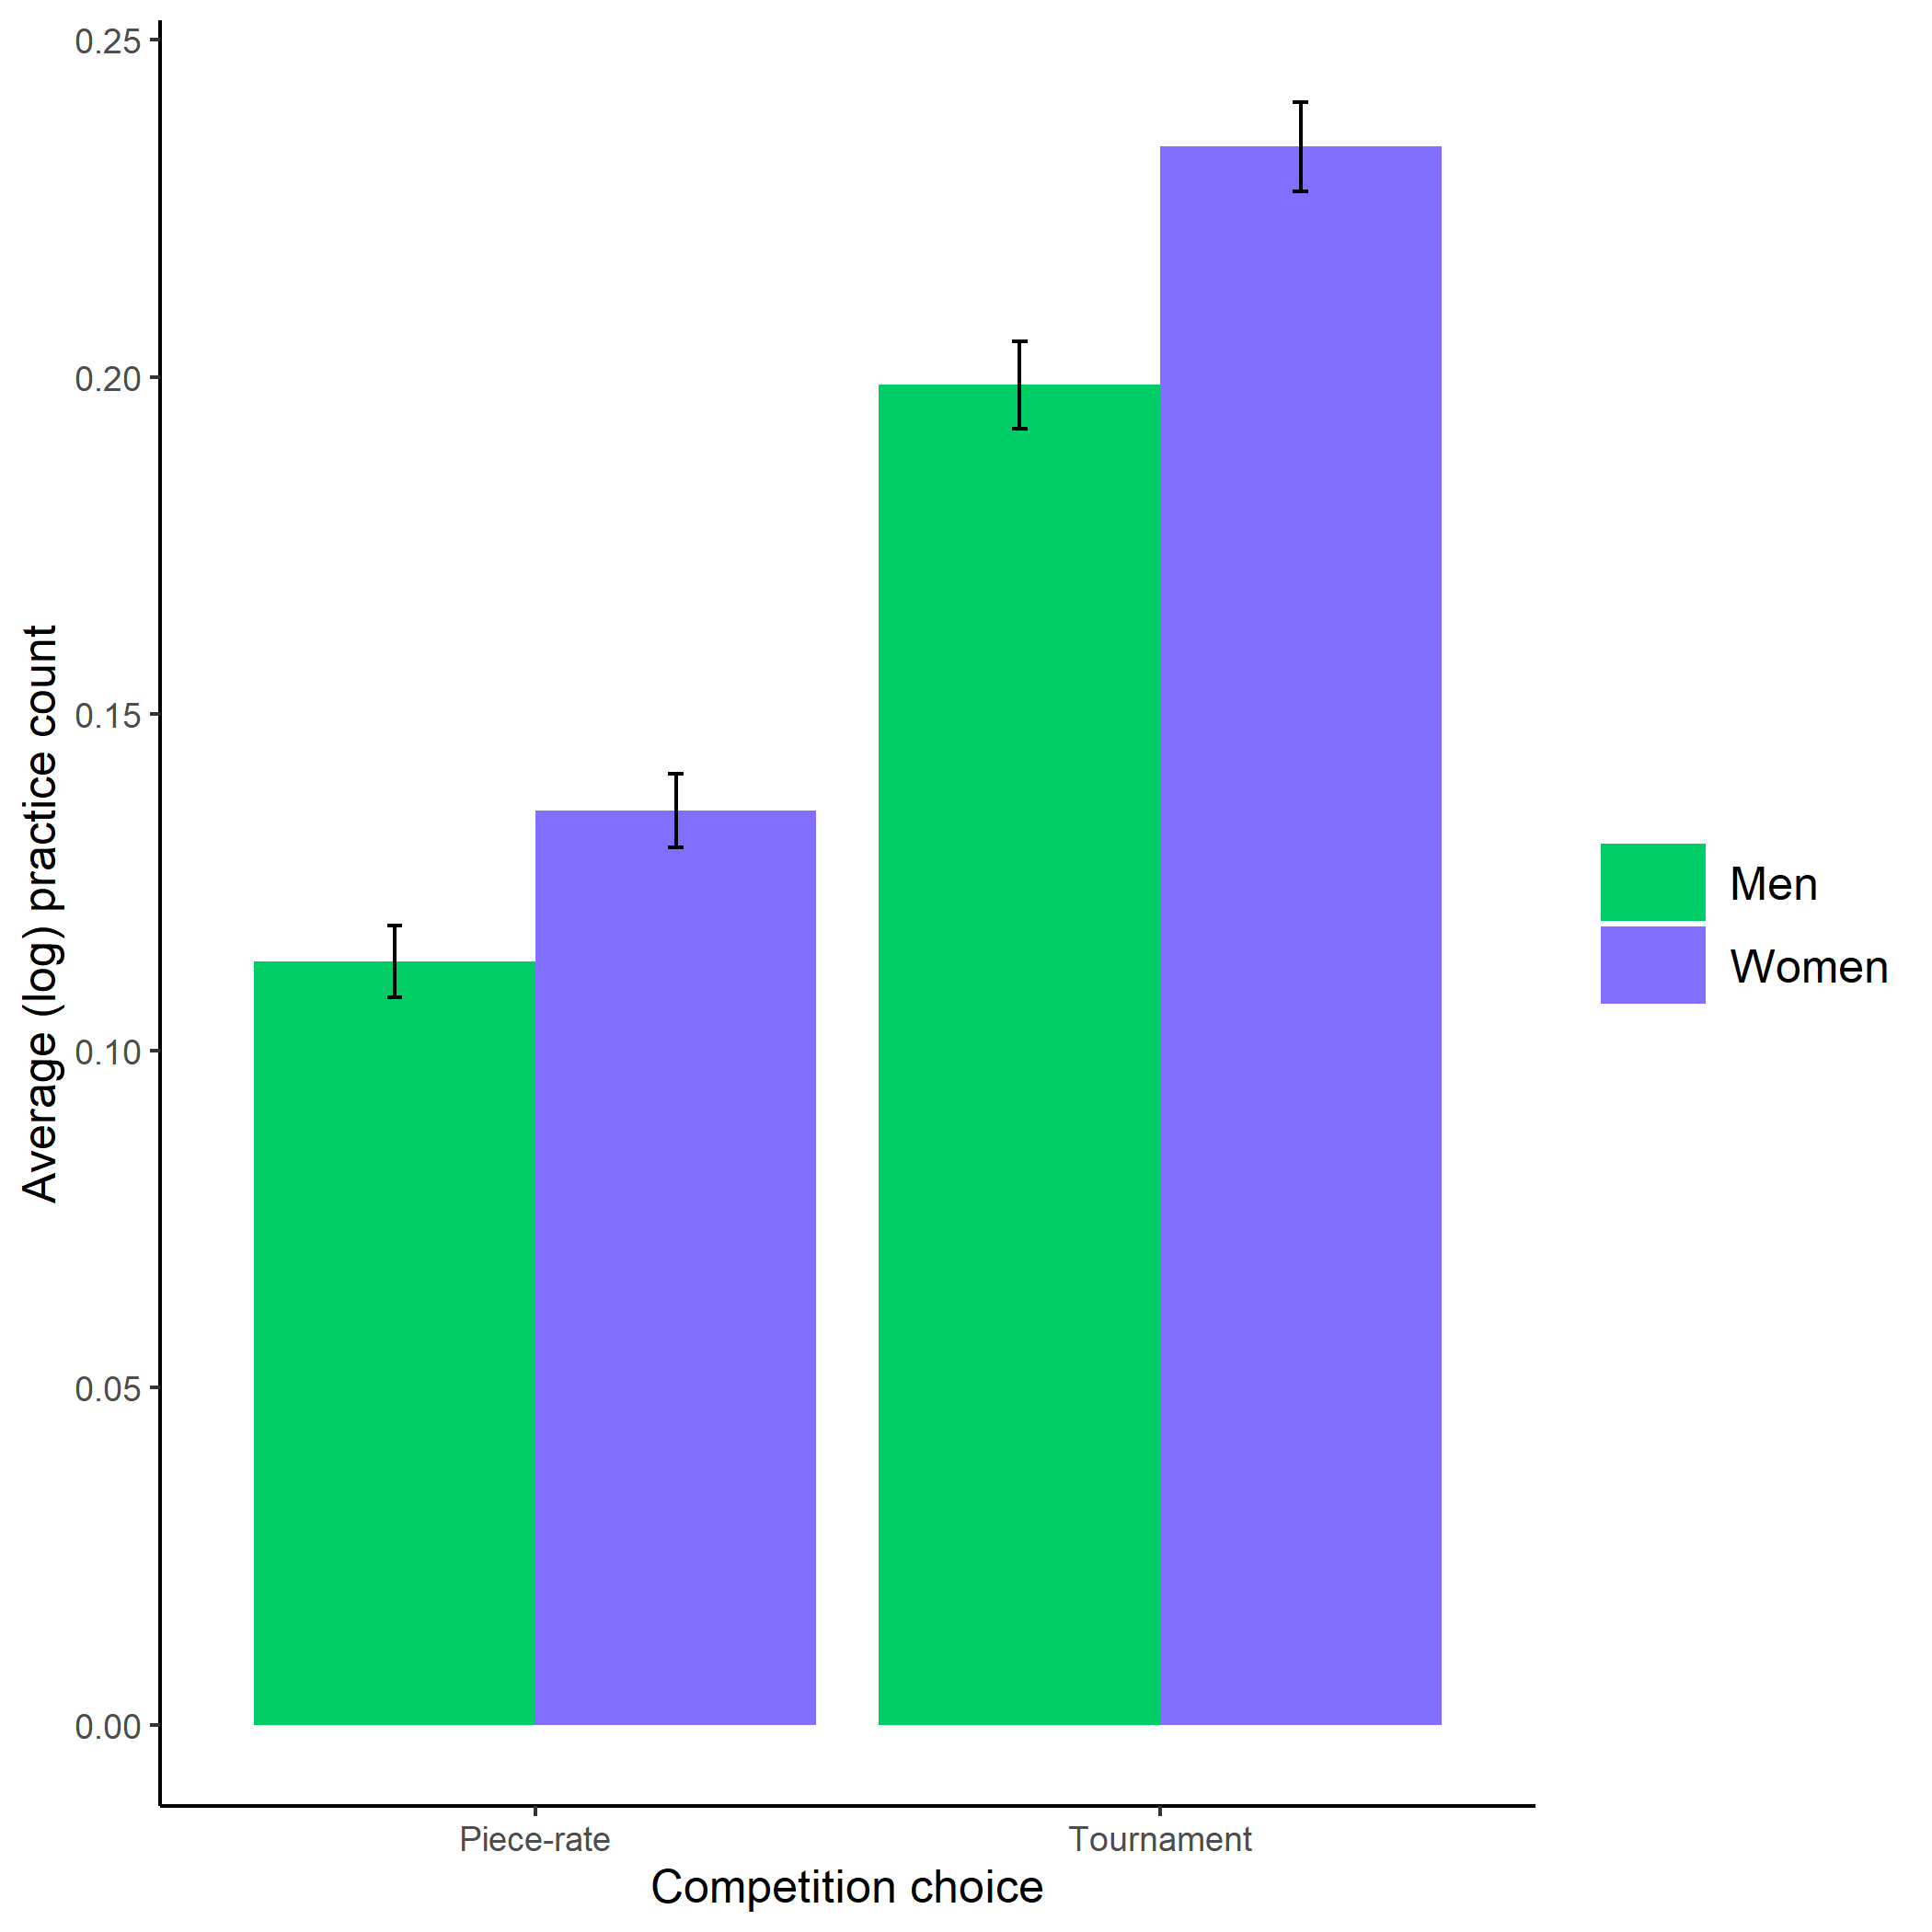
\includegraphics[width=29.17in]{C:/Users/keana/OneDrive - PennO365/Comp_transfer2018/Penn/practice_study/gender-practice/study2/figs/fig04_total-rev-count-by-gender-comp-choice} \caption{Gender differences in the number of extra preparation rounds chosen across participants' choice in a payment scheme. Here, we show that the gender gap in the choice to prepare is robust, even when half of the women are forced to prepare in the preparation condition. Error bars represent standard errors.}\label{fig:s204}
\end{figure}

\hypertarget{study-3-1}{%
\section{Study 3}\label{study-3-1}}

\begin{figure}
\includegraphics[width=29.17in]{C:/Users/keana/OneDrive - PennO365/Comp_transfer2018/Penn/practice_study/gender-practice/study4/figs/fig00_comp-choice-women-by-cond} \caption{Proportion of participants that identify as women who chose to compete by condition. We do not find evidence of the hypothesized effect of condition on the choice to compete. On the contrary, women in the control condition were significantly more likely to choose to compete than women in the preparation condition. Error bars represent standard errors.}\label{fig:s300}
\end{figure}

\begin{figure}
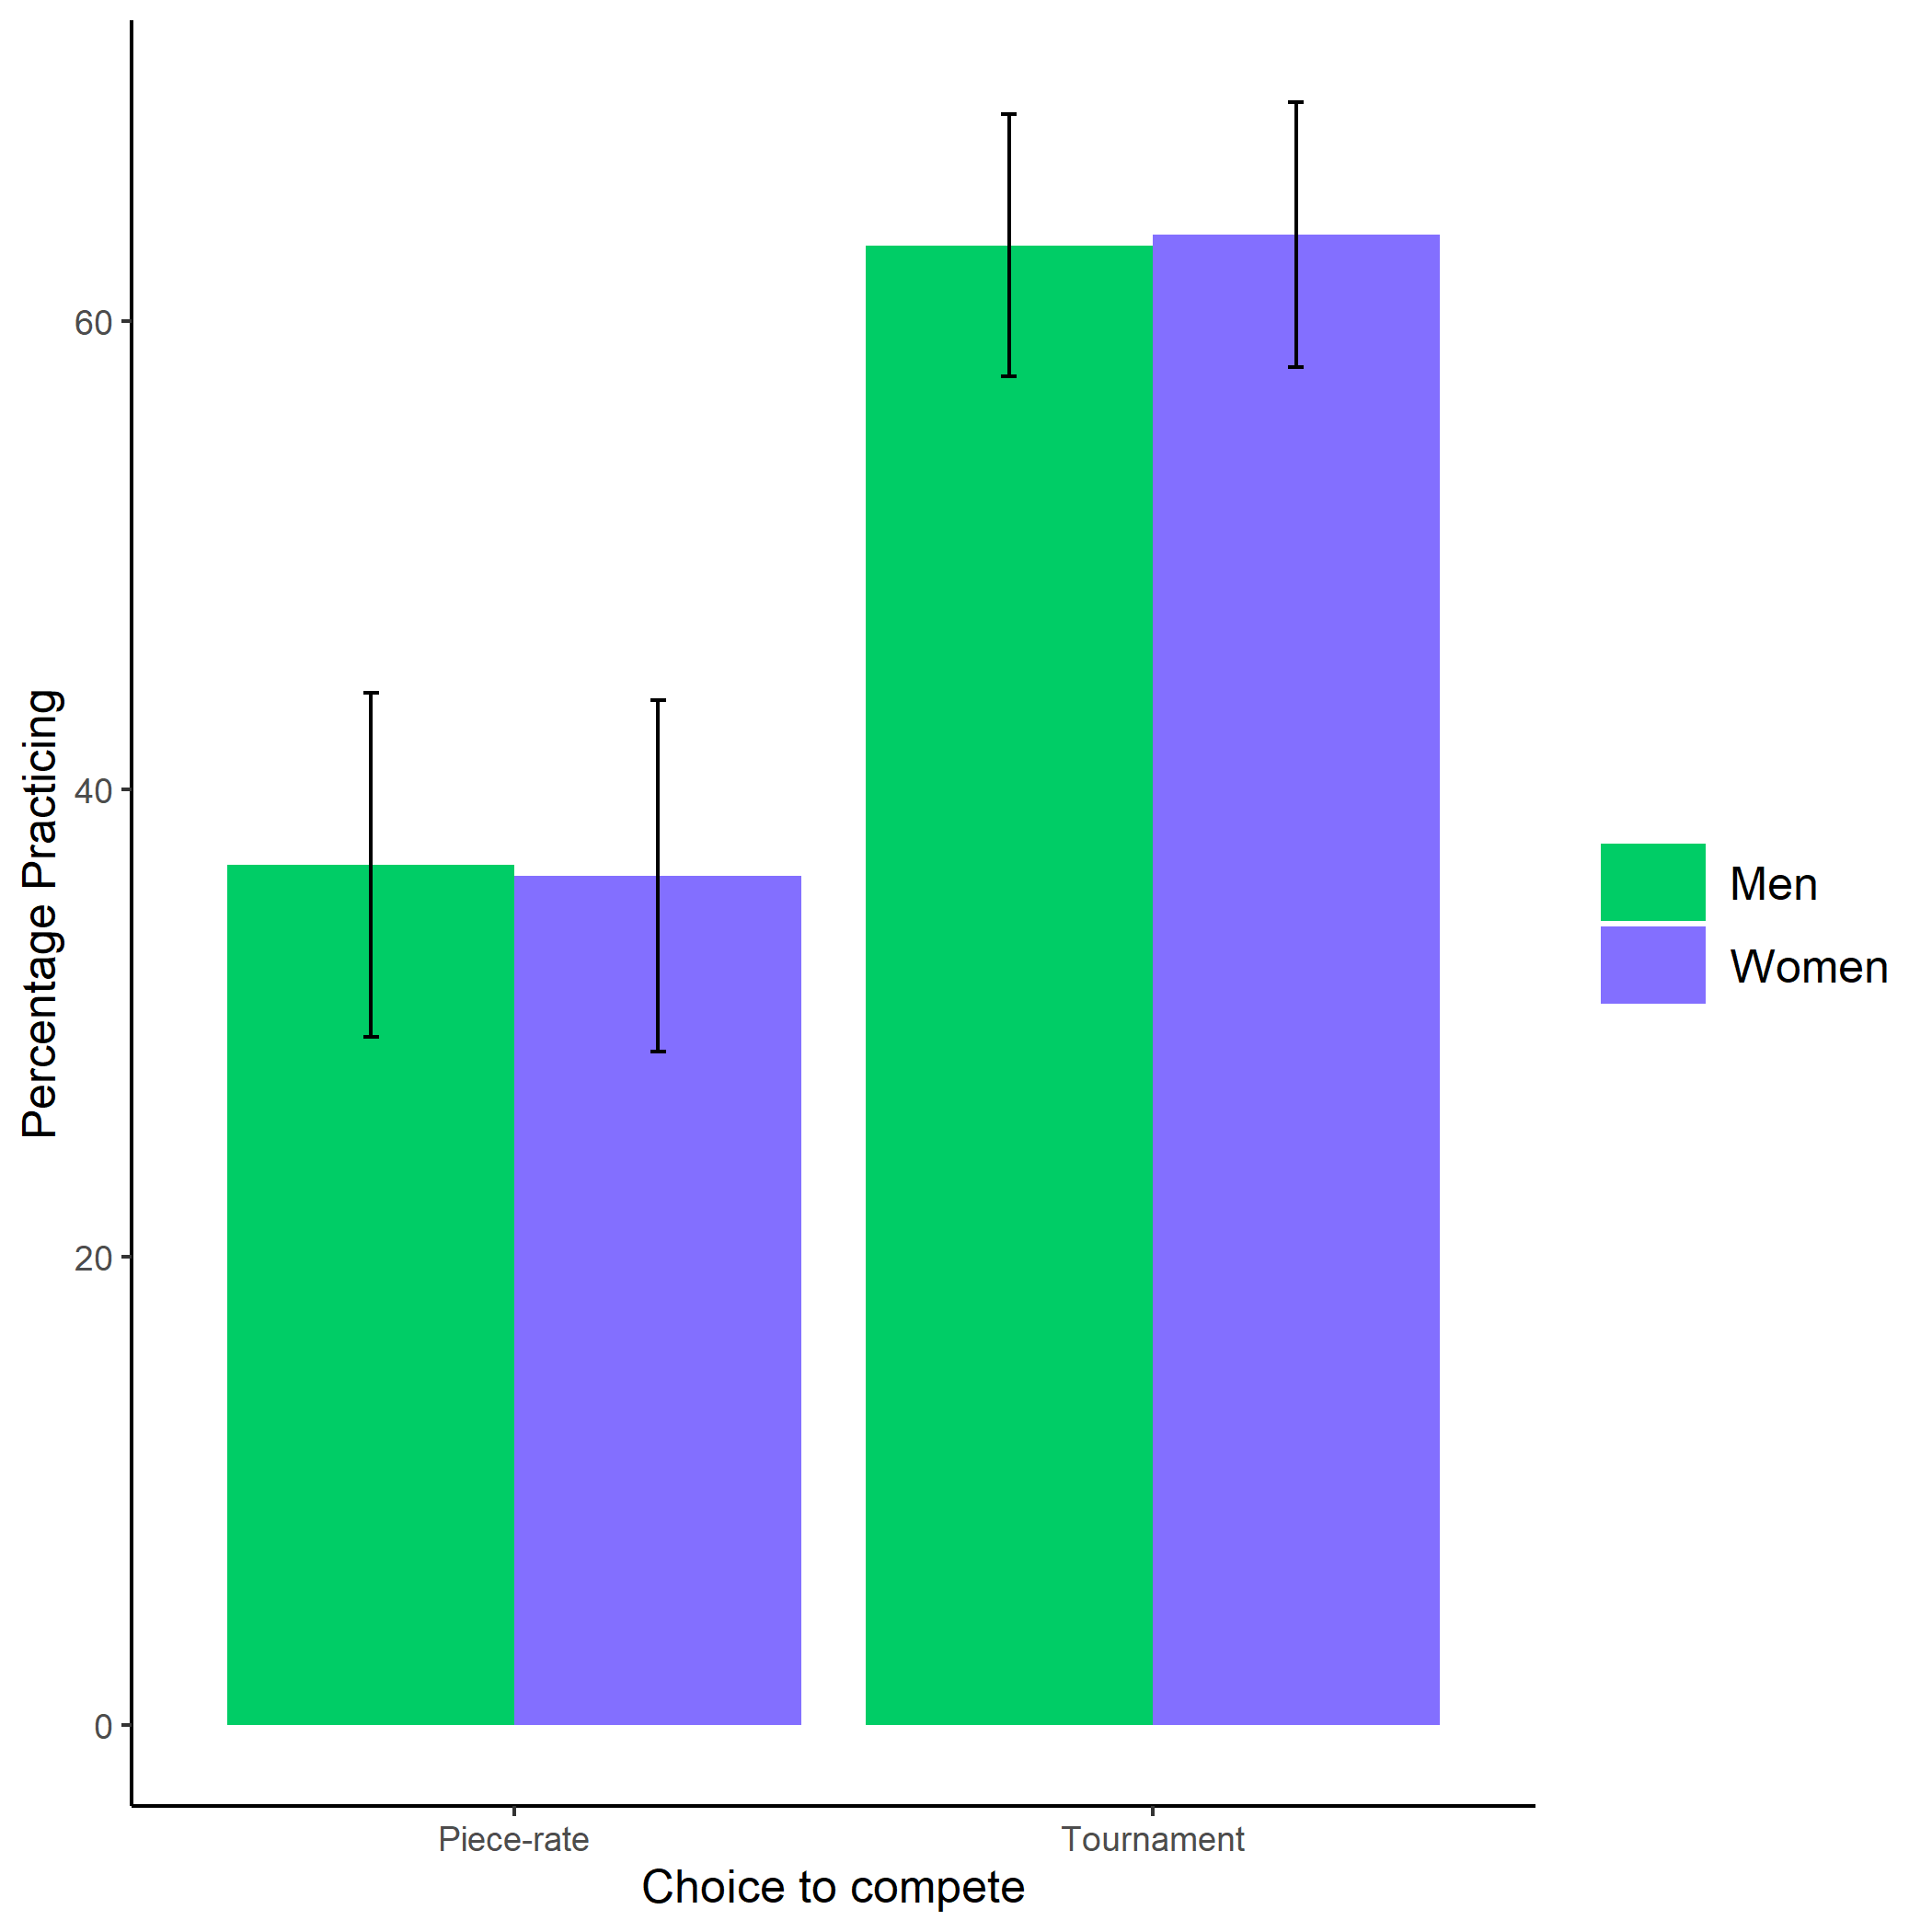
\includegraphics[width=29.17in]{C:/Users/keana/OneDrive - PennO365/Comp_transfer2018/Penn/practice_study/gender-practice/study4/figs/fig01_pract-choice-by-gender-and-cond-bar} \caption{Proportion of participants who chose to compete by condition and gender. Error bars represent standard errors.}\label{fig:s301}
\end{figure}


%%%%% REFERENCES

% JEM: Quote for the top of references (just like a chapter quote if you're using them).  Comment to skip.
% \begin{savequote}[8cm]
% The first kind of intellectual and artistic personality belongs to the hedgehogs, the second to the foxes \dots
%   \qauthor{--- Sir Isaiah Berlin \cite{berlin_hedgehog_2013}}
% \end{savequote}

\setlength{\baselineskip}{0pt} % JEM: Single-space References

{\renewcommand*\MakeUppercase[1]{#1}%
\printbibliography[heading=bibintoc,title={\bibtitle}]}

\end{document}
